\documentclass[twoside,11pt]{article}

% JMLR imports
\usepackage{jmlr2e}
\usepackage{amsmath,amssymb,amsfonts}
\usepackage{booktabs}
\usepackage{multirow}
\usepackage{graphicx}
\usepackage{subcaption}
\usepackage{algorithm}
\usepackage{algorithmic}
\usepackage{xcolor}
\usepackage[hidelinks]{hyperref}

% Custom commands
\newcommand{\R}{\mathbb{R}}
\newcommand{\btheta}{\boldsymbol{\theta}}
\newcommand{\bmu}{\boldsymbol{\mu}}
\newcommand{\bC}{\mathbf{C}}
\newcommand{\bI}{\mathbf{I}}
\newcommand{\calF}{\mathcal{F}}

\newtheorem{conjecture}{Conjecture}

% ========== Blind/Public toggle ==========
% Default: blind. To compile public version:
%   pdflatex "\def\publicmode{}\documentclass[twoside,11pt]{article}

% JMLR imports
\usepackage{jmlr2e}
\usepackage{amsmath,amssymb,amsfonts}
\usepackage{booktabs}
\usepackage{multirow}
\usepackage{graphicx}
\usepackage{subcaption}
\usepackage{algorithm}
\usepackage{algorithmic}
\usepackage{xcolor}
\usepackage[hidelinks]{hyperref}

% Custom commands
\newcommand{\R}{\mathbb{R}}
\newcommand{\btheta}{\boldsymbol{\theta}}
\newcommand{\bmu}{\boldsymbol{\mu}}
\newcommand{\bC}{\mathbf{C}}
\newcommand{\bI}{\mathbf{I}}
\newcommand{\calF}{\mathcal{F}}

\newtheorem{conjecture}{Conjecture}

% ========== Blind/Public toggle ==========
% Default: blind. To compile public version:
%   pdflatex "\def\publicmode{}\documentclass[twoside,11pt]{article}

% JMLR imports
\usepackage{jmlr2e}
\usepackage{amsmath,amssymb,amsfonts}
\usepackage{booktabs}
\usepackage{multirow}
\usepackage{graphicx}
\usepackage{subcaption}
\usepackage{algorithm}
\usepackage{algorithmic}
\usepackage{xcolor}
\usepackage[hidelinks]{hyperref}

% Custom commands
\newcommand{\R}{\mathbb{R}}
\newcommand{\btheta}{\boldsymbol{\theta}}
\newcommand{\bmu}{\boldsymbol{\mu}}
\newcommand{\bC}{\mathbf{C}}
\newcommand{\bI}{\mathbf{I}}
\newcommand{\calF}{\mathcal{F}}

\newtheorem{conjecture}{Conjecture}

% ========== Blind/Public toggle ==========
% Default: blind. To compile public version:
%   pdflatex "\def\publicmode{}\documentclass[twoside,11pt]{article}

% JMLR imports
\usepackage{jmlr2e}
\usepackage{amsmath,amssymb,amsfonts}
\usepackage{booktabs}
\usepackage{multirow}
\usepackage{graphicx}
\usepackage{subcaption}
\usepackage{algorithm}
\usepackage{algorithmic}
\usepackage{xcolor}
\usepackage[hidelinks]{hyperref}

% Custom commands
\newcommand{\R}{\mathbb{R}}
\newcommand{\btheta}{\boldsymbol{\theta}}
\newcommand{\bmu}{\boldsymbol{\mu}}
\newcommand{\bC}{\mathbf{C}}
\newcommand{\bI}{\mathbf{I}}
\newcommand{\calF}{\mathcal{F}}

\newtheorem{conjecture}{Conjecture}

% ========== Blind/Public toggle ==========
% Default: blind. To compile public version:
%   pdflatex "\def\publicmode{}\input{covariance_drift}"
\ifdefined\publicmode
  \newcommand{\blindmode}{0}
\else
  \newcommand{\blindmode}{1}
\fi

% \jmlrheading to be filled by JMLR editorial office
\jmlrheading{}{}{}{}{}{}

\ShortHeadings{Covariance-Induced Irreversible Drift in Constrained Search}{}

\begin{document}

\title{Cross-Dimensional Covariance Adaptation Induces Irreversible Drift\\
Toward Deceptive Attractors in Barrier-Constrained Search}

\ifnum\blindmode=1
  \author{\name Anonymous \\
         \addr Anonymous Institution}
\else
  \author{\name Alex Chengyu Li \\
         \addr Independent Researcher, Tokyo, Japan \\
         \addr \texttt{cl7076@nyu.edu}}
\fi

\editor{}

\maketitle

\begin{abstract}
We report a failure mode of CMA-ES in constrained optimization:
\emph{covariance-induced irreversible drift}. On a barrier-constrained
search problem, full CMA-ES initially discovers feasible,
low-overhead solutions but progressively amplifies redundant parameter
dimensions through cross-dimensional covariance adaptation, trading
constraint feasibility for marginal objective improvement. Once entered,
the resulting deceptive attractor basin resists all tested local
interventions: in extended 3000-generation escape attempts, full CMA-ES
returns to the feasible regime in only 1/10 trials, while sep-CMA-ES
returns in 5/5 and frozen-covariance search in 4/5, confirming that
learned covariance structure maintains the lock. In a 30-seed controlled
comparison, full CMA-ES drifts in
73\% of runs versus 43\% for sep-CMA-ES and 16\% for isotropic ES
(Fisher's exact $p = 0.018$, Mann-Whitney $p = 0.001$).
Controlled ablations on the actual problem confirm that cross-dimensional
interactions (C2) are necessary ($p = 0.0002$ when Spearman is replaced
with MSE), while population scaling experiments show monotonically
non-decreasing drift separation: from 30 percentage points at $\lambda = 17$
to complete separation (100\% vs.\ 0\%) at $\lambda = 200$.
\end{abstract}

\begin{keywords}
  CMA-ES, constrained optimization, deceptive attractors, evolution strategies,
  irreversible drift, constraint handling, black-box optimization
\end{keywords}

%% ============================================================
\section{Introduction}
\label{sec:intro}
%% ============================================================

The Covariance Matrix Adaptation Evolution Strategy (CMA-ES;
\citealt{hansen2001completely,hansen2016cma}) is among the most effective
derivative-free optimizers for continuous black-box problems. CMA-ES
learns a full covariance matrix $\bC$ that captures pairwise parameter
dependencies, enabling the search distribution to align with the local
objective landscape. This cross-dimensional adaptation is the standard explanation for
CMA-ES's superiority over simpler evolution strategies on non-separable
problems~\citep{hansen2003reducing,ros2008simple}.

Standard constraint-handling approaches (penalty functions~\citep{smith1997penalty},
feasibility rules~\citep{deb2000efficient}, and augmented Lagrangian
methods~\citep{atamna2016augmented}) manage the interaction between objective
improvement and constraint satisfaction. \citet{arnold2012cmaes} study how
CMA-ES adapts near constraint boundaries, and
\citet{kramer2010cmaes} review boundary-handling mechanisms. Despite this
work, the interaction between CMA-ES's covariance adaptation and constraint
structure has not been characterized for binary (pass/fail) constraints,
which arise in safety-constrained policy search~\citep{garciarl2015safe},
fairness-constrained classification~\citep{agarwal2018fairness}, and algorithm
configuration~\citep{hutter2011smac}.

We report a setting where cross-dimensional covariance adaptation becomes
pathological. In barrier-constrained search, where candidate solutions must
satisfy binary feasibility constraints while optimizing a non-smooth
objective, full covariance adaptation systematically discovers and amplifies
parameter dimensions that provide marginal objective improvement at the cost
of constraint compliance. The resulting \emph{covariance-induced irreversible
drift} cannot be reversed by any tested local search intervention. This
pathology is absent in restricted covariance variants (diagonal and isotropic),
establishing it as a consequence of cross-dimensional adaptation interacting
with the constraint structure, not an inherent property of the fitness
landscape.

Our experimental domain is the search for complexity measures of Boolean
functions that predict circuit size while respecting three complexity-theoretic
barrier constraints~\citep{razborov1997natural,baker1975relativizations,aaronson2008algebrization}.
This domain combines three structural properties:
(i)~a non-smooth, rank-based objective;
(ii)~high-dimensional quadratic parameter interactions; and
(iii)~discontinuous constraint boundaries.
While our findings are established on this specific domain, the structural
conditions are not unique to it, and we conjecture the phenomenon may arise in
other constrained optimization settings sharing these properties.

\subsection{Contributions}

\begin{enumerate}
\item \textbf{Phenomenon characterization.} We document covariance-induced
  irreversible drift, in which full CMA-ES systematically transitions from
  feasible solutions to infeasible ones through cross-dimensional covariance
  adaptation, and trace the complete causal pathway (Section~\ref{sec:drift},
  \ref{sec:mechanism}).

\item \textbf{Multi-basin compliance landscape.} We characterize the
  barrier-constrained fitness landscape as containing three qualitatively
  distinct solution types separated by deep infeasible valleys
  (Section~\ref{sec:landscape}).

\item \textbf{Cross-optimizer dissection (30 seeds).} We establish that drift
  is specific to full covariance adaptation through a 30-seed controlled
  comparison: full CMA-ES drifts in 73\% of runs, sep-CMA-ES in 43\%,
  and isotropic ES in 16\% (Fisher $p = 0.018$; Section~\ref{sec:crossopt}).

\item \textbf{Controlled ablation of structural conditions.} We test the
  irreducibility conjecture by same-problem ablation: replacing Spearman with
  MSE (C1) reduces but does not eliminate the full$>$sep differential
  ($p = 0.0002$); replacing binary with soft penalties (C3) narrows the gap
  (66\% vs.\ 40\%, $p = 0.035$). Cross-dimensional adaptation (C2) is the
  primary driver (Section~\ref{sec:irreducibility}).

\item \textbf{Population scaling law.} Drift separation between full and
  sep-CMA-ES is monotonically non-decreasing in population size $\lambda$, reaching
  complete separation (100\% vs.\ 0\%) at $\lambda = 200$
  (Section~\ref{sec:lambda}).

\item \textbf{Irreversibility characterization.} Extended 3000-generation
  escape attempts confirm asymmetric irreversibility: full CMA-ES returns
  to Type~C in 1/10 trials, while sep-CMA-ES returns in 5/5 and
  frozen-covariance in 4/5 (Section~\ref{sec:irreversibility}).
\end{enumerate}

%% ============================================================
\section{Related Work}
\label{sec:related}
%% ============================================================

\textbf{CMA-ES theory and variants.}
CMA-ES~\citep{hansen2001completely} learns the full covariance structure of
beneficial perturbations through rank-one and rank-$\mu$ updates. The
sep-CMA-ES variant~\citep{ros2008simple} restricts adaptation to diagonal
entries, achieving linear time complexity at the cost of cross-dimensional
learning. Restart strategies~\citep{auger2005restart} address premature
convergence by resetting the search distribution. Our work identifies a
setting where restarts catalyze drift rather than prevent stagnation.

\textbf{Constrained CMA-ES.}
Several approaches to constraint handling in CMA-ES have been proposed.
\citet{arnold2012cmaes} analyze adaptation near linear constraint
boundaries for (1+1)-CMA-ES. \citet{kramer2010cmaes} review boundary-handling
mechanisms including resampling and projection. \citet{atamna2016augmented}
combine CMA-ES with augmented Lagrangian methods for continuous constraints.
These works address continuous constraints with smooth boundaries.
Our setting has binary (pass/fail) constraints and a non-smooth (rank-based)
objective. The interaction of covariance adaptation with discontinuous
constraint boundaries creates a pathology distinct from the step-size
difficulties documented for smooth constraints.

\textbf{Deceptive fitness landscapes.}
Deception in evolutionary computation, where selection pressure drives the
population away from the global optimum, has been studied since
\citet{goldberg1987simple} and formalized by \citet{whitley1991fundamental}.
Here, however, the deception is \emph{optimizer-specific}:
the same landscape is non-deceptive for sep-CMA-ES and isotropic ES but
deceptive for full CMA-ES. The deception arises from the interaction between
the optimizer's covariance adaptation and the constraint structure, not from
the fitness function alone.

\textbf{Non-smooth optimization.}
CMA-ES is commonly applied to noisy and non-smooth
objectives~\citep{hansen2009benchmarking}. On rank-based or ordinal objectives,
the covariance matrix estimates the local ranking structure rather than the
Hessian. Our results show that this rank-based learning mechanism can discover
spurious cross-dimensional couplings that exploit constraint boundary
geometry.

\textbf{Algorithm selection and configuration.}
The finding that optimizer variant choice (full vs.\ sep-CMA-ES) determines
feasibility is an instance of the algorithm selection
problem~\citep{rice1976algorithm,xu2008satzilla}. In the algorithm
configuration framework~\citep{hutter2011smac,lindauer2022smac3}, our result
implies that covariance structure should be treated as a configurable
hyperparameter whose optimal setting depends on constraint type.

\textbf{Complexity-theoretic barriers.}
The natural proofs barrier~\citep{razborov1997natural}, relativization
barrier~\citep{baker1975relativizations}, and algebrization
barrier~\citep{aaronson2008algebrization} are foundational results in
computational complexity theory. Our use of these barriers as optimization
constraints is new.

%% ============================================================
\section{Problem Setup}
\label{sec:setup}
%% ============================================================

\subsection{Boolean Function Complexity Measures}

Let $\calF_n = \{f : \{0,1\}^n \to \{0,1\}\}$ denote the set of Boolean functions
on $n$ variables. For each $f \in \calF_n$, we compute a vector of $D=10$
structural features $\mathbf{m}(f) \in \R^D$ (Table~\ref{tab:features}).

\begin{table}[t]
\caption{Boolean function features used as input dimensions. Each feature
maps a Boolean function $f : \{0,1\}^n \to \{0,1\}$ to $\R$. Definitions
follow standard references~\citep{boppana1990complexity,jukna2012boolean}.
Features are listed alphabetically.
The internal genome uses the storage order given in the code repository
(sensitivity is at storage index~8); all index references in the paper use
the alphabetical convention for readability, with sensitivity at
position~7.}
\label{tab:features}
\centering
\small
\begin{tabular}{lp{8cm}}
\toprule
Feature & Description \\
\midrule
Algebraic degree & Degree of the unique multilinear polynomial over GF(2) \\
Autocorrelation sum & $\sum_{s \neq 0} |\Delta_f(s)|$ where $\Delta_f(s) = \sum_x (-1)^{f(x) \oplus f(x \oplus s)}$ \\
Gzip ratio & Compression ratio of the truth table under gzip \\
Influence (total) & Sum of individual variable influences $\sum_i \Pr[f(x) \neq f(x^{\oplus i})]$ \\
LZ76 complexity & Lempel-Ziv compression complexity of the truth table \\
Nonlinearity & Hamming distance to the nearest affine function \\
Run length & Longest run of consecutive identical bits in the truth table \\
Sensitivity & Average sensitivity: mean over inputs $x$ of the number of bit positions $i$ with $f(x) \neq f(x^{\oplus i})$ \\
Shannon entropy & Entropy of the truth table viewed as a binary string \\
Spectral entropy & Shannon entropy of the squared Fourier spectrum \\
\bottomrule
\end{tabular}
\end{table}

A \emph{parameterized complexity measure} $\mu_\btheta : \calF_n \to \R$ is defined as:
\begin{equation}
\label{eq:measure}
\mu_\btheta(f) = \mathbf{w}^\top \mathbf{m}(f)
  + \mathbf{q}^\top \operatorname{vech}\bigl(\mathbf{m}(f)\,\mathbf{m}(f)^\top\bigr)
  + \mathbf{a}^\top \operatorname{relu}\bigl(\mathbf{m}(f) - \mathbf{t}\bigr),
\end{equation}
where $\operatorname{vech}(\cdot)$ extracts the $D(D+1)/2$ unique entries of the
symmetric outer product (i.e., $\{m_i(f) \cdot m_j(f) : 1 \leq i \leq j \leq D\}$), and $\btheta = (\mathbf{w}, \mathbf{q}, \mathbf{a}, \mathbf{t})$
comprises $D$ linear weights, $D(D+1)/2 = 55$ quadratic weights, $D$ activation
coefficients, and $D$ threshold parameters, totaling $p = 85$ dimensions.

\subsection{Dataset and Objective}

We use $N = 616{,}126$ equivalence classes of Boolean functions on $n=5$
variables under input negation, input permutation, and output negation
(NPN equivalence),
enumerated by \citet{knuth2011art} with exact minimum circuit sizes.
The full space $|\calF_5| = 2^{2^5} = 2^{32} \approx 4.3 \times 10^9$ is
reduced to 616K representatives; each class shares a common minimum circuit size.

The search objective is the Spearman rank correlation:
\begin{equation}
\label{eq:objective}
\rho(\btheta) = \operatorname{Spearman}\bigl(\{\mu_\btheta(f_i)\}_{i=1}^N,\;
  \{s(f_i)\}_{i=1}^N\bigr).
\end{equation}
Spearman correlation is a piecewise-constant function of the continuous
parameters $\btheta$: perturbations that do not change the rank ordering of
$\mu_\btheta(f_i)$ values have zero effect, while perturbations at rank-swap
boundaries produce discontinuous changes. In 85 dimensions with $N \approx 616$K
functions, the function is locally constant almost everywhere, with
discontinuous jumps at rank-swap boundaries.

The effective fitness function incorporates L2 regularization:
$F(\btheta) = \rho(\btheta) - \alpha_{\text{reg}} \|\btheta\|_2^2$, where
$\alpha_{\text{reg}} = 10^{-3}$.

\subsection{Barrier Constraints}

Three constraints define hard feasibility. A genome $\btheta$ is \emph{feasible}
if and only if it passes all three simultaneously:

\begin{enumerate}
\item \textbf{Natural proofs (NP)}~\citep{razborov1997natural}: we sample 10{,}000
  uniformly random Boolean functions $g : \{0,1\}^n \to \{0,1\}$ (not in the
  dataset), compute $\mu_\btheta(g)$ for each, and measure the fraction with
  $|\mu_\btheta(g)| \geq \operatorname{median}(\{|\mu_\btheta(f_i)|\}_{i=1}^N)$,
  where the median is computed over the \emph{dataset} functions. This fraction
  must not exceed $\tau_{\text{NP}} = 1/n^2 = 0.04$.
  Intuitively, a ``useful'' measure (in the Razborov-Rudich sense) assigns large
  values to random functions as readily as to structured ones; a non-natural measure
  assigns large values primarily to structured functions, so random functions
  rarely exceed the dataset median.

\item \textbf{Relativization}~\citep{baker1975relativizations}: the $R^2$ of a
  degree-2 polynomial fit from the $2^n$-dimensional truth-table vector to
  $\mu_\btheta(f)$ must fall below $\tau_{\text{rel}} = 0.99$. This is a proxy for
  oracle independence: a measure that can be accurately predicted from truth-table
  bits alone does not escape relativization.

\item \textbf{Algebrization}~\citep{aaronson2008algebrization}: the fraction of
  $|\mu_\btheta|$-mass on features that admit algebraic extension
  (Shannon entropy, spectral entropy, algebraic degree, nonlinearity,
  autocorrelation sum---features defined via polynomial or Fourier structure
  over the Boolean hypercube) must fall below $\tau_{\text{alg}} = 0.8$.
  The remaining features (LZ76, run length, gzip ratio, sensitivity,
  influence) are classified as non-extensible because they depend on the
  lexicographic or input-enumeration ordering of the truth table, which has
  no natural algebraic extension.
\end{enumerate}

These constraints are binary (pass/fail) and interact non-trivially: the
relativization and algebrization barriers are individually non-binding in our
experiments, but the natural proof barrier actively constrains the feasible
region. The intersection of all three creates the multi-basin landscape
described in Section~\ref{sec:landscape}.

\textbf{Limitation.} These barrier implementations are heuristic proxies inspired
by the complexity-theoretic conditions, not exact implementations thereof.
Our findings characterize optimizer behavior on these specific constraint
implementations. The qualitative landscape structure (multi-basin, disconnected)
is expected to be robust to threshold choices, but the specific basin locations
and volumes depend on the proxy definitions.

\subsection{Optimizer Variants}

We compare three CMA-ES variants differing only in covariance structure:

\begin{itemize}
\item \textbf{Full CMA-ES}: adapts the complete $p \times p$ covariance matrix
  $\bC$, learning all pairwise parameter dependencies.
\item \textbf{sep-CMA-ES}~\citep{ros2008simple}: restricts $\bC$ to a diagonal
  matrix, adapting per-dimension step sizes without cross-dimensional correlations.
\item \textbf{Isotropic ES}: uses the CMA-ES mean update rule but freezes
  $\bC = \bI$ throughout, adapting only the global step size $\sigma$ via
  cumulative step-size adaptation (CSA). No rank-one or rank-$\mu$ covariance
  updates are performed.
\end{itemize}

All variants share population size $\lambda = 100$ (larger than the default
$\lambda \approx 17$ for $p = 85$ to improve feasibility sampling under binary
constraints), initial step size $\sigma_0 = 0.3$, $\sigma_{\max} = 100$, and
$\sigma_{\min} = 10^{-6}$. Automatic restarts trigger when $\sigma$ falls below
$\sigma_{\min}$.

\subsection{Search Procedure}

\begin{algorithm}[t]
\caption{Barrier-constrained CMA-ES search}
\label{alg:search}
\begin{algorithmic}[1]
\STATE Initialize $\btheta_{\text{mean}} \sim \mathcal{N}(0, \bI)$, $\sigma = \sigma_0$, $\bC = \bI$
\FOR{generation $g = 1$ to $G_{\max}$}
  \STATE Sample $\lambda$ candidates: $\btheta_k = \btheta_{\text{mean}} + \sigma \cdot \bC^{1/2} \mathbf{z}_k$, $\mathbf{z}_k \sim \mathcal{N}(0, \bI)$
  \STATE Evaluate $F(\btheta_k) = \rho(\btheta_k) - \alpha_{\text{reg}}\|\btheta_k\|_2^2$ for all $k$
  \STATE Check barriers: $\text{feas}_k = \text{NP}(\btheta_k) \wedge \text{Rel}(\btheta_k) \wedge \text{Alg}(\btheta_k)$
  \STATE Rank candidates: feasible first (by $F$), then infeasible (by $F$)
  \STATE Update $\btheta_{\text{mean}}$, $\sigma$, $\bC$ via CMA-ES rules
  \IF{$\sigma < \sigma_{\min}$}
    \STATE Restart: $\sigma \gets \sigma_0$, $\bC \gets \bI$; alternate random/best-ever mean
  \ENDIF
\ENDFOR
\end{algorithmic}
\end{algorithm}

The search procedure (Algorithm~\ref{alg:search}) uses Deb's feasibility
rules~\citep{deb2000efficient}: feasible solutions always rank above infeasible
ones, regardless of fitness value. Feature evaluation is GPU-batched on an
RTX 3090, computing all 10 features for 100 candidates $\times$ 616K functions
in $\sim$50ms per generation. Each 8000-generation run requires approximately
3.5 hours on an RTX 3090 (7 hours with per-generation diagnostics enabled).

%% ============================================================
\section{The Compliance Landscape}
\label{sec:landscape}
%% ============================================================

\subsection{Three Solution Types}

Extended CMA-ES runs (8000 generations, 5 random seeds: 42, 137, 256, 512, 1024)
reveal three qualitatively distinct solution types, classified by the total
sensitivity weight $\phi_{\text{sens}}$ (fraction of genome weight attributable to
sensitivity-related parameters). We additionally report the cross-term fraction
$\phi_{\text{cross}} = \bigl(\sum_{i < 7} |q_{i,7}| + \sum_{j > 7} |q_{7,j}|\bigr) / \sum_{i \leq j} |q_{i,j}|$
(where index 7 denotes the sensitivity feature under alphabetical ordering) as a secondary descriptor of
compliance architecture.

\begin{table}[t]
\caption{Solution type classification across five seeds (8000 generations,
full CMA-ES). $\phi_{\text{sens}}$: fraction of genome magnitude weight
$\sum |w_i| + \sum |q_{i,j}| + \sum |a_i|$ (threshold parameters excluded as
they control gating position, not signal magnitude) attributable to
sensitivity-related parameters. $\phi_{\text{cross}}$: quadratic mass in sensitivity$\times$signal
interactions. The empirical threshold $\phi_{\text{sens}} = 0.05$ separates
Types B and C; we note this is a post-hoc choice (see text).}
\label{tab:types}
\centering
\begin{tabular}{llcccll}
\toprule
Type & Seeds & $\phi_{\text{sens}}$ & $\phi_{\text{cross}}$ & $\rho$ & Feasible & Strategy \\
\midrule
A & 42 & 0.698 & 0.809 & 0.5942 & Yes (0.0186) & Dedicated compliance \\
B & 137 & 0.188 & 0.145 & 0.5967 & No (0.0402) & Embedded compliance \\
B & 256 & 0.239 & 0.151 & 0.5946 & No (0.0402) & Embedded compliance \\
B & 1024 & 0.224 & 0.131 & 0.5956 & Yes (0.0400) & Embedded compliance \\
C & 512 & 0.004 & 0.009 & \textbf{0.5975} & \textbf{Yes} (0.0377) & Pure signal \\
\bottomrule
\end{tabular}
\end{table}

Table~\ref{tab:types} reports per-seed feasibility with natural proof density in
parentheses (threshold: 0.04). Type~B seeds 137 and 256 are infeasible (density
at or marginally above threshold); seed 1024 is exactly at threshold. The
classification boundary at $\phi_{\text{sens}} = 0.05$ is empirically chosen to
separate the observed gap between 0.004 and 0.131; we do not claim this represents
a natural discontinuity without a larger seed sample.

\subsection{Basin Disconnection}

Linear interpolation between all $\binom{5}{2} = 10$ seed pairs
(21 evenly-spaced interpolants per pair, $\btheta_\alpha = (1-\alpha)\btheta_a
+ \alpha\btheta_b$) reveals that solution types occupy largely disconnected
regions in parameter space (Table~\ref{tab:interpolation}).

\begin{table}[t]
\caption{Pairwise linear interpolation between five seed endpoints.
``min $\rho$'' is the worst Spearman correlation along the path; ``max density''
is the peak natural proof density; ``feas.\ pts'' counts interpolants
passing all barriers.}
\label{tab:interpolation}
\centering
\begin{tabular}{llrrr}
\toprule
Path & Types & min $\rho$ & max density & feas.\ pts \\
\midrule
42--256 & A--B & +0.27 & 0.076 & 8/21 \\
137--1024 & B--B & +0.33 & 0.396 & 1/21 \\
42--1024 & A--B & +0.10 & 0.398 & 2/21 \\
42--137 & A--B & $-$0.07 & 0.856 & 1/21 \\
137--512 & B--C & $-$0.16 & 1.000 & 1/21 \\
42--512 & A--C & $-$0.14 & 0.996 & 2/21 \\
\bottomrule
\end{tabular}
\end{table}

We show 6 representative paths (full 10-path table in Appendix~\ref{app:interpolation}).
The interpolation between seeds 42 and 137 (Types~A and~B) is illustrative:
$\rho$ drops to $-0.07$ at $\alpha = 0.2$ (the measure becomes
\emph{anti-correlated} with circuit complexity) while natural proof density peaks
at 0.856. All paths involving seed~512 (Type~C) show extreme disconnection:
max density $\geq 0.958$ and min $\rho$ as low as $-0.16$.

\textbf{Caveat.} Linear interpolation is a lower bound on disconnection.
Two points can share a basin (reachable by a curved feasible path) even if
the linear path between them is entirely infeasible. True connectivity requires
demonstrating the absence of \emph{any} feasible path, which we have not done.
We use ``disconnected'' as shorthand for ``not connected by any tested path.''

\subsection{Basin Robustness}
\label{sec:fragility}

Gaussian perturbation analysis (50 samples per noise level, isotropic) shows
an asymmetry between solution types (Table~\ref{tab:perturbation},
Figure~\ref{fig:perturbation}).

\begin{table}[t]
\caption{Robustness under Gaussian perturbation. 50 samples per noise level.}
\label{tab:perturbation}
\centering
\begin{tabular}{lcccc}
\toprule
$\sigma$ & \multicolumn{2}{c}{Type A (seed 42)} & \multicolumn{2}{c}{Type C (seed 512)} \\
\cmidrule(lr){2-3} \cmidrule(lr){4-5}
 & mean $\rho$ & Feas.\ \% & mean $\rho$ & Feas.\ \% \\
\midrule
0.001 & 0.102 & 34\% & \textbf{0.594} & \textbf{64\%} \\
0.005 & 0.037 & 0\% & 0.520 & 62\% \\
0.010 & 0.023 & 0\% & 0.422 & 56\% \\
0.050 & 0.030 & 0\% & 0.155 & 22\% \\
\bottomrule
\end{tabular}
\end{table}

\begin{figure}[t]
\centering
\begin{subfigure}[t]{\textwidth}
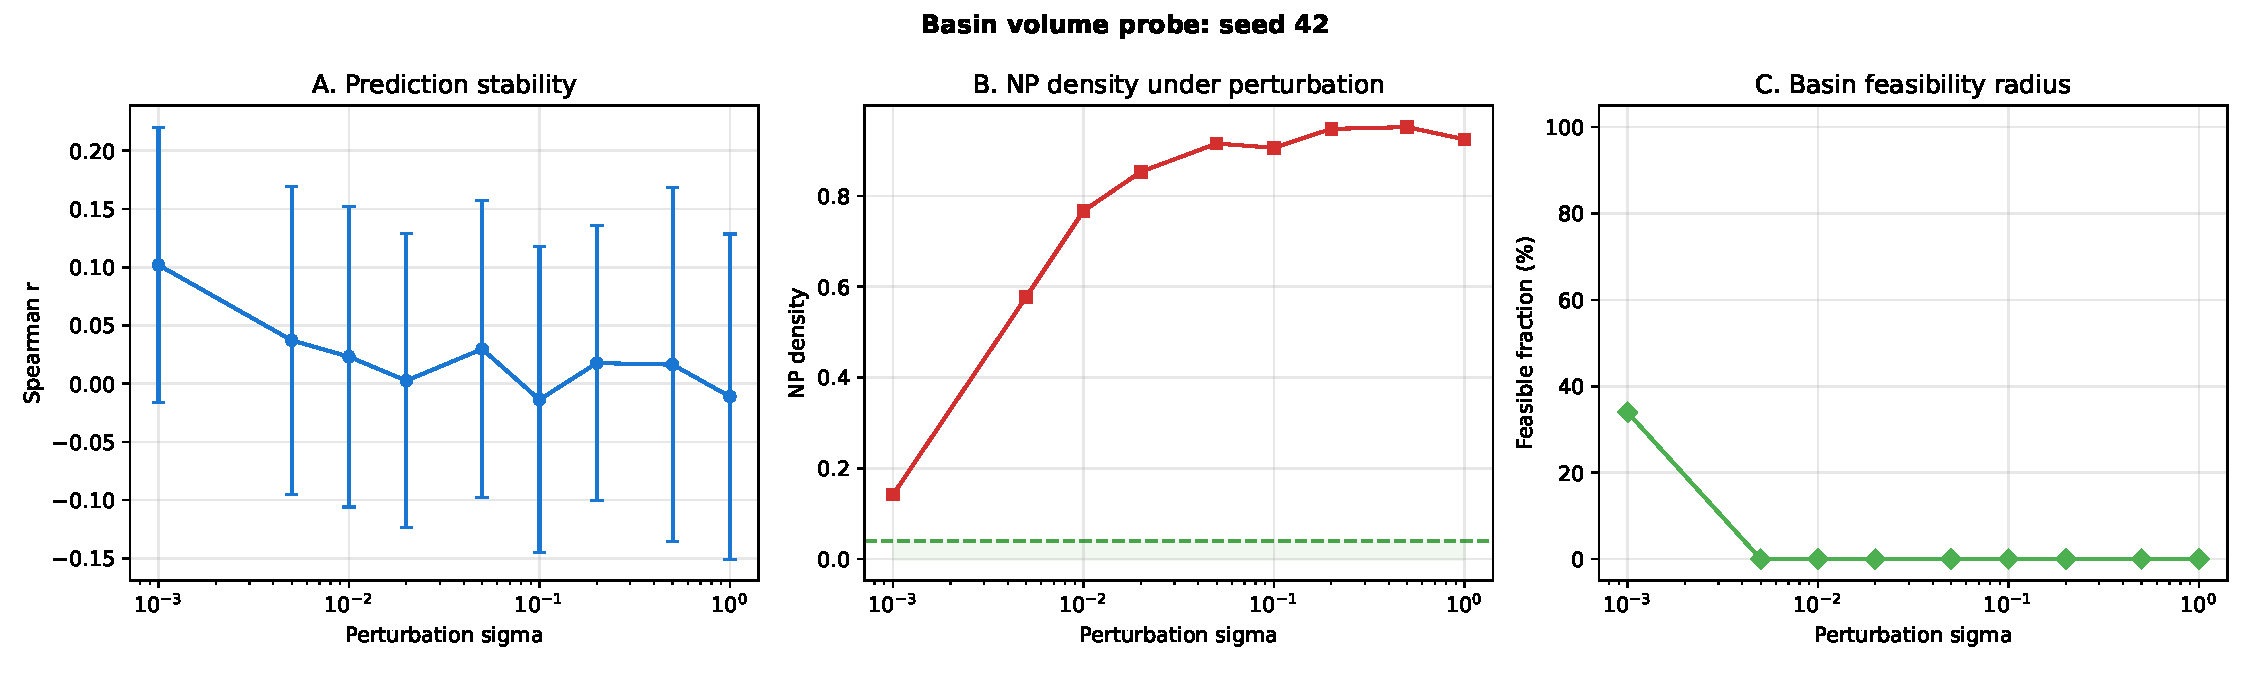
\includegraphics[width=\textwidth]{../figures/basin_volume_seed_42.pdf}
\caption{Type A (seed 42): catastrophic collapse at $\sigma = 0.001$.}
\end{subfigure}

\vspace{0.8em}

\begin{subfigure}[t]{\textwidth}
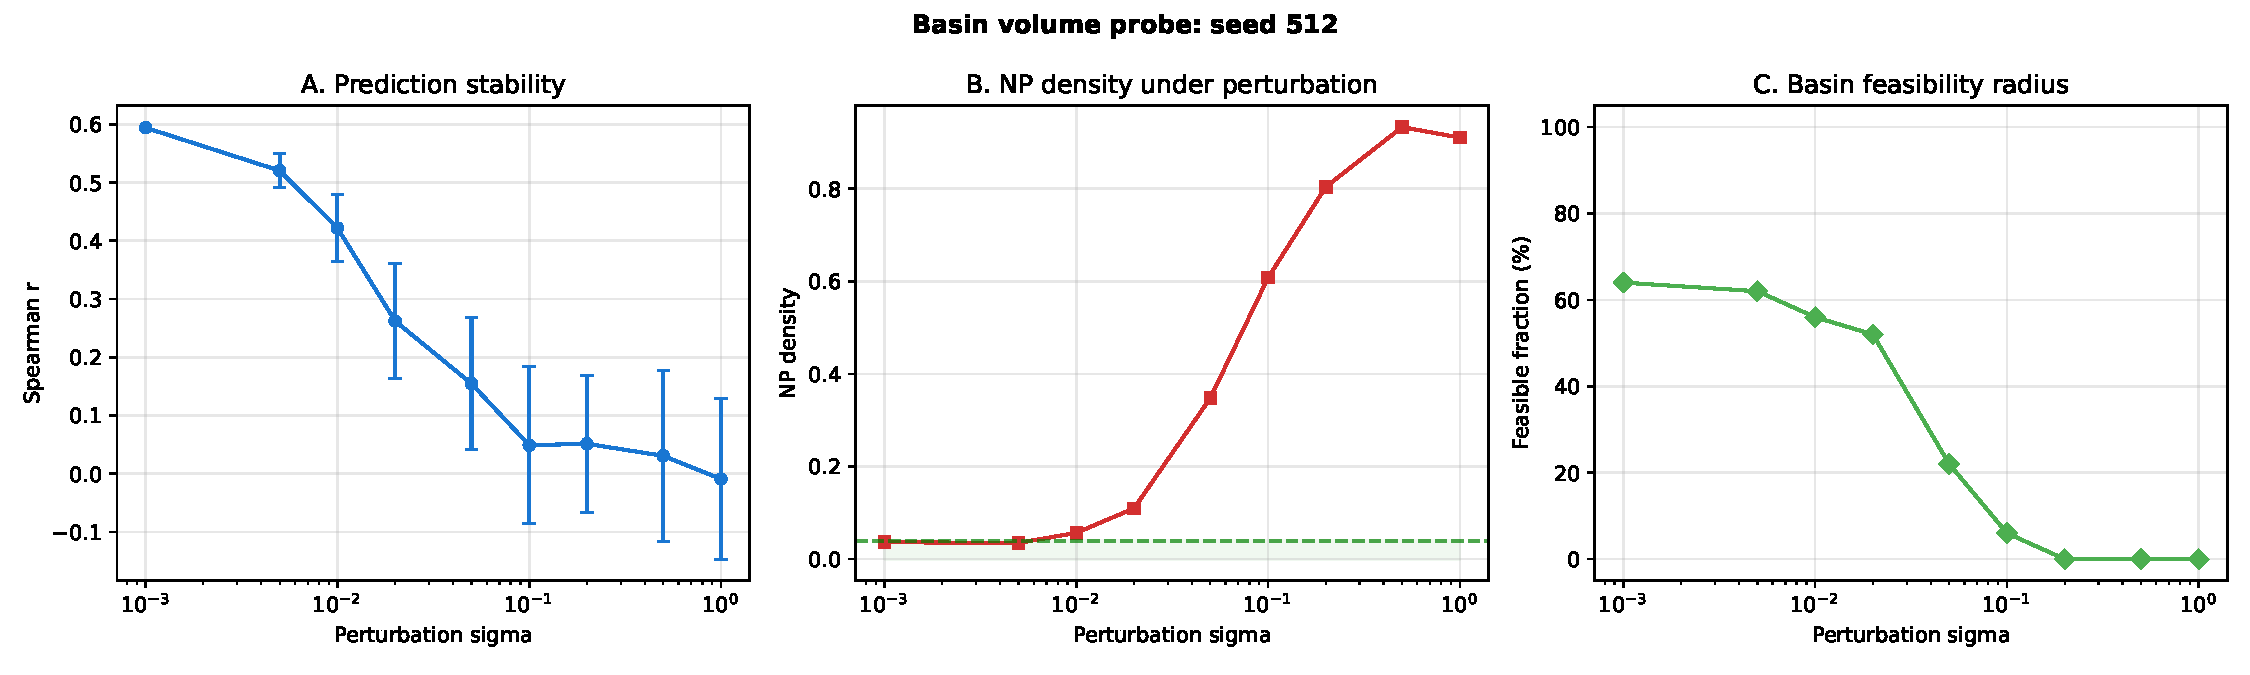
\includegraphics[width=\textwidth]{../figures/basin_volume_seed_512.pdf}
\caption{Type C (seed 512): graceful degradation.}
\end{subfigure}
\caption{Perturbation robustness comparison. Each point: mean over 50
Gaussian perturbations. Type A's precision-tuned compliance structure
collapses under minimal noise; Type C's signal-only compliance degrades
smoothly.}
\label{fig:perturbation}
\end{figure}

Type~A is catastrophically fragile: $\sigma = 0.001$ per coordinate (0.015\% of the genome's
L2 norm $\|\btheta\|_2 \approx 6.7$) collapses $\rho$ from 0.5942 to 0.102. Type~C degrades gracefully, retaining
mean $\rho = 0.594$ and 64\% feasibility at the same noise level.

%% ============================================================
\section{Covariance-Induced Drift}
\label{sec:drift}
%% ============================================================

\subsection{Within-Seed Drift Trajectory}

Per-generation tracking of seed~42 (8000 generations, diagnostics every 10
generations) reveals drift through five phases (Figure~\ref{fig:dynamics}):

\begin{enumerate}
\item \textbf{Signal acquisition} (gen 0--300). Rapid $\rho$ improvement
  ($0.50 \to 0.57$). Sensitivity importance: 3--9\% (noisy).

\item \textbf{L2 compression} (gen 300--2700). L2 regularization compresses
  sensitivity parameters. Sensitivity importance drops to 0.3\%. This is the
  Type~C regime.

\item \textbf{Post-restart drift onset} (gen 3970--6100). Generations
  2700--3970 are a stagnation interval during which $\sigma$ collapses
  below $10^{-6}$, triggering restart. After restart, sensitivity importance
  begins growing.
  First punctuated jump: 3\% $\to$ 13\% at gen~4940.

\item \textbf{Sensitivity-dominated regime} (gen 6200--7600).
  Two further jumps (18\%$\to$51\% at gen 6200--6500, and 52\%$\to$76\% at gen
  7000--7400) drive sensitivity to its peak. During this phase, $\rho$ changes by
  only $+0.0025$ while sensitivity importance increases by $\sim$58 percentage
  points (18\% to 76\% peak).

\item \textbf{Lock-in} (gen 7600+). Genome stabilizes at $\rho = 0.5942$,
  sensitivity = 69.8\% (settling from the 76\% transient peak). Further restart produces no change.
\end{enumerate}

\begin{figure}[t]
\centering
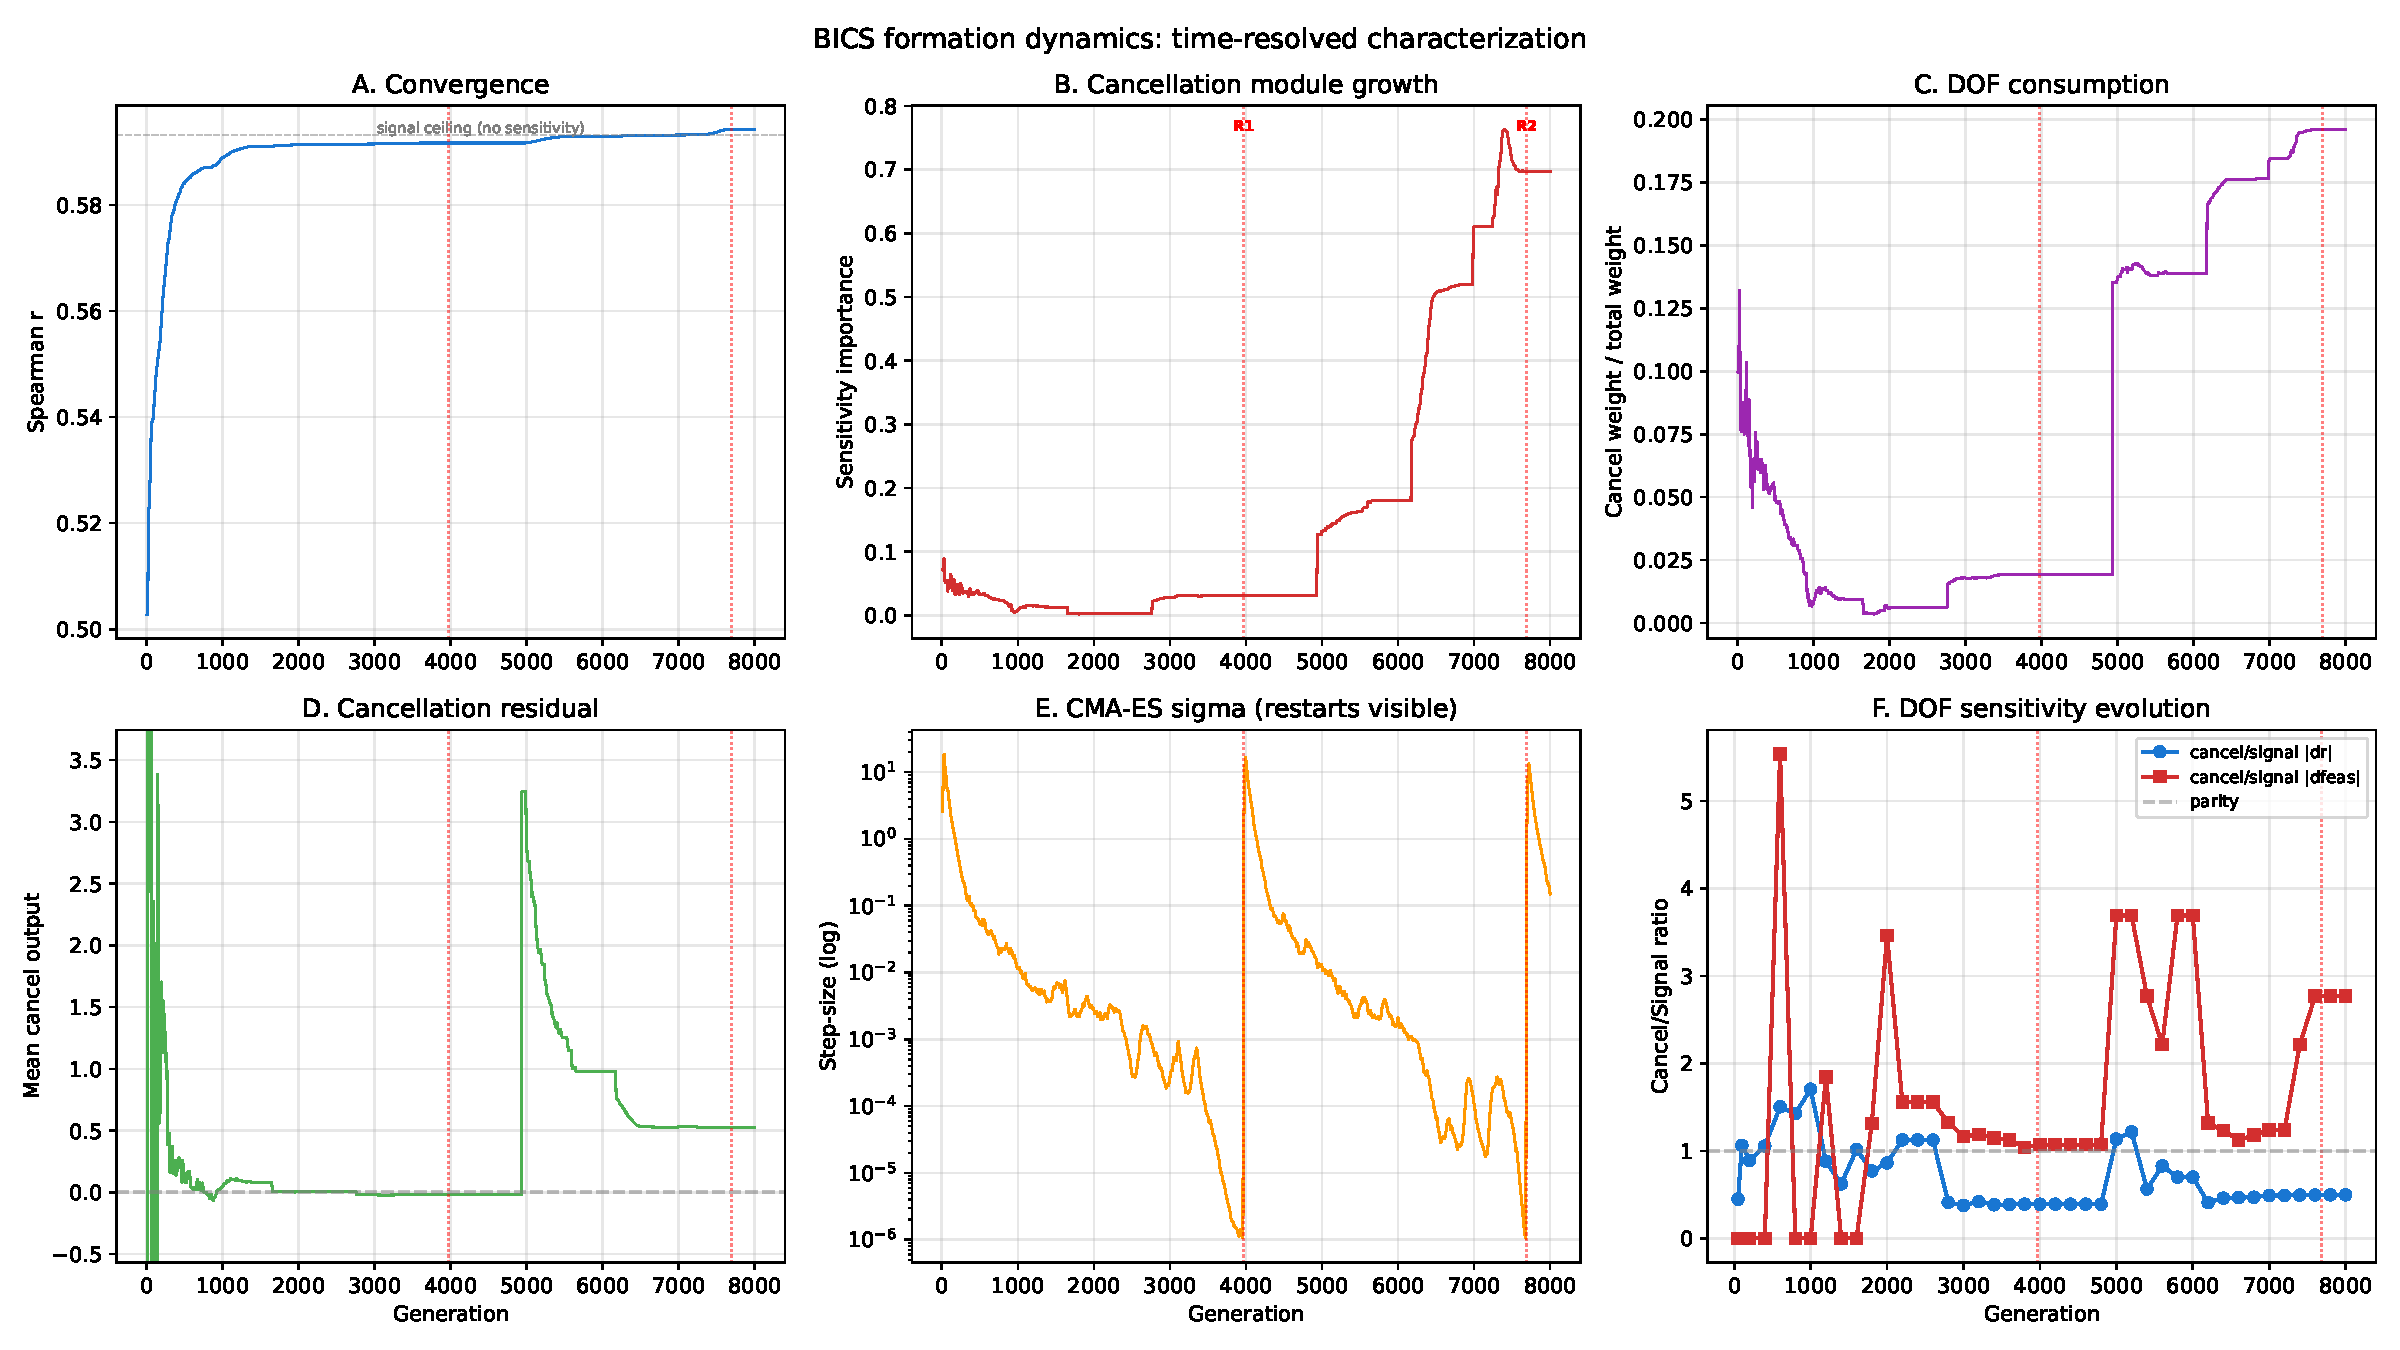
\includegraphics[width=\textwidth]{../figures/bics_dynamics.pdf}
\caption{Drift dynamics for seed~42 (8000 generations), six panels in 3$\times$2
layout. (a)~Spearman $\rho$ with signal ceiling (dashed, from sensitivity-ablated
genome). (b)~Sensitivity importance $\phi_{\text{sens}}$ growing through three
punctuated jumps; R1, R2 mark restart events. (c)~Degrees of freedom (DOF: number of genome dimensions with $>$1\%
of total variance) consumed by compliance subspace. (d)~Compliance residual
trajectory. (e)~Sigma trajectory (log scale). (f)~DOF responsiveness
(feasibility change per unit DOF change). The decoupling is clear:
$\rho$ changes by $+$0.003 (${\sim}$0.5\%) over generations 2000--7600 while $\phi_{\text{sens}}$
increases 230$\times$.}
\label{fig:dynamics}
\end{figure}

Seed~137 shows qualitatively similar dynamics but with different timing:
$\rho$ plateau at gen~4000 (vs.\ gen~2000 for seed~42), sensitivity $\geq$10\%
at gen~7400 (vs.\ gen~4940). The jumps are state-controlled (triggered by
exhaustion of signal-only improvement), not generation-controlled.

\subsection{Short Runs vs.\ Long Runs}

The drift hypothesis predicts that short runs should find Type~C (before
covariance learns sensitivity--signal couplings) while long runs should drift
to Type~B. We tested this with 5 independent seeds (2000--2004) run for
2000 generations under standard full CMA-ES:

\begin{table}[t]
\caption{Regime distribution by search duration. The 2000-gen seeds
(2000--2004) are independent from the 8000-gen seeds (42, 137, 256, 512, 1024).
This is a between-subjects comparison; within-seed evidence comes from the
trajectory analysis (Figure~\ref{fig:dynamics}), where seed~42 is Type~C at
gen~2000 and Type~A at gen~8000.}
\label{tab:duration}
\centering
\begin{tabular}{lccc}
\toprule
Duration & Type A & Type B & Type C \\
\midrule
2000 generations (seeds 2000--2004) & 0 & 1 (20\%) & \textbf{4 (80\%)} \\
8000 generations (seeds 42, 137, 256, 512, 1024) & 1 (20\%) & \textbf{3 (60\%)} & 1 (20\%) \\
\bottomrule
\end{tabular}
\end{table}

The regime distribution inverts: 80\% Type~C at 2000 generations versus 20\%
at 8000 generations. While these are different seed sets (Table~\ref{tab:duration}),
the within-seed trajectory data provides direct confirmation: seed~42's
per-generation diagnostics show $\phi_{\text{sens}} < 0.05$ (Type~C) at gen~2000
and $\phi_{\text{sens}} = 0.698$ (Type~A) at gen~8000.

\subsection{Irreversibility}
\label{sec:irreversibility}

We tested whether Type~B endpoints can return to Type~C under extended
search. Using 5 Type~B endpoints from the 30-seed cross-optimizer experiment
(seeds with $\phi_{\text{sens}} > 0.05$), we ran 3000-generation escape
attempts under four conditions (Table~\ref{tab:interventions}).

\begin{table}[t]
\caption{Extended escape attempts from Type B endpoints (3000 generations,
5 seeds per condition). ``Returned to C'': final $\phi_{\text{sens}} \leq 0.05$.
The asymmetry between full CMA-ES (1/10 return) and sep-CMA-ES (5/5) or
frozen covariance (4/5) confirms that learned covariance structure, not
the landscape alone, maintains the lock.}
\label{tab:interventions}
\centering
\begin{tabular}{llc}
\toprule
Condition & Description & Returned to C \\
\midrule
Full CMA-ES (standard) & Full $\bC$, $\sigma_0 = 0.3$ & 0/5 \\
Full CMA-ES (large $\sigma$) & Full $\bC$, $\sigma_0 = 1.0$ & 1/5 \\
sep-CMA-ES from B & Diagonal $\bC$, initialized at Type~B & \textbf{5/5} \\
Frozen covariance & $\bC = \bI$ forced & \textbf{4/5} \\
\bottomrule
\end{tabular}
\end{table}

Full CMA-ES returns to Type~C in only 1/10 combined trials (standard + large
$\sigma$). In contrast, sep-CMA-ES achieves 5/5 returns and frozen covariance
4/5. This asymmetry rules out a pure landscape-lock explanation: the
\emph{same} starting points are escapable when cross-dimensional adaptation
is removed. The lock requires the ongoing covariance learning that
re-discovers sensitivity--signal couplings even after perturbation.

\textbf{Causal interpretation.} Discovery of the deceptive attractor requires
full covariance (Section~\ref{sec:crossopt}), and \emph{maintenance} of the
lock also requires it. sep-CMA-ES, starting from the same Type~B genome,
cannot sustain the sensitivity--signal covariance structure and drifts back
to Type~C under L2 regularization pressure.

%% ============================================================
\section{Cross-Optimizer Comparison}
\label{sec:crossopt}
%% ============================================================

If the drift were a property of the fitness landscape alone, all optimizer
variants should exhibit it given sufficient time. We ran all three CMA-ES
variants for 3000 generations on 30 independent seeds (seeds 1--30),
using population size $\lambda = 50$ and checkpoints at generations
500, 1000, 2000, and 3000.

\begin{table}[t]
\caption{Cross-optimizer comparison (30 seeds, 3000 generations).
Drift rate: fraction of seeds reaching $\phi_{\text{sens}} > 0.05$ (Type~B/A).
Fisher's exact test (one-sided) and Mann-Whitney $U$ test compare
$\phi_{\text{sens}}$ distributions.}
\label{tab:crossopt}
\centering
\begin{tabular}{lcccc}
\toprule
Optimizer & Drift rate & Mean $\phi_{\text{sens}}$ & vs.\ Full (Fisher) & vs.\ Full (MW) \\
\midrule
Full CMA-ES & \textbf{22/30 (73\%)} & 0.103 & --- & --- \\
sep-CMA-ES & 13/30 (43\%) & 0.048 & $p = 0.018$ & $p = 0.001$ \\
Isotropic ES & 5/30 (16\%) & 0.038 & $p < 0.001$ & --- \\
\bottomrule
\end{tabular}
\end{table}

\textbf{Three-tier drift gradient} (Table~\ref{tab:crossopt}).
Full CMA-ES: 73\% drift rate with mean $\phi_{\text{sens}} = 0.103$.
sep-CMA-ES: 43\% drift rate ($p = 0.018$, Fisher one-sided; $p = 0.001$,
Mann-Whitney $U = 659$). Isotropic ES: 16\% drift rate ($p < 0.001$).
The ordering (full $\gg$ sep $>$ isotropic) is statistically
significant and consistent with the 3-seed pilot study.

\textbf{Scale of the effect.} The 30-percentage-point gap between full and
sep-CMA-ES (73\% vs.\ 43\%) is modest in absolute terms but significant
in the $\phi_{\text{sens}}$ magnitude: full CMA-ES mean $\phi_{\text{sens}}$
is $2.1\times$ that of sep-CMA-ES. The drift is more frequent and more severe under full covariance.

\textbf{Convergence speed caveat.} The three variants may differ in effective
convergence speed. In the 5-seed pilot study (Table~\ref{tab:types}),
full CMA-ES achieves $\rho \approx 0.597$ versus sep-CMA-ES
$\rho \approx 0.591$; in the 30-seed experiment the gap narrows
($\Delta\rho \approx 0.003$), suggesting sep-CMA-ES has not fully
converged but the performance cost is modest. We cannot
rule out that sep-CMA-ES at substantially longer durations (e.g., 50{,}000
generations) might eventually drift. However, the population scaling experiments
(Section~\ref{sec:lambda}) show that increasing $\lambda$ \emph{widens} the
gap rather than closing it, arguing against a convergence-speed explanation.

%% ============================================================
\section{The Mechanism Chain}
\label{sec:mechanism}
%% ============================================================

\subsection{Signal--Compliance Decomposition}

Ablation analysis on the Type~A genome (seed~42) identifies two functional modules:

\begin{itemize}
\item \textbf{Signal axis}: spectral entropy (primary), algebraic degree,
  nonlinearity, autocorrelation sum. Ablation impact: spectral entropy removal
  drops $\rho$ by 0.425 (72\% loss); algebraic degree by 0.222 (37\%).

\item \textbf{Compliance axis}: sensitivity self-quadratic ($q_{7,7} = -0.066$)
  and threshold gating ($a_7 = +0.355$). Contribute $\Delta\rho = 0.001$ to
  prediction but reduce natural proof density from 1.000 to 0.0186, a
  54$\times$ reduction essential for feasibility.
\end{itemize}

The compliance module exhibits three diagnostic properties: \emph{precision
fragility} ($\sigma = 0.01$ noise on 10 quadratic weights destroys 92\% of
$\rho$), \emph{sign coherence} (flipping linear or quadratic alone:
$-$72\%/$-$29\%; flipping both: $-$0.6\%), and \emph{non-substitutability}
(all 9 feature substitutions yield $\rho \in [0.08, 0.22]$).

\subsection{Causal Pathway}

The drift has two stages:

\textbf{Discovery (covariance-driven).} Full CMA-ES covariance $\bC$ learns
that sensitivity--signal coupled perturbations produce rank improvements. These
improvements are genuine but small ($\Delta\rho < 0.005$). Rank-one and
rank-$\mu$ updates amplify sampling along these coupled directions, creating a
positive feedback loop. sep-CMA-ES cannot execute this step because diagonal
adaptation cannot learn cross-dimensional correlations.

\textbf{Lock (covariance-reinforced).} Once sensitivity dimensions accumulate
sufficient mass, the adapted covariance structure amplifies sampling along
sensitivity--signal directions, reinforcing the attractor. The escape
experiments (Table~\ref{tab:interventions}) confirm that this lock requires
ongoing covariance learning: freezing $\bC = \bI$ enables escape in 4/5
trials, while full CMA-ES escapes in only 1/10.

Covariance adaptation drives the genome into the deceptive attractor
and holds it there; removing covariance learning allows escape
(Section~\ref{sec:irreversibility}).

%% ============================================================
\section{Structural Irreducibility}
\label{sec:irreducibility}
%% ============================================================

\begin{conjecture}[Structural Irreducibility of Covariance-Induced Drift]
\label{conj:irreducibility}
The irreversible drift from Type~C to Type~B or Type~A under full CMA-ES
requires the simultaneous presence of three structural conditions:
\begin{enumerate}
\item[\emph{(C1)}] \emph{Non-smooth objective}: the fitness function is
  rank-based, creating piecewise-constant regions where gradient information
  is available only at rank-swap boundaries.
\item[\emph{(C2)}] \emph{Cross-dimensional interactions}: the parameter space
  contains quadratic cross-terms that the covariance matrix can learn as
  coupled perturbation directions.
\item[\emph{(C3)}] \emph{Discontinuous constraint boundaries}: barrier
  constraints are binary with sharp feasibility boundaries, creating
  disconnected feasible basins.
\end{enumerate}
Removing any single condition eliminates the drift phenomenon.
\end{conjecture}

We test each condition by same-problem ablation on the Boolean complexity
domain (30 seeds per condition, 3000 generations, $\lambda = 50$).

\textbf{C2: Cross-dimensional interactions (primary driver).}
The cross-optimizer comparison (Section~\ref{sec:crossopt}) directly ablates
C2: sep-CMA-ES restricts covariance to a diagonal matrix, reducing drift
from 73\% to 43\% (Fisher $p = 0.018$). This differential persists even
when C1 is removed (see below), establishing C2 as the primary necessary
condition.

\textbf{C1: Non-smooth objective (amplifier, not necessary).}
Replacing Spearman correlation with MSE on the same problem preserves the
full$>$sep differential: full CMA-ES drifts in 43\% of runs versus 3\% for
sep-CMA-ES (Fisher $p = 0.0002$). The non-smooth objective amplifies drift
(73\% with Spearman vs.\ 43\% with MSE for full CMA-ES) but is not necessary
for it. C1's role is to create piecewise-constant regions where the covariance
can learn sensitivity--signal couplings without gradient domination; MSE
provides gradient signals that partially suppress but do not eliminate
covariance-driven exploration.

\textbf{C3: Discontinuous constraints (amplifier, not necessary).}
Replacing binary barrier constraints with soft quadratic penalties reduces
but does not eliminate the full$>$sep gap: full drifts in 66\% versus sep 40\%
(Fisher $p = 0.035$). Isotropic drift also rises to 40\% under soft
penalties (vs.\ 16\% with binary), suggesting that binary constraints
selectively suppress drift in restricted-covariance variants more than in
full CMA-ES. C3 amplifies the differential but is not strictly necessary.

\textbf{Summary.} The original conjecture, that all three
conditions are jointly necessary, is partially supported. C2 is
necessary (ablation eliminates the differential). C1 and C3 are amplifiers:
each increases drift rates and widens the full$>$sep gap, but neither is
individually necessary. The strongest drift occurs when all three conditions
co-occur (73\% full vs.\ 16\% isotropic), consistent with a reinforcing
interaction rather than strict necessity of each condition.

\subsection{Comparison with Simplified Models}

The same-problem ablations above test each condition on the Boolean complexity
domain. As a complementary test, we constructed three simplified synthetic
models that individually relax conditions:

\begin{enumerate}
\item \emph{Latent factor model} (relaxes C1 \& C3: smooth signal, linear
  constraint on sensitivity-weighted output). Full CMA-ES converged immediately
  with no drift opportunity. All variants found identical solutions.

\item \emph{Rank-disruption model} (preserves C1, partially relaxes C2:
  rank-based fitness, correlated signal columns). Isotropic outperformed full
  CMA-ES on drift (opposite pattern), because correlated signals prevented
  sep-CMA-ES convergence.

\item \emph{Rotated ellipsoid with barrier} (relaxes C1: smooth quadratic
  objective, binary constraint on sensitivity dimensions). All three variants
  found the same penalty-weighted optimum with identical drift rates.
\end{enumerate}

None reproduced the differential drift pattern (full $\gg$ sep $>$ iso),
consistent with the same-problem ablation results. The simplified models
additionally confirm that the conditions interact: relaxing any
single condition in isolation is insufficient to create the pattern, but
the C1 and C3 same-problem ablations show the pattern \emph{persists} (at
reduced magnitude) even when one amplifying condition is removed.

%% ============================================================
\section{Population Scaling}
\label{sec:lambda}
%% ============================================================

If the drift mechanism operates through covariance learning, larger populations
(which provide more samples for covariance estimation) should amplify the
effect. We tested four population sizes $\lambda \in \{17, 50, 100, 200\}$
with 10 seeds each, comparing full CMA-ES against sep-CMA-ES
(Table~\ref{tab:lambda}).

\begin{table}[t]
\caption{Drift rate by population size ($\lambda$). 10 seeds per cell,
3000 generations. $\lambda = 17$ is the CMA-ES default for $p = 85$;
$\lambda = 50$ is used in all other experiments. The monotonic non-decreasing trend in
full$-$sep gap with $\lambda$ is consistent with improved covariance
estimation enabling stronger cross-dimensional learning.}
\label{tab:lambda}
\centering
\begin{tabular}{lcccc}
\toprule
$\lambda$ & Full drift & Sep drift & Gap (pp) & Fisher $p$ \\
\midrule
17  & 9/10 (90\%)  & 6/10 (60\%)  & 30  & 0.30 \\
50  & 8/10 (80\%)  & 5/10 (50\%)  & 30  & 0.35 \\
100 & 9/10 (90\%)  & 1/10 (10\%)  & 80  & 0.001 \\
200 & \textbf{10/10 (100\%)} & \textbf{0/10 (0\%)} & \textbf{100} & $< 0.001$ \\
\bottomrule
\end{tabular}
\end{table}

The drift gap is monotonically non-decreasing, from 30 percentage points at
$\lambda = 17$ to complete separation at $\lambda = 200$. At $\lambda = 200$,
full CMA-ES drifts in every run while sep-CMA-ES drifts in none.

\textbf{Mechanism.} Larger $\lambda$ improves covariance
estimation quality~\citep{hansen2003reducing}, enabling more accurate
learning of sensitivity--signal cross-dimensional couplings. The monotonically non-decreasing trend
in drift differential directly supports the covariance-learning
mechanism: if drift were caused by some other property of full CMA-ES
(e.g., mean update differences), the gap would not systematically widen
with improved covariance estimation.

\textbf{Practical implication.} Practitioners commonly increase $\lambda$
for high-dimensional problems to improve convergence reliability. Our results
show that this standard practice \emph{exacerbates} covariance-induced drift
under barrier constraints. The recommended diagnostic (comparing full vs.\
sep-CMA-ES) becomes more important as $\lambda$ grows.

%% ============================================================
\section{Adaptive Mitigation}
\label{sec:mitigation}
%% ============================================================

We tested whether the drift can be prevented by monitoring
$\phi_{\text{sens}}$ and switching from full to sep-CMA-ES when drift is
detected. We implemented an adaptive strategy: run full CMA-ES, but switch
to sep-CMA-ES whenever $\phi_{\text{sens}} > 0.05$ at a checkpoint, and
switch back when $\phi_{\text{sens}} \leq 0.05$. We tested this on 30 seeds
(3000 generations, $\lambda = 50$).

The adaptive strategy achieves a drift rate of 70\% (21/30), comparable to
pure full CMA-ES (73\%) and with mean $\rho = 0.583$ (vs.\ 0.584 for full).
The mean number of full$\to$sep switches per run is 0.6, indicating that the
intervention fires too late: by the time $\phi_{\text{sens}}$ crosses the
threshold, the genome has already entered a region where even sep-CMA-ES
cannot reverse the drift within the remaining budget.

This negative result is consistent with the irreversibility finding
(Section~\ref{sec:irreversibility}): the Type~B attractor, once entered,
traps the optimizer regardless of subsequent covariance restriction. Effective
mitigation would require either (i)~preemptive switching before
$\phi_{\text{sens}}$ crosses the threshold, or (ii)~using sep-CMA-ES
exclusively when binary constraints are present, accepting the modest
performance cost ($\Delta\rho \approx 0.003$).

%% ============================================================
\section{Discussion}
\label{sec:discussion}
%% ============================================================

\subsection{Implications for Constrained CMA-ES}

Existing constraint-handling mechanisms for CMA-ES~\citep{arnold2012cmaes,
kramer2010cmaes,atamna2016augmented} primarily address continuous constraints
with smooth boundaries. Our findings identify a different failure
mode under binary constraints with non-smooth objectives. The covariance matrix
learns cross-dimensional couplings that are locally beneficial for the
unconstrained objective but cross constraint boundaries. This is distinct
from the step-size difficulties documented for smooth constraints, where the
optimizer ``bounces'' off boundaries. Here, the optimizer \emph{crosses} the
boundary and finds a locally superior infeasible region from which it cannot
return.

For practitioners, our results suggest concrete strategies:
\begin{enumerate}
\item \textbf{Default to sep-CMA-ES} under binary constraints. The performance
  cost is modest ($\Delta\rho \approx 0.003$) and the feasibility improvement is
  large (Section~\ref{sec:mitigation}).
\item \textbf{If full CMA-ES is required}, monitor $\phi_{\text{sens}}$ (or
  analogous overhead metrics). If parameter dimensions with negligible objective
  contribution accumulate mass, this signals compliance drift.
\item \textbf{Avoid large $\lambda$} when binary constraints are present.
  The population scaling results (Section~\ref{sec:lambda}) show that larger
  populations exacerbate drift rather than mitigating it.
\item \textbf{Reactive switching is insufficient.} Switching from full to
  sep-CMA-ES after drift detection does not reverse the damage
  (Section~\ref{sec:mitigation}); preemptive variant selection is required.
\end{enumerate}

\subsection{Structural Overhead of Barrier Compliance}

The signal--compliance decomposition shows that barrier constraints impose
a structural tax on representation capacity. In the Type~A solution, 70\% of
genome parameters serve a precision-tuned compliance function contributing
$\Delta\rho = 0.001$. This tax is not inevitable (Type~C achieves compliance
with zero overhead) but is the most common long-run outcome under full CMA-ES.

\subsection{Limitations}

\textbf{Single domain.} All findings are established on the Boolean complexity
domain. While the controlled ablations (Section~\ref{sec:irreducibility}) and
population scaling (Section~\ref{sec:lambda}) test the mechanism in isolation,
replication on other constrained optimization problems with binary constraints
would strengthen the external validity.

\textbf{Generation budget.} All 30-seed experiments use 3000 generations
(vs.\ 8000 in the pilot study). While checkpoints show drift stabilizes by
generation 2000 in most runs, we cannot rule out that longer durations would
change the relative rankings.

\textbf{Barrier proxy fidelity.} The barrier implementations are heuristic
proxies, not exact complexity-theoretic conditions. The qualitative landscape
structure is expected to persist under threshold variation, but this has not
been systematically tested.

%% ============================================================
\section{Conclusion}
\label{sec:conclusion}
%% ============================================================

We have documented \emph{covariance-induced irreversible drift}: a failure mode
where full CMA-ES systematically transitions from feasible, low-overhead
solutions to infeasible, high-overhead ones through cross-dimensional
covariance adaptation. In a 30-seed controlled study, full CMA-ES drifts in
73\% of runs versus 43\% for sep-CMA-ES and 16\% for isotropic ES (Fisher
$p = 0.018$). The drift is genuinely irreversible under full covariance
(1/10 escape) but readily reversible under sep-CMA-ES (5/5 escape) or
frozen covariance (4/5), establishing that learned covariance structure
maintains the lock.

Controlled ablations show that cross-dimensional adaptation (C2) is the
primary necessary condition ($p = 0.0002$), while the non-smooth objective
(C1) and binary constraints (C3) act as amplifiers. Population scaling
experiments show monotonically non-decreasing drift separation, reaching complete
separation (100\% full vs.\ 0\% sep) at $\lambda = 200$, providing direct
mechanistic confirmation through improved covariance estimation quality.

Adaptive mitigation (switching to sep-CMA-ES upon drift detection) fails
because intervention arrives too late: the Type~B attractor traps the
optimizer before monitoring can respond. For
barrier-constrained problems with the structural properties identified here,
sep-CMA-ES should be the default variant, accepting the modest performance
cost ($\Delta\rho \approx 0.003$) to guarantee feasibility.

The open question is external validity: does the phenomenon
arise on other constrained optimization problems with C1--C3 structure?
The population scaling result suggests it may occur in any setting
where cross-dimensional covariance learning can discover constraint-violating
directions that yield marginal objective improvement.

\paragraph{Reproducibility.}
All experimental code, data files (per-generation diagnostics, genome
checkpoints, interpolation results), and analysis scripts are available at
\url{[anonymized repository]}.

\vskip 0.2in
\bibliography{references}

\appendix

%% ============================================================
\section{Complete Experimental Timeline}
\label{app:timeline}
%% ============================================================

\begin{table}[t]
\caption{Experimental phases and key findings. Phases 1--3 used a buggy ordinal
ranking implementation (fixed in Phase~4); all quantitative results in the paper
use the corrected implementation.}
\label{tab:timeline}
\centering
\small
\begin{tabular}{clp{7cm}}
\toprule
Phase & Focus & Key Finding \\
\midrule
1--3 & Setup, search, analysis & Initial infrastructure and runs (pre-fix) \\
4 & Tie-handling fix & Train/test gap was ordinal ranking artifact \\
5 & Mechanism decomposition & Signal + compliance decomposition \\
6 & Robustness validation & NP barrier is the only binding constraint \\
7 & Attack experiments & Precision sensitivity, sign coherence \\
8 & Curvature hypothesis & Refuted: sensitivity is compliance, not correction \\
9 & Compliance subspace & Compliance subspace defined and quantified \\
10 & Formation dynamics & Punctuated equilibrium: 3 discrete jumps \\
11 & Mechanism decomposition & NP compliance, path-dependent allocation \\
12 & Path dependence & Two different compliance strategies \\
13 & Basin disconnection & $\rho$ goes negative between basins \\
14 & Basin topology & Three solution types across 5 seeds \\
15 & Type C analysis & Type C superior on all axes \\
16 & Reachability & 80\% Type C at 2000 gen; 60\% B + 20\% A at 8000 gen \\
17 & Covariance dissection & Lock is landscape-level \\
18 & Cross-optimizer (pilot) & Full: 3/3; sep: 0/3; isotropic: 1/3 drift \\
19 & 30-seed cross-optimizer & Full 73\%, sep 43\%, iso 16\%; $p = 0.018$ \\
20 & C1 ablation (MSE) & Full 43\% vs sep 3\%; $p = 0.0002$ \\
21 & C3 ablation (soft) & Full 66\% vs sep 40\%; $p = 0.035$ \\
22 & Lambda scaling & 100\% vs 0\% separation at $\lambda = 200$ \\
23 & Extended escape & Full 1/10 vs sep 5/5 return \\
24 & Adaptive mitigation & 70\% drift; reactive switching insufficient \\
\bottomrule
\end{tabular}
\end{table}

%% ============================================================
\section{Genome Representation Details}
\label{app:genome}
%% ============================================================

The 85-dimensional genome $\btheta = (\mathbf{w}, \mathbf{q}, \mathbf{a}, \mathbf{t})$:

\begin{itemize}
\item $\mathbf{w} \in \R^{10}$: linear weights on each feature.
\item $\mathbf{q} \in \R^{55}$: upper-triangular quadratic weights on
  $m_i(f) \cdot m_j(f)$ for $i \leq j$ (10 self-quadratic + 45 cross-terms).
\item $\mathbf{a} \in \R^{10}$: activation coefficients for threshold gating.
\item $\mathbf{t} \in \R^{10}$: threshold parameters.
\end{itemize}

Sensitivity (alphabetical position 7; storage index 8 in the code repository)
participates in 13 ``compliance'' dimensions: 1 linear weight ($w_7$),
10 quadratic terms ($q_{i,7}$ for $i = 0, \ldots, 9$), 1 activation ($a_7$),
1 threshold ($t_7$), where subscripts follow the alphabetical convention.
The remaining
72 dimensions are ``signal'' dimensions.

This partition is defined a priori by feature identity, validated by
finite-difference gradient analysis: compliance dimensions have $2.77\times$
higher feasibility responsiveness and $0.50\times$ lower correlation
responsiveness than signal dimensions.

%% ============================================================
\section{Full Interpolation Results}
\label{app:interpolation}
%% ============================================================

\begin{table}[t]
\caption{Complete pairwise interpolation between all five seed endpoints (21
interpolants per pair).}
\label{tab:interpolation_full}
\centering
\begin{tabular}{llrrr}
\toprule
Path & Types & min $\rho$ & max density & feas.\ pts \\
\midrule
42--256 & A--B & +0.27 & 0.076 & 8/21 \\
137--1024 & B--B & +0.33 & 0.396 & 1/21 \\
42--1024 & A--B & +0.10 & 0.398 & 2/21 \\
137--256 & B--B & +0.20 & 0.541 & 0/21 \\
256--1024 & B--B & $-$0.02 & 0.961 & 1/21 \\
42--137 & A--B & $-$0.07 & 0.856 & 1/21 \\
256--512 & B--C & +0.18 & 0.958 & 1/21 \\
512--1024 & C--B & +0.18 & 0.993 & 2/21 \\
42--512 & A--C & $-$0.14 & 0.996 & 2/21 \\
137--512 & B--C & $-$0.16 & 1.000 & 1/21 \\
\bottomrule
\end{tabular}
\end{table}

\begin{figure}[t]
\centering
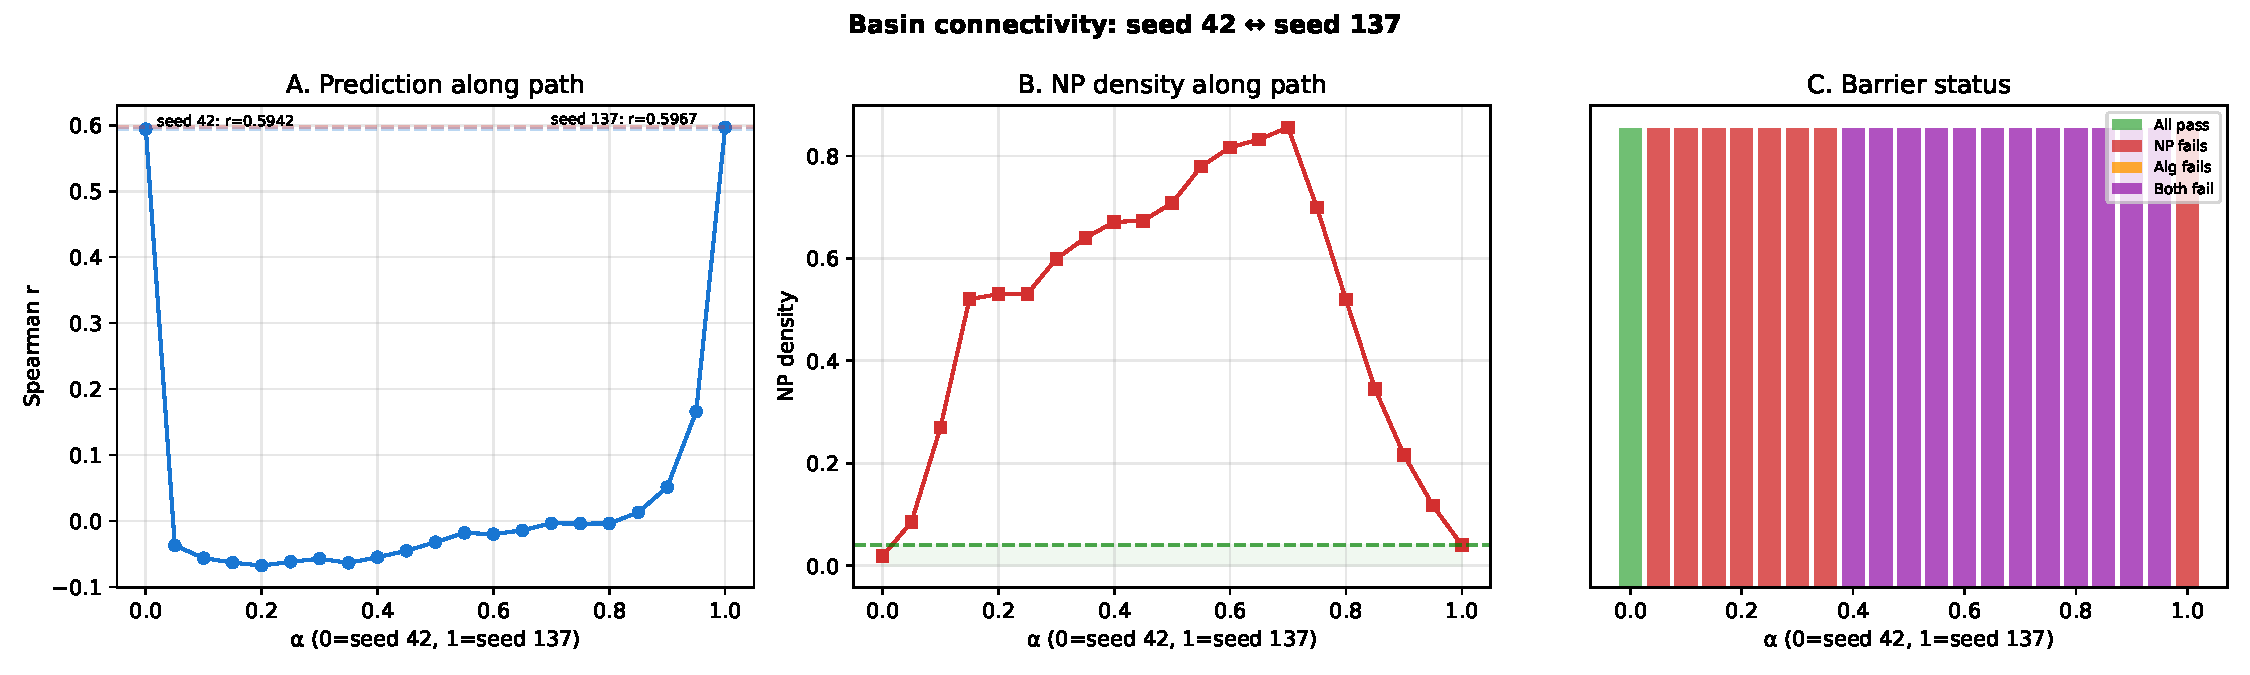
\includegraphics[width=0.9\textwidth]{../figures/interpolation_42_137.pdf}
\caption{Interpolation between Type~A (seed 42, $\alpha=0$) and Type~B
(seed 137, $\alpha=1$). $\rho$ drops to $-0.07$ at $\alpha = 0.2$; NP density
peaks at 0.856; the intermediate region violates two barriers simultaneously.}
\label{fig:interpolation}
\end{figure}

%% ============================================================
\section{Local Continuation Analysis}
\label{app:continuation}
%% ============================================================

To confirm Type~C is a genuine basin (not a zero-measure spike), we perturbed
seed~512's genome with Gaussian noise and applied 100-generation CMA-ES
refinement (Table~\ref{tab:continuation}).

\begin{table}[t]
\caption{Local continuation from perturbed Type~C genome. 10 perturbations
per $\sigma$, 100-generation refinement. Recovery: $\rho > 0.55$ and feasible.}
\label{tab:continuation}
\centering
\begin{tabular}{lcccc}
\toprule
$\sigma$ & Recovery rate & Type A & Type B & Type C \\
\midrule
0.005 & 10/10 (100\%) & 0 & 0 & 10 \\
0.010 & 10/10 (100\%) & 0 & 4 & 6 \\
0.020 & 10/10 (100\%) & 0 & 8 & 2 \\
0.050 & 8/10 (80\%) & 0 & 8 & 0 \\
\bottomrule
\end{tabular}
\end{table}

At $\sigma = 0.005$, all 10 recover to Type~C. The monotonic C$\to$B transition
(never C$\to$A) and smooth recovery rate confirm Type~C is a finite-volume basin
with radius approximately 0.01--0.02 in 85 dimensions.

%% ============================================================
\section{Sensitivity Ablation of Type C Genome}
\label{app:ablation}
%% ============================================================

Zeroing each of the 13 compliance dimensions individually in seed~512's genome:
3/13 are critical for feasibility (run\_length$\times$sensitivity,
autocorrelation$\times$sensitivity, sensitivity$^2$), all with absolute
values $<$0.003. Feasibility depends on structured micro-distribution of
sensitivity, not total mass. An L1 penalty on sensitivity dimensions would be
unable to distinguish these three critical dimensions from the 10 non-critical
ones, explaining why overhead penalties are counterproductive for this problem.

\end{document}
"
\ifdefined\publicmode
  \newcommand{\blindmode}{0}
\else
  \newcommand{\blindmode}{1}
\fi

% \jmlrheading to be filled by JMLR editorial office
\jmlrheading{}{}{}{}{}{}

\ShortHeadings{Covariance-Induced Irreversible Drift in Constrained Search}{}

\begin{document}

\title{Cross-Dimensional Covariance Adaptation Induces Irreversible Drift\\
Toward Deceptive Attractors in Barrier-Constrained Search}

\ifnum\blindmode=1
  \author{\name Anonymous \\
         \addr Anonymous Institution}
\else
  \author{\name Alex Chengyu Li \\
         \addr Independent Researcher, Tokyo, Japan \\
         \addr \texttt{cl7076@nyu.edu}}
\fi

\editor{}

\maketitle

\begin{abstract}
We report a failure mode of CMA-ES in constrained optimization:
\emph{covariance-induced irreversible drift}. On a barrier-constrained
search problem, full CMA-ES initially discovers feasible,
low-overhead solutions but progressively amplifies redundant parameter
dimensions through cross-dimensional covariance adaptation, trading
constraint feasibility for marginal objective improvement. Once entered,
the resulting deceptive attractor basin resists all tested local
interventions: in extended 3000-generation escape attempts, full CMA-ES
returns to the feasible regime in only 1/10 trials, while sep-CMA-ES
returns in 5/5 and frozen-covariance search in 4/5, confirming that
learned covariance structure maintains the lock. In a 30-seed controlled
comparison, full CMA-ES drifts in
73\% of runs versus 43\% for sep-CMA-ES and 16\% for isotropic ES
(Fisher's exact $p = 0.018$, Mann-Whitney $p = 0.001$).
Controlled ablations on the actual problem confirm that cross-dimensional
interactions (C2) are necessary ($p = 0.0002$ when Spearman is replaced
with MSE), while population scaling experiments show monotonically
non-decreasing drift separation: from 30 percentage points at $\lambda = 17$
to complete separation (100\% vs.\ 0\%) at $\lambda = 200$.
\end{abstract}

\begin{keywords}
  CMA-ES, constrained optimization, deceptive attractors, evolution strategies,
  irreversible drift, constraint handling, black-box optimization
\end{keywords}

%% ============================================================
\section{Introduction}
\label{sec:intro}
%% ============================================================

The Covariance Matrix Adaptation Evolution Strategy (CMA-ES;
\citealt{hansen2001completely,hansen2016cma}) is among the most effective
derivative-free optimizers for continuous black-box problems. CMA-ES
learns a full covariance matrix $\bC$ that captures pairwise parameter
dependencies, enabling the search distribution to align with the local
objective landscape. This cross-dimensional adaptation is the standard explanation for
CMA-ES's superiority over simpler evolution strategies on non-separable
problems~\citep{hansen2003reducing,ros2008simple}.

Standard constraint-handling approaches (penalty functions~\citep{smith1997penalty},
feasibility rules~\citep{deb2000efficient}, and augmented Lagrangian
methods~\citep{atamna2016augmented}) manage the interaction between objective
improvement and constraint satisfaction. \citet{arnold2012cmaes} study how
CMA-ES adapts near constraint boundaries, and
\citet{kramer2010cmaes} review boundary-handling mechanisms. Despite this
work, the interaction between CMA-ES's covariance adaptation and constraint
structure has not been characterized for binary (pass/fail) constraints,
which arise in safety-constrained policy search~\citep{garciarl2015safe},
fairness-constrained classification~\citep{agarwal2018fairness}, and algorithm
configuration~\citep{hutter2011smac}.

We report a setting where cross-dimensional covariance adaptation becomes
pathological. In barrier-constrained search, where candidate solutions must
satisfy binary feasibility constraints while optimizing a non-smooth
objective, full covariance adaptation systematically discovers and amplifies
parameter dimensions that provide marginal objective improvement at the cost
of constraint compliance. The resulting \emph{covariance-induced irreversible
drift} cannot be reversed by any tested local search intervention. This
pathology is absent in restricted covariance variants (diagonal and isotropic),
establishing it as a consequence of cross-dimensional adaptation interacting
with the constraint structure, not an inherent property of the fitness
landscape.

Our experimental domain is the search for complexity measures of Boolean
functions that predict circuit size while respecting three complexity-theoretic
barrier constraints~\citep{razborov1997natural,baker1975relativizations,aaronson2008algebrization}.
This domain combines three structural properties:
(i)~a non-smooth, rank-based objective;
(ii)~high-dimensional quadratic parameter interactions; and
(iii)~discontinuous constraint boundaries.
While our findings are established on this specific domain, the structural
conditions are not unique to it, and we conjecture the phenomenon may arise in
other constrained optimization settings sharing these properties.

\subsection{Contributions}

\begin{enumerate}
\item \textbf{Phenomenon characterization.} We document covariance-induced
  irreversible drift, in which full CMA-ES systematically transitions from
  feasible solutions to infeasible ones through cross-dimensional covariance
  adaptation, and trace the complete causal pathway (Section~\ref{sec:drift},
  \ref{sec:mechanism}).

\item \textbf{Multi-basin compliance landscape.} We characterize the
  barrier-constrained fitness landscape as containing three qualitatively
  distinct solution types separated by deep infeasible valleys
  (Section~\ref{sec:landscape}).

\item \textbf{Cross-optimizer dissection (30 seeds).} We establish that drift
  is specific to full covariance adaptation through a 30-seed controlled
  comparison: full CMA-ES drifts in 73\% of runs, sep-CMA-ES in 43\%,
  and isotropic ES in 16\% (Fisher $p = 0.018$; Section~\ref{sec:crossopt}).

\item \textbf{Controlled ablation of structural conditions.} We test the
  irreducibility conjecture by same-problem ablation: replacing Spearman with
  MSE (C1) reduces but does not eliminate the full$>$sep differential
  ($p = 0.0002$); replacing binary with soft penalties (C3) narrows the gap
  (66\% vs.\ 40\%, $p = 0.035$). Cross-dimensional adaptation (C2) is the
  primary driver (Section~\ref{sec:irreducibility}).

\item \textbf{Population scaling law.} Drift separation between full and
  sep-CMA-ES is monotonically non-decreasing in population size $\lambda$, reaching
  complete separation (100\% vs.\ 0\%) at $\lambda = 200$
  (Section~\ref{sec:lambda}).

\item \textbf{Irreversibility characterization.} Extended 3000-generation
  escape attempts confirm asymmetric irreversibility: full CMA-ES returns
  to Type~C in 1/10 trials, while sep-CMA-ES returns in 5/5 and
  frozen-covariance in 4/5 (Section~\ref{sec:irreversibility}).
\end{enumerate}

%% ============================================================
\section{Related Work}
\label{sec:related}
%% ============================================================

\textbf{CMA-ES theory and variants.}
CMA-ES~\citep{hansen2001completely} learns the full covariance structure of
beneficial perturbations through rank-one and rank-$\mu$ updates. The
sep-CMA-ES variant~\citep{ros2008simple} restricts adaptation to diagonal
entries, achieving linear time complexity at the cost of cross-dimensional
learning. Restart strategies~\citep{auger2005restart} address premature
convergence by resetting the search distribution. Our work identifies a
setting where restarts catalyze drift rather than prevent stagnation.

\textbf{Constrained CMA-ES.}
Several approaches to constraint handling in CMA-ES have been proposed.
\citet{arnold2012cmaes} analyze adaptation near linear constraint
boundaries for (1+1)-CMA-ES. \citet{kramer2010cmaes} review boundary-handling
mechanisms including resampling and projection. \citet{atamna2016augmented}
combine CMA-ES with augmented Lagrangian methods for continuous constraints.
These works address continuous constraints with smooth boundaries.
Our setting has binary (pass/fail) constraints and a non-smooth (rank-based)
objective. The interaction of covariance adaptation with discontinuous
constraint boundaries creates a pathology distinct from the step-size
difficulties documented for smooth constraints.

\textbf{Deceptive fitness landscapes.}
Deception in evolutionary computation, where selection pressure drives the
population away from the global optimum, has been studied since
\citet{goldberg1987simple} and formalized by \citet{whitley1991fundamental}.
Here, however, the deception is \emph{optimizer-specific}:
the same landscape is non-deceptive for sep-CMA-ES and isotropic ES but
deceptive for full CMA-ES. The deception arises from the interaction between
the optimizer's covariance adaptation and the constraint structure, not from
the fitness function alone.

\textbf{Non-smooth optimization.}
CMA-ES is commonly applied to noisy and non-smooth
objectives~\citep{hansen2009benchmarking}. On rank-based or ordinal objectives,
the covariance matrix estimates the local ranking structure rather than the
Hessian. Our results show that this rank-based learning mechanism can discover
spurious cross-dimensional couplings that exploit constraint boundary
geometry.

\textbf{Algorithm selection and configuration.}
The finding that optimizer variant choice (full vs.\ sep-CMA-ES) determines
feasibility is an instance of the algorithm selection
problem~\citep{rice1976algorithm,xu2008satzilla}. In the algorithm
configuration framework~\citep{hutter2011smac,lindauer2022smac3}, our result
implies that covariance structure should be treated as a configurable
hyperparameter whose optimal setting depends on constraint type.

\textbf{Complexity-theoretic barriers.}
The natural proofs barrier~\citep{razborov1997natural}, relativization
barrier~\citep{baker1975relativizations}, and algebrization
barrier~\citep{aaronson2008algebrization} are foundational results in
computational complexity theory. Our use of these barriers as optimization
constraints is new.

%% ============================================================
\section{Problem Setup}
\label{sec:setup}
%% ============================================================

\subsection{Boolean Function Complexity Measures}

Let $\calF_n = \{f : \{0,1\}^n \to \{0,1\}\}$ denote the set of Boolean functions
on $n$ variables. For each $f \in \calF_n$, we compute a vector of $D=10$
structural features $\mathbf{m}(f) \in \R^D$ (Table~\ref{tab:features}).

\begin{table}[t]
\caption{Boolean function features used as input dimensions. Each feature
maps a Boolean function $f : \{0,1\}^n \to \{0,1\}$ to $\R$. Definitions
follow standard references~\citep{boppana1990complexity,jukna2012boolean}.
Features are listed alphabetically.
The internal genome uses the storage order given in the code repository
(sensitivity is at storage index~8); all index references in the paper use
the alphabetical convention for readability, with sensitivity at
position~7.}
\label{tab:features}
\centering
\small
\begin{tabular}{lp{8cm}}
\toprule
Feature & Description \\
\midrule
Algebraic degree & Degree of the unique multilinear polynomial over GF(2) \\
Autocorrelation sum & $\sum_{s \neq 0} |\Delta_f(s)|$ where $\Delta_f(s) = \sum_x (-1)^{f(x) \oplus f(x \oplus s)}$ \\
Gzip ratio & Compression ratio of the truth table under gzip \\
Influence (total) & Sum of individual variable influences $\sum_i \Pr[f(x) \neq f(x^{\oplus i})]$ \\
LZ76 complexity & Lempel-Ziv compression complexity of the truth table \\
Nonlinearity & Hamming distance to the nearest affine function \\
Run length & Longest run of consecutive identical bits in the truth table \\
Sensitivity & Average sensitivity: mean over inputs $x$ of the number of bit positions $i$ with $f(x) \neq f(x^{\oplus i})$ \\
Shannon entropy & Entropy of the truth table viewed as a binary string \\
Spectral entropy & Shannon entropy of the squared Fourier spectrum \\
\bottomrule
\end{tabular}
\end{table}

A \emph{parameterized complexity measure} $\mu_\btheta : \calF_n \to \R$ is defined as:
\begin{equation}
\label{eq:measure}
\mu_\btheta(f) = \mathbf{w}^\top \mathbf{m}(f)
  + \mathbf{q}^\top \operatorname{vech}\bigl(\mathbf{m}(f)\,\mathbf{m}(f)^\top\bigr)
  + \mathbf{a}^\top \operatorname{relu}\bigl(\mathbf{m}(f) - \mathbf{t}\bigr),
\end{equation}
where $\operatorname{vech}(\cdot)$ extracts the $D(D+1)/2$ unique entries of the
symmetric outer product (i.e., $\{m_i(f) \cdot m_j(f) : 1 \leq i \leq j \leq D\}$), and $\btheta = (\mathbf{w}, \mathbf{q}, \mathbf{a}, \mathbf{t})$
comprises $D$ linear weights, $D(D+1)/2 = 55$ quadratic weights, $D$ activation
coefficients, and $D$ threshold parameters, totaling $p = 85$ dimensions.

\subsection{Dataset and Objective}

We use $N = 616{,}126$ equivalence classes of Boolean functions on $n=5$
variables under input negation, input permutation, and output negation
(NPN equivalence),
enumerated by \citet{knuth2011art} with exact minimum circuit sizes.
The full space $|\calF_5| = 2^{2^5} = 2^{32} \approx 4.3 \times 10^9$ is
reduced to 616K representatives; each class shares a common minimum circuit size.

The search objective is the Spearman rank correlation:
\begin{equation}
\label{eq:objective}
\rho(\btheta) = \operatorname{Spearman}\bigl(\{\mu_\btheta(f_i)\}_{i=1}^N,\;
  \{s(f_i)\}_{i=1}^N\bigr).
\end{equation}
Spearman correlation is a piecewise-constant function of the continuous
parameters $\btheta$: perturbations that do not change the rank ordering of
$\mu_\btheta(f_i)$ values have zero effect, while perturbations at rank-swap
boundaries produce discontinuous changes. In 85 dimensions with $N \approx 616$K
functions, the function is locally constant almost everywhere, with
discontinuous jumps at rank-swap boundaries.

The effective fitness function incorporates L2 regularization:
$F(\btheta) = \rho(\btheta) - \alpha_{\text{reg}} \|\btheta\|_2^2$, where
$\alpha_{\text{reg}} = 10^{-3}$.

\subsection{Barrier Constraints}

Three constraints define hard feasibility. A genome $\btheta$ is \emph{feasible}
if and only if it passes all three simultaneously:

\begin{enumerate}
\item \textbf{Natural proofs (NP)}~\citep{razborov1997natural}: we sample 10{,}000
  uniformly random Boolean functions $g : \{0,1\}^n \to \{0,1\}$ (not in the
  dataset), compute $\mu_\btheta(g)$ for each, and measure the fraction with
  $|\mu_\btheta(g)| \geq \operatorname{median}(\{|\mu_\btheta(f_i)|\}_{i=1}^N)$,
  where the median is computed over the \emph{dataset} functions. This fraction
  must not exceed $\tau_{\text{NP}} = 1/n^2 = 0.04$.
  Intuitively, a ``useful'' measure (in the Razborov-Rudich sense) assigns large
  values to random functions as readily as to structured ones; a non-natural measure
  assigns large values primarily to structured functions, so random functions
  rarely exceed the dataset median.

\item \textbf{Relativization}~\citep{baker1975relativizations}: the $R^2$ of a
  degree-2 polynomial fit from the $2^n$-dimensional truth-table vector to
  $\mu_\btheta(f)$ must fall below $\tau_{\text{rel}} = 0.99$. This is a proxy for
  oracle independence: a measure that can be accurately predicted from truth-table
  bits alone does not escape relativization.

\item \textbf{Algebrization}~\citep{aaronson2008algebrization}: the fraction of
  $|\mu_\btheta|$-mass on features that admit algebraic extension
  (Shannon entropy, spectral entropy, algebraic degree, nonlinearity,
  autocorrelation sum---features defined via polynomial or Fourier structure
  over the Boolean hypercube) must fall below $\tau_{\text{alg}} = 0.8$.
  The remaining features (LZ76, run length, gzip ratio, sensitivity,
  influence) are classified as non-extensible because they depend on the
  lexicographic or input-enumeration ordering of the truth table, which has
  no natural algebraic extension.
\end{enumerate}

These constraints are binary (pass/fail) and interact non-trivially: the
relativization and algebrization barriers are individually non-binding in our
experiments, but the natural proof barrier actively constrains the feasible
region. The intersection of all three creates the multi-basin landscape
described in Section~\ref{sec:landscape}.

\textbf{Limitation.} These barrier implementations are heuristic proxies inspired
by the complexity-theoretic conditions, not exact implementations thereof.
Our findings characterize optimizer behavior on these specific constraint
implementations. The qualitative landscape structure (multi-basin, disconnected)
is expected to be robust to threshold choices, but the specific basin locations
and volumes depend on the proxy definitions.

\subsection{Optimizer Variants}

We compare three CMA-ES variants differing only in covariance structure:

\begin{itemize}
\item \textbf{Full CMA-ES}: adapts the complete $p \times p$ covariance matrix
  $\bC$, learning all pairwise parameter dependencies.
\item \textbf{sep-CMA-ES}~\citep{ros2008simple}: restricts $\bC$ to a diagonal
  matrix, adapting per-dimension step sizes without cross-dimensional correlations.
\item \textbf{Isotropic ES}: uses the CMA-ES mean update rule but freezes
  $\bC = \bI$ throughout, adapting only the global step size $\sigma$ via
  cumulative step-size adaptation (CSA). No rank-one or rank-$\mu$ covariance
  updates are performed.
\end{itemize}

All variants share population size $\lambda = 100$ (larger than the default
$\lambda \approx 17$ for $p = 85$ to improve feasibility sampling under binary
constraints), initial step size $\sigma_0 = 0.3$, $\sigma_{\max} = 100$, and
$\sigma_{\min} = 10^{-6}$. Automatic restarts trigger when $\sigma$ falls below
$\sigma_{\min}$.

\subsection{Search Procedure}

\begin{algorithm}[t]
\caption{Barrier-constrained CMA-ES search}
\label{alg:search}
\begin{algorithmic}[1]
\STATE Initialize $\btheta_{\text{mean}} \sim \mathcal{N}(0, \bI)$, $\sigma = \sigma_0$, $\bC = \bI$
\FOR{generation $g = 1$ to $G_{\max}$}
  \STATE Sample $\lambda$ candidates: $\btheta_k = \btheta_{\text{mean}} + \sigma \cdot \bC^{1/2} \mathbf{z}_k$, $\mathbf{z}_k \sim \mathcal{N}(0, \bI)$
  \STATE Evaluate $F(\btheta_k) = \rho(\btheta_k) - \alpha_{\text{reg}}\|\btheta_k\|_2^2$ for all $k$
  \STATE Check barriers: $\text{feas}_k = \text{NP}(\btheta_k) \wedge \text{Rel}(\btheta_k) \wedge \text{Alg}(\btheta_k)$
  \STATE Rank candidates: feasible first (by $F$), then infeasible (by $F$)
  \STATE Update $\btheta_{\text{mean}}$, $\sigma$, $\bC$ via CMA-ES rules
  \IF{$\sigma < \sigma_{\min}$}
    \STATE Restart: $\sigma \gets \sigma_0$, $\bC \gets \bI$; alternate random/best-ever mean
  \ENDIF
\ENDFOR
\end{algorithmic}
\end{algorithm}

The search procedure (Algorithm~\ref{alg:search}) uses Deb's feasibility
rules~\citep{deb2000efficient}: feasible solutions always rank above infeasible
ones, regardless of fitness value. Feature evaluation is GPU-batched on an
RTX 3090, computing all 10 features for 100 candidates $\times$ 616K functions
in $\sim$50ms per generation. Each 8000-generation run requires approximately
3.5 hours on an RTX 3090 (7 hours with per-generation diagnostics enabled).

%% ============================================================
\section{The Compliance Landscape}
\label{sec:landscape}
%% ============================================================

\subsection{Three Solution Types}

Extended CMA-ES runs (8000 generations, 5 random seeds: 42, 137, 256, 512, 1024)
reveal three qualitatively distinct solution types, classified by the total
sensitivity weight $\phi_{\text{sens}}$ (fraction of genome weight attributable to
sensitivity-related parameters). We additionally report the cross-term fraction
$\phi_{\text{cross}} = \bigl(\sum_{i < 7} |q_{i,7}| + \sum_{j > 7} |q_{7,j}|\bigr) / \sum_{i \leq j} |q_{i,j}|$
(where index 7 denotes the sensitivity feature under alphabetical ordering) as a secondary descriptor of
compliance architecture.

\begin{table}[t]
\caption{Solution type classification across five seeds (8000 generations,
full CMA-ES). $\phi_{\text{sens}}$: fraction of genome magnitude weight
$\sum |w_i| + \sum |q_{i,j}| + \sum |a_i|$ (threshold parameters excluded as
they control gating position, not signal magnitude) attributable to
sensitivity-related parameters. $\phi_{\text{cross}}$: quadratic mass in sensitivity$\times$signal
interactions. The empirical threshold $\phi_{\text{sens}} = 0.05$ separates
Types B and C; we note this is a post-hoc choice (see text).}
\label{tab:types}
\centering
\begin{tabular}{llcccll}
\toprule
Type & Seeds & $\phi_{\text{sens}}$ & $\phi_{\text{cross}}$ & $\rho$ & Feasible & Strategy \\
\midrule
A & 42 & 0.698 & 0.809 & 0.5942 & Yes (0.0186) & Dedicated compliance \\
B & 137 & 0.188 & 0.145 & 0.5967 & No (0.0402) & Embedded compliance \\
B & 256 & 0.239 & 0.151 & 0.5946 & No (0.0402) & Embedded compliance \\
B & 1024 & 0.224 & 0.131 & 0.5956 & Yes (0.0400) & Embedded compliance \\
C & 512 & 0.004 & 0.009 & \textbf{0.5975} & \textbf{Yes} (0.0377) & Pure signal \\
\bottomrule
\end{tabular}
\end{table}

Table~\ref{tab:types} reports per-seed feasibility with natural proof density in
parentheses (threshold: 0.04). Type~B seeds 137 and 256 are infeasible (density
at or marginally above threshold); seed 1024 is exactly at threshold. The
classification boundary at $\phi_{\text{sens}} = 0.05$ is empirically chosen to
separate the observed gap between 0.004 and 0.131; we do not claim this represents
a natural discontinuity without a larger seed sample.

\subsection{Basin Disconnection}

Linear interpolation between all $\binom{5}{2} = 10$ seed pairs
(21 evenly-spaced interpolants per pair, $\btheta_\alpha = (1-\alpha)\btheta_a
+ \alpha\btheta_b$) reveals that solution types occupy largely disconnected
regions in parameter space (Table~\ref{tab:interpolation}).

\begin{table}[t]
\caption{Pairwise linear interpolation between five seed endpoints.
``min $\rho$'' is the worst Spearman correlation along the path; ``max density''
is the peak natural proof density; ``feas.\ pts'' counts interpolants
passing all barriers.}
\label{tab:interpolation}
\centering
\begin{tabular}{llrrr}
\toprule
Path & Types & min $\rho$ & max density & feas.\ pts \\
\midrule
42--256 & A--B & +0.27 & 0.076 & 8/21 \\
137--1024 & B--B & +0.33 & 0.396 & 1/21 \\
42--1024 & A--B & +0.10 & 0.398 & 2/21 \\
42--137 & A--B & $-$0.07 & 0.856 & 1/21 \\
137--512 & B--C & $-$0.16 & 1.000 & 1/21 \\
42--512 & A--C & $-$0.14 & 0.996 & 2/21 \\
\bottomrule
\end{tabular}
\end{table}

We show 6 representative paths (full 10-path table in Appendix~\ref{app:interpolation}).
The interpolation between seeds 42 and 137 (Types~A and~B) is illustrative:
$\rho$ drops to $-0.07$ at $\alpha = 0.2$ (the measure becomes
\emph{anti-correlated} with circuit complexity) while natural proof density peaks
at 0.856. All paths involving seed~512 (Type~C) show extreme disconnection:
max density $\geq 0.958$ and min $\rho$ as low as $-0.16$.

\textbf{Caveat.} Linear interpolation is a lower bound on disconnection.
Two points can share a basin (reachable by a curved feasible path) even if
the linear path between them is entirely infeasible. True connectivity requires
demonstrating the absence of \emph{any} feasible path, which we have not done.
We use ``disconnected'' as shorthand for ``not connected by any tested path.''

\subsection{Basin Robustness}
\label{sec:fragility}

Gaussian perturbation analysis (50 samples per noise level, isotropic) shows
an asymmetry between solution types (Table~\ref{tab:perturbation},
Figure~\ref{fig:perturbation}).

\begin{table}[t]
\caption{Robustness under Gaussian perturbation. 50 samples per noise level.}
\label{tab:perturbation}
\centering
\begin{tabular}{lcccc}
\toprule
$\sigma$ & \multicolumn{2}{c}{Type A (seed 42)} & \multicolumn{2}{c}{Type C (seed 512)} \\
\cmidrule(lr){2-3} \cmidrule(lr){4-5}
 & mean $\rho$ & Feas.\ \% & mean $\rho$ & Feas.\ \% \\
\midrule
0.001 & 0.102 & 34\% & \textbf{0.594} & \textbf{64\%} \\
0.005 & 0.037 & 0\% & 0.520 & 62\% \\
0.010 & 0.023 & 0\% & 0.422 & 56\% \\
0.050 & 0.030 & 0\% & 0.155 & 22\% \\
\bottomrule
\end{tabular}
\end{table}

\begin{figure}[t]
\centering
\begin{subfigure}[t]{\textwidth}
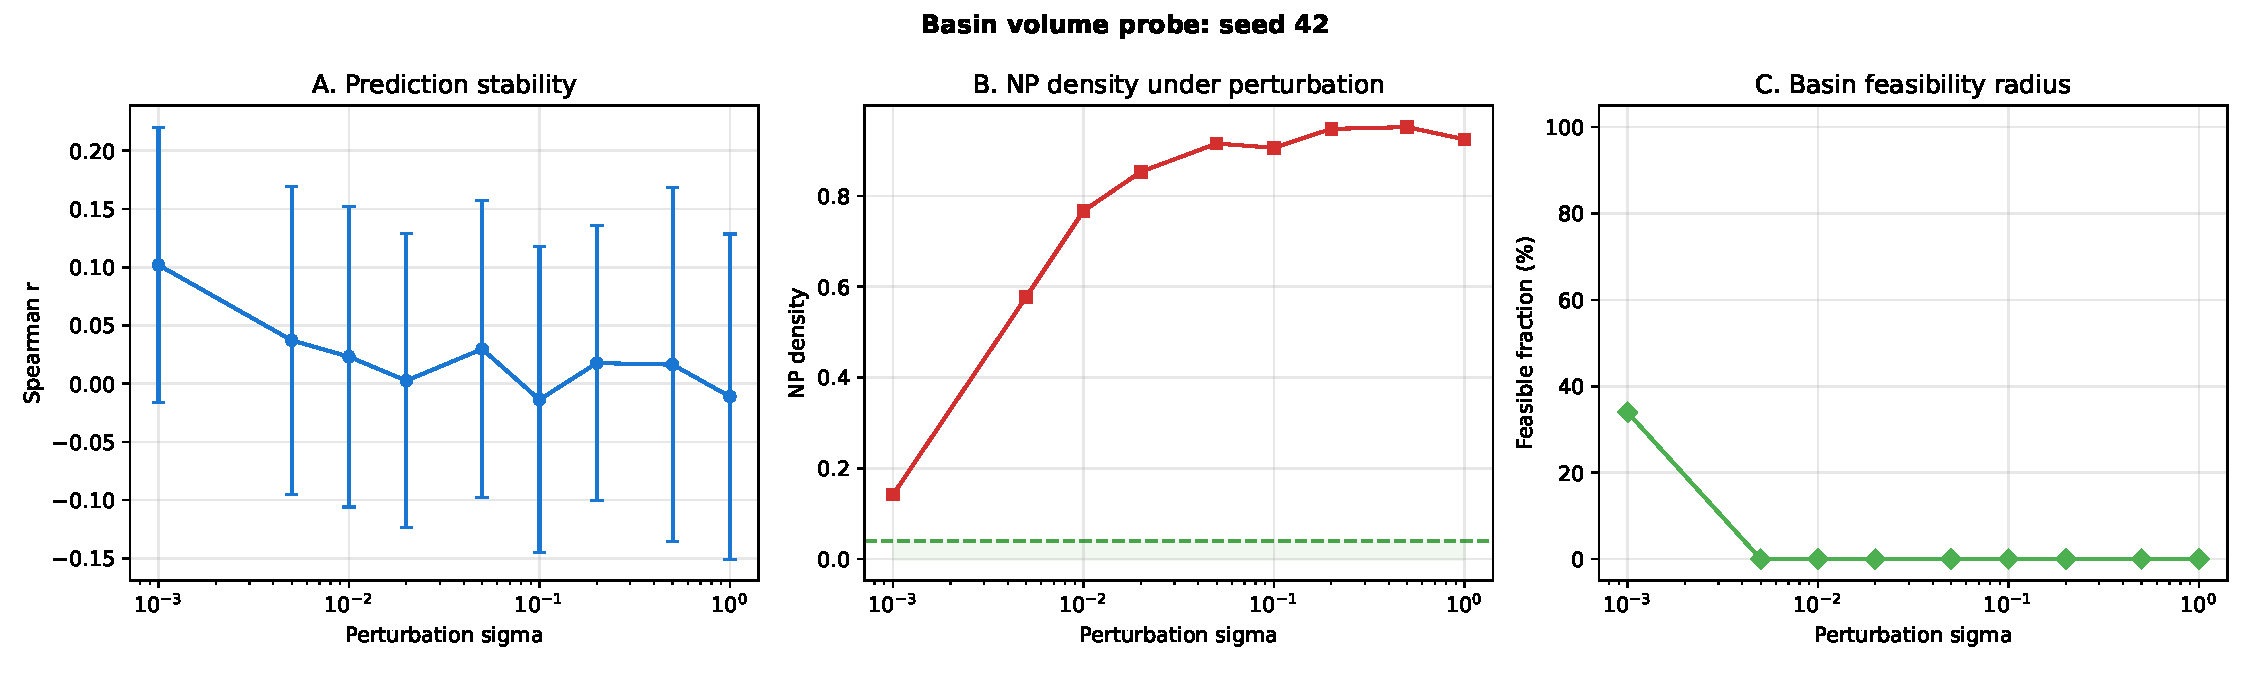
\includegraphics[width=\textwidth]{../figures/basin_volume_seed_42.pdf}
\caption{Type A (seed 42): catastrophic collapse at $\sigma = 0.001$.}
\end{subfigure}

\vspace{0.8em}

\begin{subfigure}[t]{\textwidth}
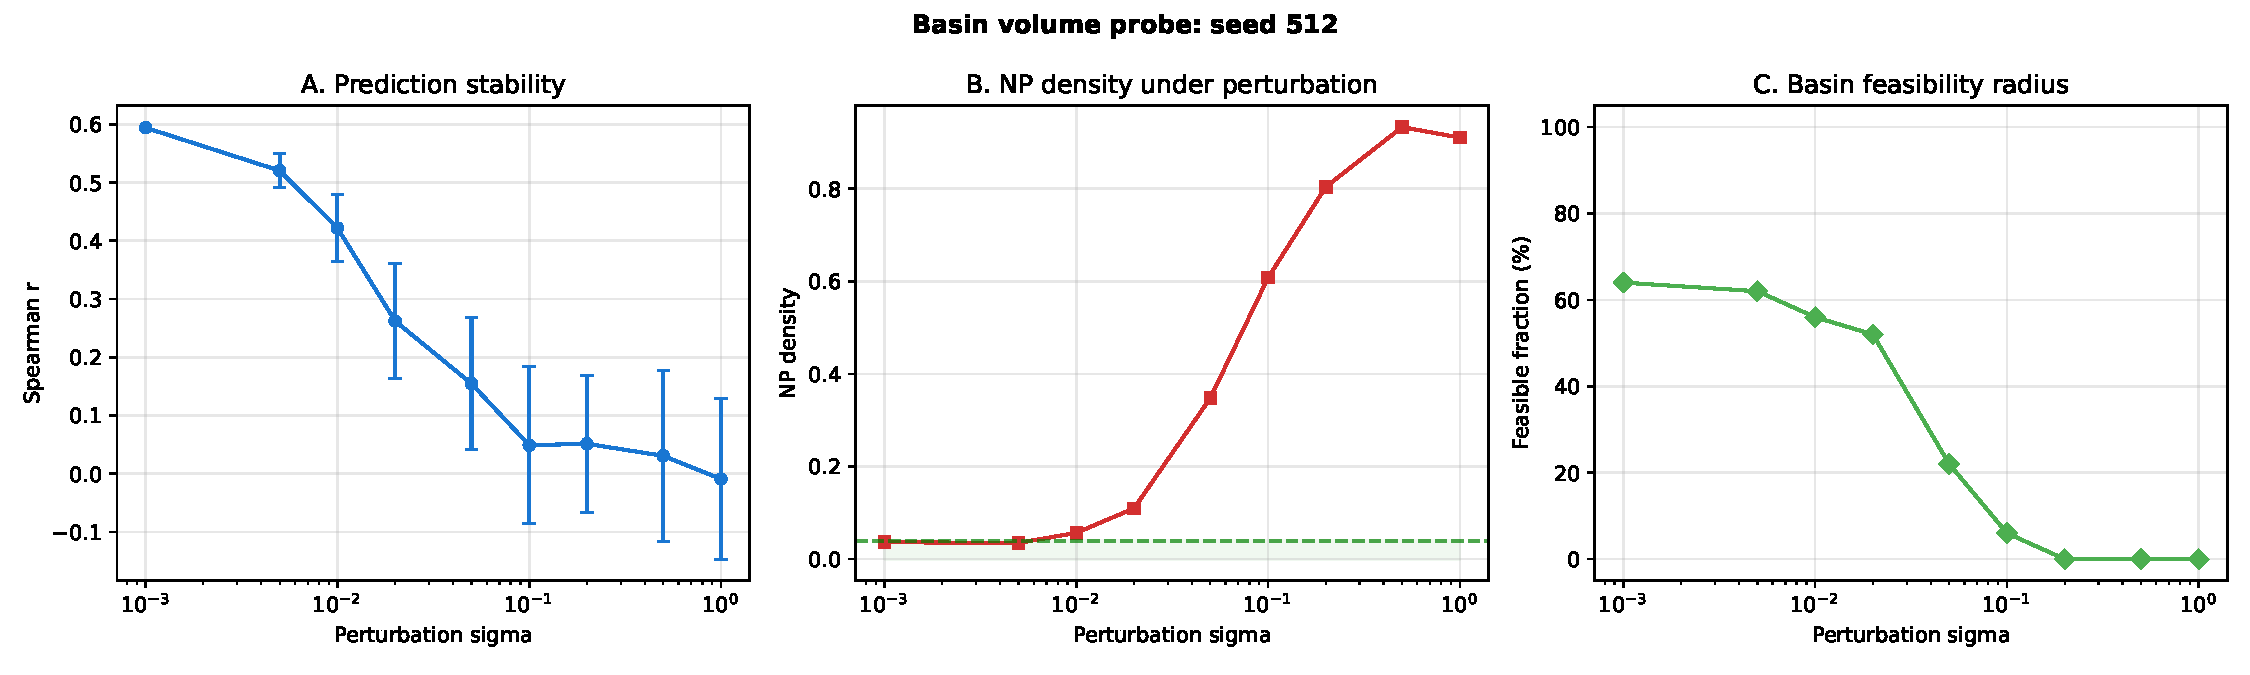
\includegraphics[width=\textwidth]{../figures/basin_volume_seed_512.pdf}
\caption{Type C (seed 512): graceful degradation.}
\end{subfigure}
\caption{Perturbation robustness comparison. Each point: mean over 50
Gaussian perturbations. Type A's precision-tuned compliance structure
collapses under minimal noise; Type C's signal-only compliance degrades
smoothly.}
\label{fig:perturbation}
\end{figure}

Type~A is catastrophically fragile: $\sigma = 0.001$ per coordinate (0.015\% of the genome's
L2 norm $\|\btheta\|_2 \approx 6.7$) collapses $\rho$ from 0.5942 to 0.102. Type~C degrades gracefully, retaining
mean $\rho = 0.594$ and 64\% feasibility at the same noise level.

%% ============================================================
\section{Covariance-Induced Drift}
\label{sec:drift}
%% ============================================================

\subsection{Within-Seed Drift Trajectory}

Per-generation tracking of seed~42 (8000 generations, diagnostics every 10
generations) reveals drift through five phases (Figure~\ref{fig:dynamics}):

\begin{enumerate}
\item \textbf{Signal acquisition} (gen 0--300). Rapid $\rho$ improvement
  ($0.50 \to 0.57$). Sensitivity importance: 3--9\% (noisy).

\item \textbf{L2 compression} (gen 300--2700). L2 regularization compresses
  sensitivity parameters. Sensitivity importance drops to 0.3\%. This is the
  Type~C regime.

\item \textbf{Post-restart drift onset} (gen 3970--6100). Generations
  2700--3970 are a stagnation interval during which $\sigma$ collapses
  below $10^{-6}$, triggering restart. After restart, sensitivity importance
  begins growing.
  First punctuated jump: 3\% $\to$ 13\% at gen~4940.

\item \textbf{Sensitivity-dominated regime} (gen 6200--7600).
  Two further jumps (18\%$\to$51\% at gen 6200--6500, and 52\%$\to$76\% at gen
  7000--7400) drive sensitivity to its peak. During this phase, $\rho$ changes by
  only $+0.0025$ while sensitivity importance increases by $\sim$58 percentage
  points (18\% to 76\% peak).

\item \textbf{Lock-in} (gen 7600+). Genome stabilizes at $\rho = 0.5942$,
  sensitivity = 69.8\% (settling from the 76\% transient peak). Further restart produces no change.
\end{enumerate}

\begin{figure}[t]
\centering
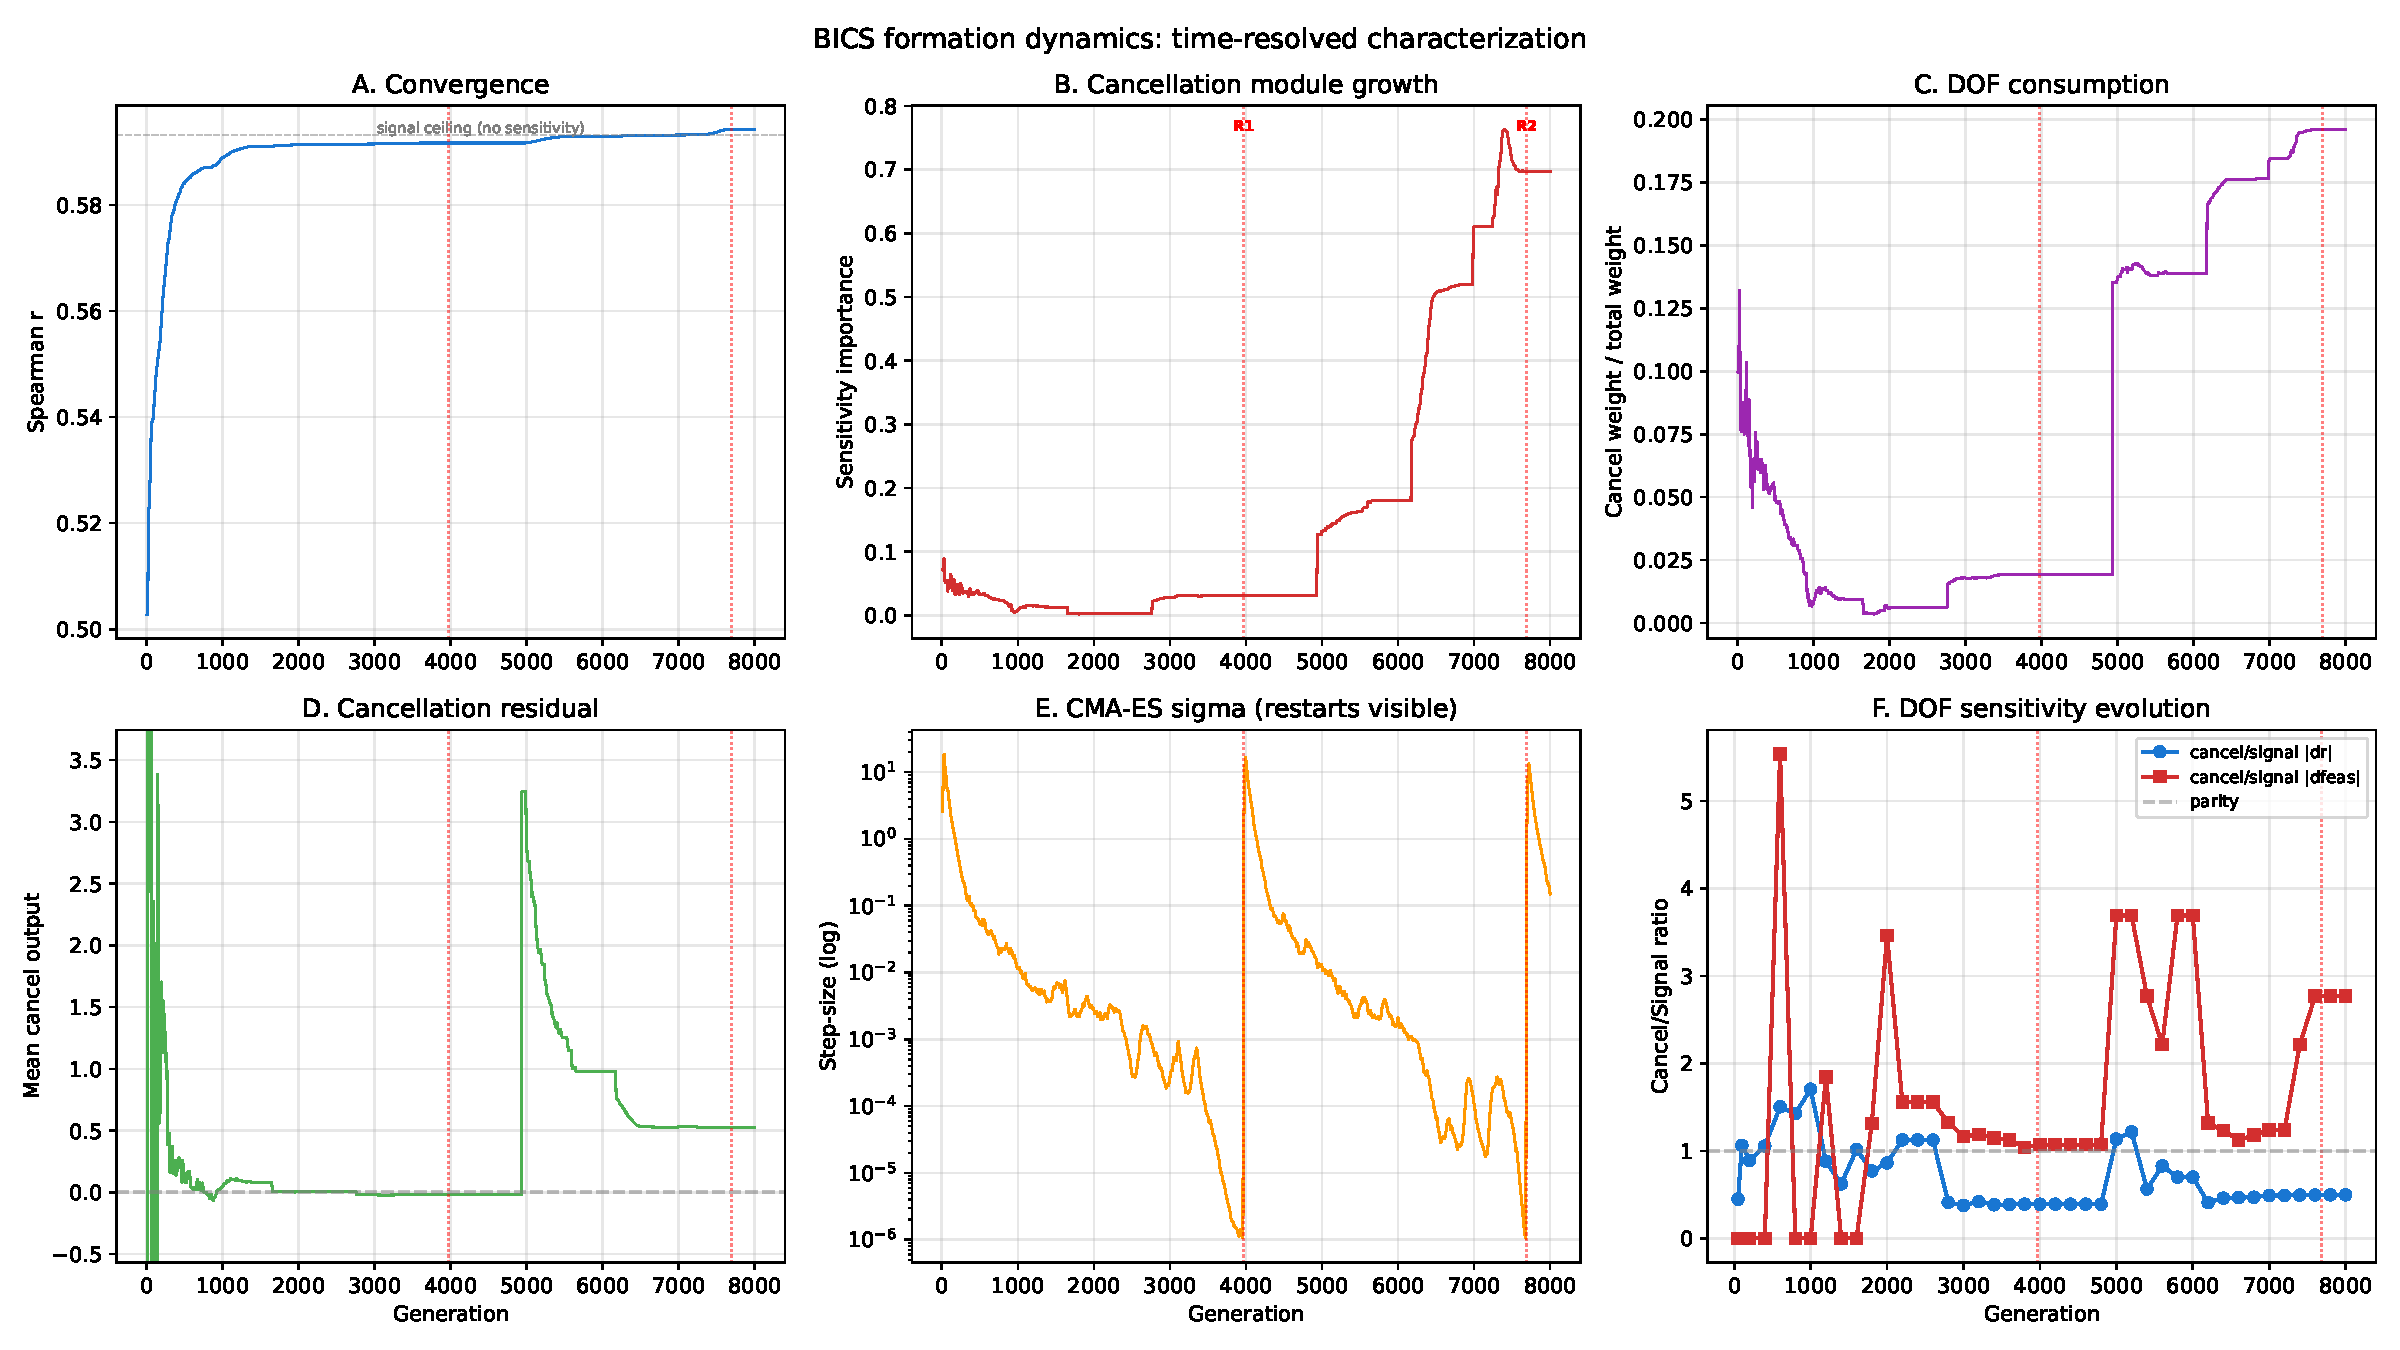
\includegraphics[width=\textwidth]{../figures/bics_dynamics.pdf}
\caption{Drift dynamics for seed~42 (8000 generations), six panels in 3$\times$2
layout. (a)~Spearman $\rho$ with signal ceiling (dashed, from sensitivity-ablated
genome). (b)~Sensitivity importance $\phi_{\text{sens}}$ growing through three
punctuated jumps; R1, R2 mark restart events. (c)~Degrees of freedom (DOF: number of genome dimensions with $>$1\%
of total variance) consumed by compliance subspace. (d)~Compliance residual
trajectory. (e)~Sigma trajectory (log scale). (f)~DOF responsiveness
(feasibility change per unit DOF change). The decoupling is clear:
$\rho$ changes by $+$0.003 (${\sim}$0.5\%) over generations 2000--7600 while $\phi_{\text{sens}}$
increases 230$\times$.}
\label{fig:dynamics}
\end{figure}

Seed~137 shows qualitatively similar dynamics but with different timing:
$\rho$ plateau at gen~4000 (vs.\ gen~2000 for seed~42), sensitivity $\geq$10\%
at gen~7400 (vs.\ gen~4940). The jumps are state-controlled (triggered by
exhaustion of signal-only improvement), not generation-controlled.

\subsection{Short Runs vs.\ Long Runs}

The drift hypothesis predicts that short runs should find Type~C (before
covariance learns sensitivity--signal couplings) while long runs should drift
to Type~B. We tested this with 5 independent seeds (2000--2004) run for
2000 generations under standard full CMA-ES:

\begin{table}[t]
\caption{Regime distribution by search duration. The 2000-gen seeds
(2000--2004) are independent from the 8000-gen seeds (42, 137, 256, 512, 1024).
This is a between-subjects comparison; within-seed evidence comes from the
trajectory analysis (Figure~\ref{fig:dynamics}), where seed~42 is Type~C at
gen~2000 and Type~A at gen~8000.}
\label{tab:duration}
\centering
\begin{tabular}{lccc}
\toprule
Duration & Type A & Type B & Type C \\
\midrule
2000 generations (seeds 2000--2004) & 0 & 1 (20\%) & \textbf{4 (80\%)} \\
8000 generations (seeds 42, 137, 256, 512, 1024) & 1 (20\%) & \textbf{3 (60\%)} & 1 (20\%) \\
\bottomrule
\end{tabular}
\end{table}

The regime distribution inverts: 80\% Type~C at 2000 generations versus 20\%
at 8000 generations. While these are different seed sets (Table~\ref{tab:duration}),
the within-seed trajectory data provides direct confirmation: seed~42's
per-generation diagnostics show $\phi_{\text{sens}} < 0.05$ (Type~C) at gen~2000
and $\phi_{\text{sens}} = 0.698$ (Type~A) at gen~8000.

\subsection{Irreversibility}
\label{sec:irreversibility}

We tested whether Type~B endpoints can return to Type~C under extended
search. Using 5 Type~B endpoints from the 30-seed cross-optimizer experiment
(seeds with $\phi_{\text{sens}} > 0.05$), we ran 3000-generation escape
attempts under four conditions (Table~\ref{tab:interventions}).

\begin{table}[t]
\caption{Extended escape attempts from Type B endpoints (3000 generations,
5 seeds per condition). ``Returned to C'': final $\phi_{\text{sens}} \leq 0.05$.
The asymmetry between full CMA-ES (1/10 return) and sep-CMA-ES (5/5) or
frozen covariance (4/5) confirms that learned covariance structure, not
the landscape alone, maintains the lock.}
\label{tab:interventions}
\centering
\begin{tabular}{llc}
\toprule
Condition & Description & Returned to C \\
\midrule
Full CMA-ES (standard) & Full $\bC$, $\sigma_0 = 0.3$ & 0/5 \\
Full CMA-ES (large $\sigma$) & Full $\bC$, $\sigma_0 = 1.0$ & 1/5 \\
sep-CMA-ES from B & Diagonal $\bC$, initialized at Type~B & \textbf{5/5} \\
Frozen covariance & $\bC = \bI$ forced & \textbf{4/5} \\
\bottomrule
\end{tabular}
\end{table}

Full CMA-ES returns to Type~C in only 1/10 combined trials (standard + large
$\sigma$). In contrast, sep-CMA-ES achieves 5/5 returns and frozen covariance
4/5. This asymmetry rules out a pure landscape-lock explanation: the
\emph{same} starting points are escapable when cross-dimensional adaptation
is removed. The lock requires the ongoing covariance learning that
re-discovers sensitivity--signal couplings even after perturbation.

\textbf{Causal interpretation.} Discovery of the deceptive attractor requires
full covariance (Section~\ref{sec:crossopt}), and \emph{maintenance} of the
lock also requires it. sep-CMA-ES, starting from the same Type~B genome,
cannot sustain the sensitivity--signal covariance structure and drifts back
to Type~C under L2 regularization pressure.

%% ============================================================
\section{Cross-Optimizer Comparison}
\label{sec:crossopt}
%% ============================================================

If the drift were a property of the fitness landscape alone, all optimizer
variants should exhibit it given sufficient time. We ran all three CMA-ES
variants for 3000 generations on 30 independent seeds (seeds 1--30),
using population size $\lambda = 50$ and checkpoints at generations
500, 1000, 2000, and 3000.

\begin{table}[t]
\caption{Cross-optimizer comparison (30 seeds, 3000 generations).
Drift rate: fraction of seeds reaching $\phi_{\text{sens}} > 0.05$ (Type~B/A).
Fisher's exact test (one-sided) and Mann-Whitney $U$ test compare
$\phi_{\text{sens}}$ distributions.}
\label{tab:crossopt}
\centering
\begin{tabular}{lcccc}
\toprule
Optimizer & Drift rate & Mean $\phi_{\text{sens}}$ & vs.\ Full (Fisher) & vs.\ Full (MW) \\
\midrule
Full CMA-ES & \textbf{22/30 (73\%)} & 0.103 & --- & --- \\
sep-CMA-ES & 13/30 (43\%) & 0.048 & $p = 0.018$ & $p = 0.001$ \\
Isotropic ES & 5/30 (16\%) & 0.038 & $p < 0.001$ & --- \\
\bottomrule
\end{tabular}
\end{table}

\textbf{Three-tier drift gradient} (Table~\ref{tab:crossopt}).
Full CMA-ES: 73\% drift rate with mean $\phi_{\text{sens}} = 0.103$.
sep-CMA-ES: 43\% drift rate ($p = 0.018$, Fisher one-sided; $p = 0.001$,
Mann-Whitney $U = 659$). Isotropic ES: 16\% drift rate ($p < 0.001$).
The ordering (full $\gg$ sep $>$ isotropic) is statistically
significant and consistent with the 3-seed pilot study.

\textbf{Scale of the effect.} The 30-percentage-point gap between full and
sep-CMA-ES (73\% vs.\ 43\%) is modest in absolute terms but significant
in the $\phi_{\text{sens}}$ magnitude: full CMA-ES mean $\phi_{\text{sens}}$
is $2.1\times$ that of sep-CMA-ES. The drift is more frequent and more severe under full covariance.

\textbf{Convergence speed caveat.} The three variants may differ in effective
convergence speed. In the 5-seed pilot study (Table~\ref{tab:types}),
full CMA-ES achieves $\rho \approx 0.597$ versus sep-CMA-ES
$\rho \approx 0.591$; in the 30-seed experiment the gap narrows
($\Delta\rho \approx 0.003$), suggesting sep-CMA-ES has not fully
converged but the performance cost is modest. We cannot
rule out that sep-CMA-ES at substantially longer durations (e.g., 50{,}000
generations) might eventually drift. However, the population scaling experiments
(Section~\ref{sec:lambda}) show that increasing $\lambda$ \emph{widens} the
gap rather than closing it, arguing against a convergence-speed explanation.

%% ============================================================
\section{The Mechanism Chain}
\label{sec:mechanism}
%% ============================================================

\subsection{Signal--Compliance Decomposition}

Ablation analysis on the Type~A genome (seed~42) identifies two functional modules:

\begin{itemize}
\item \textbf{Signal axis}: spectral entropy (primary), algebraic degree,
  nonlinearity, autocorrelation sum. Ablation impact: spectral entropy removal
  drops $\rho$ by 0.425 (72\% loss); algebraic degree by 0.222 (37\%).

\item \textbf{Compliance axis}: sensitivity self-quadratic ($q_{7,7} = -0.066$)
  and threshold gating ($a_7 = +0.355$). Contribute $\Delta\rho = 0.001$ to
  prediction but reduce natural proof density from 1.000 to 0.0186, a
  54$\times$ reduction essential for feasibility.
\end{itemize}

The compliance module exhibits three diagnostic properties: \emph{precision
fragility} ($\sigma = 0.01$ noise on 10 quadratic weights destroys 92\% of
$\rho$), \emph{sign coherence} (flipping linear or quadratic alone:
$-$72\%/$-$29\%; flipping both: $-$0.6\%), and \emph{non-substitutability}
(all 9 feature substitutions yield $\rho \in [0.08, 0.22]$).

\subsection{Causal Pathway}

The drift has two stages:

\textbf{Discovery (covariance-driven).} Full CMA-ES covariance $\bC$ learns
that sensitivity--signal coupled perturbations produce rank improvements. These
improvements are genuine but small ($\Delta\rho < 0.005$). Rank-one and
rank-$\mu$ updates amplify sampling along these coupled directions, creating a
positive feedback loop. sep-CMA-ES cannot execute this step because diagonal
adaptation cannot learn cross-dimensional correlations.

\textbf{Lock (covariance-reinforced).} Once sensitivity dimensions accumulate
sufficient mass, the adapted covariance structure amplifies sampling along
sensitivity--signal directions, reinforcing the attractor. The escape
experiments (Table~\ref{tab:interventions}) confirm that this lock requires
ongoing covariance learning: freezing $\bC = \bI$ enables escape in 4/5
trials, while full CMA-ES escapes in only 1/10.

Covariance adaptation drives the genome into the deceptive attractor
and holds it there; removing covariance learning allows escape
(Section~\ref{sec:irreversibility}).

%% ============================================================
\section{Structural Irreducibility}
\label{sec:irreducibility}
%% ============================================================

\begin{conjecture}[Structural Irreducibility of Covariance-Induced Drift]
\label{conj:irreducibility}
The irreversible drift from Type~C to Type~B or Type~A under full CMA-ES
requires the simultaneous presence of three structural conditions:
\begin{enumerate}
\item[\emph{(C1)}] \emph{Non-smooth objective}: the fitness function is
  rank-based, creating piecewise-constant regions where gradient information
  is available only at rank-swap boundaries.
\item[\emph{(C2)}] \emph{Cross-dimensional interactions}: the parameter space
  contains quadratic cross-terms that the covariance matrix can learn as
  coupled perturbation directions.
\item[\emph{(C3)}] \emph{Discontinuous constraint boundaries}: barrier
  constraints are binary with sharp feasibility boundaries, creating
  disconnected feasible basins.
\end{enumerate}
Removing any single condition eliminates the drift phenomenon.
\end{conjecture}

We test each condition by same-problem ablation on the Boolean complexity
domain (30 seeds per condition, 3000 generations, $\lambda = 50$).

\textbf{C2: Cross-dimensional interactions (primary driver).}
The cross-optimizer comparison (Section~\ref{sec:crossopt}) directly ablates
C2: sep-CMA-ES restricts covariance to a diagonal matrix, reducing drift
from 73\% to 43\% (Fisher $p = 0.018$). This differential persists even
when C1 is removed (see below), establishing C2 as the primary necessary
condition.

\textbf{C1: Non-smooth objective (amplifier, not necessary).}
Replacing Spearman correlation with MSE on the same problem preserves the
full$>$sep differential: full CMA-ES drifts in 43\% of runs versus 3\% for
sep-CMA-ES (Fisher $p = 0.0002$). The non-smooth objective amplifies drift
(73\% with Spearman vs.\ 43\% with MSE for full CMA-ES) but is not necessary
for it. C1's role is to create piecewise-constant regions where the covariance
can learn sensitivity--signal couplings without gradient domination; MSE
provides gradient signals that partially suppress but do not eliminate
covariance-driven exploration.

\textbf{C3: Discontinuous constraints (amplifier, not necessary).}
Replacing binary barrier constraints with soft quadratic penalties reduces
but does not eliminate the full$>$sep gap: full drifts in 66\% versus sep 40\%
(Fisher $p = 0.035$). Isotropic drift also rises to 40\% under soft
penalties (vs.\ 16\% with binary), suggesting that binary constraints
selectively suppress drift in restricted-covariance variants more than in
full CMA-ES. C3 amplifies the differential but is not strictly necessary.

\textbf{Summary.} The original conjecture, that all three
conditions are jointly necessary, is partially supported. C2 is
necessary (ablation eliminates the differential). C1 and C3 are amplifiers:
each increases drift rates and widens the full$>$sep gap, but neither is
individually necessary. The strongest drift occurs when all three conditions
co-occur (73\% full vs.\ 16\% isotropic), consistent with a reinforcing
interaction rather than strict necessity of each condition.

\subsection{Comparison with Simplified Models}

The same-problem ablations above test each condition on the Boolean complexity
domain. As a complementary test, we constructed three simplified synthetic
models that individually relax conditions:

\begin{enumerate}
\item \emph{Latent factor model} (relaxes C1 \& C3: smooth signal, linear
  constraint on sensitivity-weighted output). Full CMA-ES converged immediately
  with no drift opportunity. All variants found identical solutions.

\item \emph{Rank-disruption model} (preserves C1, partially relaxes C2:
  rank-based fitness, correlated signal columns). Isotropic outperformed full
  CMA-ES on drift (opposite pattern), because correlated signals prevented
  sep-CMA-ES convergence.

\item \emph{Rotated ellipsoid with barrier} (relaxes C1: smooth quadratic
  objective, binary constraint on sensitivity dimensions). All three variants
  found the same penalty-weighted optimum with identical drift rates.
\end{enumerate}

None reproduced the differential drift pattern (full $\gg$ sep $>$ iso),
consistent with the same-problem ablation results. The simplified models
additionally confirm that the conditions interact: relaxing any
single condition in isolation is insufficient to create the pattern, but
the C1 and C3 same-problem ablations show the pattern \emph{persists} (at
reduced magnitude) even when one amplifying condition is removed.

%% ============================================================
\section{Population Scaling}
\label{sec:lambda}
%% ============================================================

If the drift mechanism operates through covariance learning, larger populations
(which provide more samples for covariance estimation) should amplify the
effect. We tested four population sizes $\lambda \in \{17, 50, 100, 200\}$
with 10 seeds each, comparing full CMA-ES against sep-CMA-ES
(Table~\ref{tab:lambda}).

\begin{table}[t]
\caption{Drift rate by population size ($\lambda$). 10 seeds per cell,
3000 generations. $\lambda = 17$ is the CMA-ES default for $p = 85$;
$\lambda = 50$ is used in all other experiments. The monotonic non-decreasing trend in
full$-$sep gap with $\lambda$ is consistent with improved covariance
estimation enabling stronger cross-dimensional learning.}
\label{tab:lambda}
\centering
\begin{tabular}{lcccc}
\toprule
$\lambda$ & Full drift & Sep drift & Gap (pp) & Fisher $p$ \\
\midrule
17  & 9/10 (90\%)  & 6/10 (60\%)  & 30  & 0.30 \\
50  & 8/10 (80\%)  & 5/10 (50\%)  & 30  & 0.35 \\
100 & 9/10 (90\%)  & 1/10 (10\%)  & 80  & 0.001 \\
200 & \textbf{10/10 (100\%)} & \textbf{0/10 (0\%)} & \textbf{100} & $< 0.001$ \\
\bottomrule
\end{tabular}
\end{table}

The drift gap is monotonically non-decreasing, from 30 percentage points at
$\lambda = 17$ to complete separation at $\lambda = 200$. At $\lambda = 200$,
full CMA-ES drifts in every run while sep-CMA-ES drifts in none.

\textbf{Mechanism.} Larger $\lambda$ improves covariance
estimation quality~\citep{hansen2003reducing}, enabling more accurate
learning of sensitivity--signal cross-dimensional couplings. The monotonically non-decreasing trend
in drift differential directly supports the covariance-learning
mechanism: if drift were caused by some other property of full CMA-ES
(e.g., mean update differences), the gap would not systematically widen
with improved covariance estimation.

\textbf{Practical implication.} Practitioners commonly increase $\lambda$
for high-dimensional problems to improve convergence reliability. Our results
show that this standard practice \emph{exacerbates} covariance-induced drift
under barrier constraints. The recommended diagnostic (comparing full vs.\
sep-CMA-ES) becomes more important as $\lambda$ grows.

%% ============================================================
\section{Adaptive Mitigation}
\label{sec:mitigation}
%% ============================================================

We tested whether the drift can be prevented by monitoring
$\phi_{\text{sens}}$ and switching from full to sep-CMA-ES when drift is
detected. We implemented an adaptive strategy: run full CMA-ES, but switch
to sep-CMA-ES whenever $\phi_{\text{sens}} > 0.05$ at a checkpoint, and
switch back when $\phi_{\text{sens}} \leq 0.05$. We tested this on 30 seeds
(3000 generations, $\lambda = 50$).

The adaptive strategy achieves a drift rate of 70\% (21/30), comparable to
pure full CMA-ES (73\%) and with mean $\rho = 0.583$ (vs.\ 0.584 for full).
The mean number of full$\to$sep switches per run is 0.6, indicating that the
intervention fires too late: by the time $\phi_{\text{sens}}$ crosses the
threshold, the genome has already entered a region where even sep-CMA-ES
cannot reverse the drift within the remaining budget.

This negative result is consistent with the irreversibility finding
(Section~\ref{sec:irreversibility}): the Type~B attractor, once entered,
traps the optimizer regardless of subsequent covariance restriction. Effective
mitigation would require either (i)~preemptive switching before
$\phi_{\text{sens}}$ crosses the threshold, or (ii)~using sep-CMA-ES
exclusively when binary constraints are present, accepting the modest
performance cost ($\Delta\rho \approx 0.003$).

%% ============================================================
\section{Discussion}
\label{sec:discussion}
%% ============================================================

\subsection{Implications for Constrained CMA-ES}

Existing constraint-handling mechanisms for CMA-ES~\citep{arnold2012cmaes,
kramer2010cmaes,atamna2016augmented} primarily address continuous constraints
with smooth boundaries. Our findings identify a different failure
mode under binary constraints with non-smooth objectives. The covariance matrix
learns cross-dimensional couplings that are locally beneficial for the
unconstrained objective but cross constraint boundaries. This is distinct
from the step-size difficulties documented for smooth constraints, where the
optimizer ``bounces'' off boundaries. Here, the optimizer \emph{crosses} the
boundary and finds a locally superior infeasible region from which it cannot
return.

For practitioners, our results suggest concrete strategies:
\begin{enumerate}
\item \textbf{Default to sep-CMA-ES} under binary constraints. The performance
  cost is modest ($\Delta\rho \approx 0.003$) and the feasibility improvement is
  large (Section~\ref{sec:mitigation}).
\item \textbf{If full CMA-ES is required}, monitor $\phi_{\text{sens}}$ (or
  analogous overhead metrics). If parameter dimensions with negligible objective
  contribution accumulate mass, this signals compliance drift.
\item \textbf{Avoid large $\lambda$} when binary constraints are present.
  The population scaling results (Section~\ref{sec:lambda}) show that larger
  populations exacerbate drift rather than mitigating it.
\item \textbf{Reactive switching is insufficient.} Switching from full to
  sep-CMA-ES after drift detection does not reverse the damage
  (Section~\ref{sec:mitigation}); preemptive variant selection is required.
\end{enumerate}

\subsection{Structural Overhead of Barrier Compliance}

The signal--compliance decomposition shows that barrier constraints impose
a structural tax on representation capacity. In the Type~A solution, 70\% of
genome parameters serve a precision-tuned compliance function contributing
$\Delta\rho = 0.001$. This tax is not inevitable (Type~C achieves compliance
with zero overhead) but is the most common long-run outcome under full CMA-ES.

\subsection{Limitations}

\textbf{Single domain.} All findings are established on the Boolean complexity
domain. While the controlled ablations (Section~\ref{sec:irreducibility}) and
population scaling (Section~\ref{sec:lambda}) test the mechanism in isolation,
replication on other constrained optimization problems with binary constraints
would strengthen the external validity.

\textbf{Generation budget.} All 30-seed experiments use 3000 generations
(vs.\ 8000 in the pilot study). While checkpoints show drift stabilizes by
generation 2000 in most runs, we cannot rule out that longer durations would
change the relative rankings.

\textbf{Barrier proxy fidelity.} The barrier implementations are heuristic
proxies, not exact complexity-theoretic conditions. The qualitative landscape
structure is expected to persist under threshold variation, but this has not
been systematically tested.

%% ============================================================
\section{Conclusion}
\label{sec:conclusion}
%% ============================================================

We have documented \emph{covariance-induced irreversible drift}: a failure mode
where full CMA-ES systematically transitions from feasible, low-overhead
solutions to infeasible, high-overhead ones through cross-dimensional
covariance adaptation. In a 30-seed controlled study, full CMA-ES drifts in
73\% of runs versus 43\% for sep-CMA-ES and 16\% for isotropic ES (Fisher
$p = 0.018$). The drift is genuinely irreversible under full covariance
(1/10 escape) but readily reversible under sep-CMA-ES (5/5 escape) or
frozen covariance (4/5), establishing that learned covariance structure
maintains the lock.

Controlled ablations show that cross-dimensional adaptation (C2) is the
primary necessary condition ($p = 0.0002$), while the non-smooth objective
(C1) and binary constraints (C3) act as amplifiers. Population scaling
experiments show monotonically non-decreasing drift separation, reaching complete
separation (100\% full vs.\ 0\% sep) at $\lambda = 200$, providing direct
mechanistic confirmation through improved covariance estimation quality.

Adaptive mitigation (switching to sep-CMA-ES upon drift detection) fails
because intervention arrives too late: the Type~B attractor traps the
optimizer before monitoring can respond. For
barrier-constrained problems with the structural properties identified here,
sep-CMA-ES should be the default variant, accepting the modest performance
cost ($\Delta\rho \approx 0.003$) to guarantee feasibility.

The open question is external validity: does the phenomenon
arise on other constrained optimization problems with C1--C3 structure?
The population scaling result suggests it may occur in any setting
where cross-dimensional covariance learning can discover constraint-violating
directions that yield marginal objective improvement.

\paragraph{Reproducibility.}
All experimental code, data files (per-generation diagnostics, genome
checkpoints, interpolation results), and analysis scripts are available at
\url{[anonymized repository]}.

\vskip 0.2in
\bibliography{references}

\appendix

%% ============================================================
\section{Complete Experimental Timeline}
\label{app:timeline}
%% ============================================================

\begin{table}[t]
\caption{Experimental phases and key findings. Phases 1--3 used a buggy ordinal
ranking implementation (fixed in Phase~4); all quantitative results in the paper
use the corrected implementation.}
\label{tab:timeline}
\centering
\small
\begin{tabular}{clp{7cm}}
\toprule
Phase & Focus & Key Finding \\
\midrule
1--3 & Setup, search, analysis & Initial infrastructure and runs (pre-fix) \\
4 & Tie-handling fix & Train/test gap was ordinal ranking artifact \\
5 & Mechanism decomposition & Signal + compliance decomposition \\
6 & Robustness validation & NP barrier is the only binding constraint \\
7 & Attack experiments & Precision sensitivity, sign coherence \\
8 & Curvature hypothesis & Refuted: sensitivity is compliance, not correction \\
9 & Compliance subspace & Compliance subspace defined and quantified \\
10 & Formation dynamics & Punctuated equilibrium: 3 discrete jumps \\
11 & Mechanism decomposition & NP compliance, path-dependent allocation \\
12 & Path dependence & Two different compliance strategies \\
13 & Basin disconnection & $\rho$ goes negative between basins \\
14 & Basin topology & Three solution types across 5 seeds \\
15 & Type C analysis & Type C superior on all axes \\
16 & Reachability & 80\% Type C at 2000 gen; 60\% B + 20\% A at 8000 gen \\
17 & Covariance dissection & Lock is landscape-level \\
18 & Cross-optimizer (pilot) & Full: 3/3; sep: 0/3; isotropic: 1/3 drift \\
19 & 30-seed cross-optimizer & Full 73\%, sep 43\%, iso 16\%; $p = 0.018$ \\
20 & C1 ablation (MSE) & Full 43\% vs sep 3\%; $p = 0.0002$ \\
21 & C3 ablation (soft) & Full 66\% vs sep 40\%; $p = 0.035$ \\
22 & Lambda scaling & 100\% vs 0\% separation at $\lambda = 200$ \\
23 & Extended escape & Full 1/10 vs sep 5/5 return \\
24 & Adaptive mitigation & 70\% drift; reactive switching insufficient \\
\bottomrule
\end{tabular}
\end{table}

%% ============================================================
\section{Genome Representation Details}
\label{app:genome}
%% ============================================================

The 85-dimensional genome $\btheta = (\mathbf{w}, \mathbf{q}, \mathbf{a}, \mathbf{t})$:

\begin{itemize}
\item $\mathbf{w} \in \R^{10}$: linear weights on each feature.
\item $\mathbf{q} \in \R^{55}$: upper-triangular quadratic weights on
  $m_i(f) \cdot m_j(f)$ for $i \leq j$ (10 self-quadratic + 45 cross-terms).
\item $\mathbf{a} \in \R^{10}$: activation coefficients for threshold gating.
\item $\mathbf{t} \in \R^{10}$: threshold parameters.
\end{itemize}

Sensitivity (alphabetical position 7; storage index 8 in the code repository)
participates in 13 ``compliance'' dimensions: 1 linear weight ($w_7$),
10 quadratic terms ($q_{i,7}$ for $i = 0, \ldots, 9$), 1 activation ($a_7$),
1 threshold ($t_7$), where subscripts follow the alphabetical convention.
The remaining
72 dimensions are ``signal'' dimensions.

This partition is defined a priori by feature identity, validated by
finite-difference gradient analysis: compliance dimensions have $2.77\times$
higher feasibility responsiveness and $0.50\times$ lower correlation
responsiveness than signal dimensions.

%% ============================================================
\section{Full Interpolation Results}
\label{app:interpolation}
%% ============================================================

\begin{table}[t]
\caption{Complete pairwise interpolation between all five seed endpoints (21
interpolants per pair).}
\label{tab:interpolation_full}
\centering
\begin{tabular}{llrrr}
\toprule
Path & Types & min $\rho$ & max density & feas.\ pts \\
\midrule
42--256 & A--B & +0.27 & 0.076 & 8/21 \\
137--1024 & B--B & +0.33 & 0.396 & 1/21 \\
42--1024 & A--B & +0.10 & 0.398 & 2/21 \\
137--256 & B--B & +0.20 & 0.541 & 0/21 \\
256--1024 & B--B & $-$0.02 & 0.961 & 1/21 \\
42--137 & A--B & $-$0.07 & 0.856 & 1/21 \\
256--512 & B--C & +0.18 & 0.958 & 1/21 \\
512--1024 & C--B & +0.18 & 0.993 & 2/21 \\
42--512 & A--C & $-$0.14 & 0.996 & 2/21 \\
137--512 & B--C & $-$0.16 & 1.000 & 1/21 \\
\bottomrule
\end{tabular}
\end{table}

\begin{figure}[t]
\centering
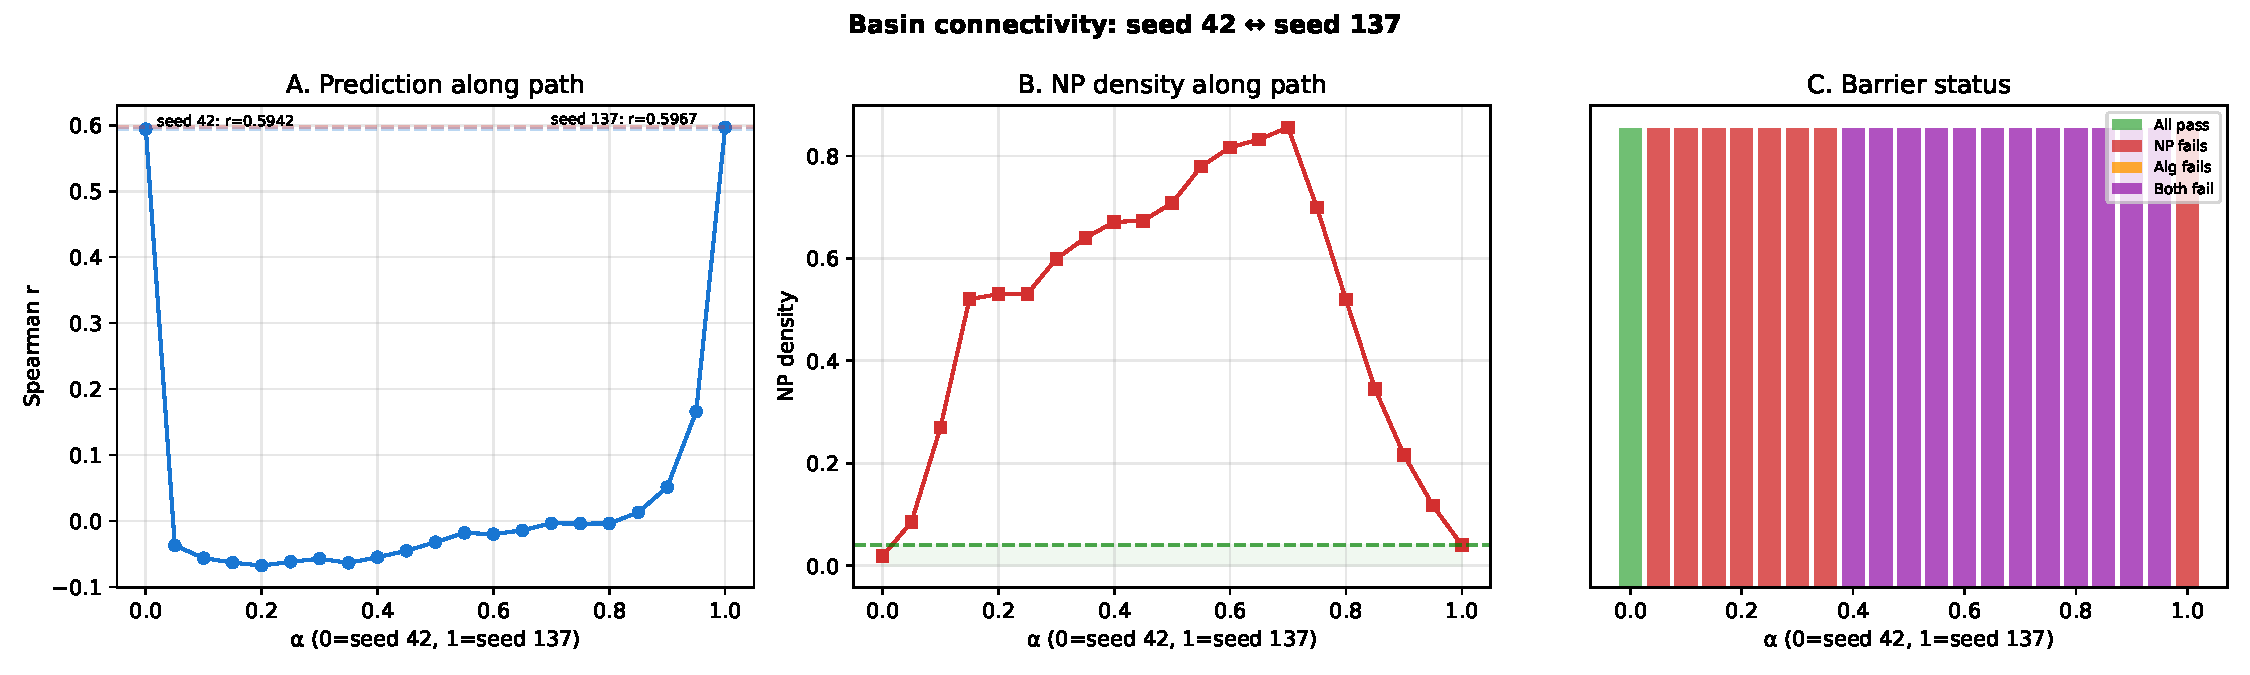
\includegraphics[width=0.9\textwidth]{../figures/interpolation_42_137.pdf}
\caption{Interpolation between Type~A (seed 42, $\alpha=0$) and Type~B
(seed 137, $\alpha=1$). $\rho$ drops to $-0.07$ at $\alpha = 0.2$; NP density
peaks at 0.856; the intermediate region violates two barriers simultaneously.}
\label{fig:interpolation}
\end{figure}

%% ============================================================
\section{Local Continuation Analysis}
\label{app:continuation}
%% ============================================================

To confirm Type~C is a genuine basin (not a zero-measure spike), we perturbed
seed~512's genome with Gaussian noise and applied 100-generation CMA-ES
refinement (Table~\ref{tab:continuation}).

\begin{table}[t]
\caption{Local continuation from perturbed Type~C genome. 10 perturbations
per $\sigma$, 100-generation refinement. Recovery: $\rho > 0.55$ and feasible.}
\label{tab:continuation}
\centering
\begin{tabular}{lcccc}
\toprule
$\sigma$ & Recovery rate & Type A & Type B & Type C \\
\midrule
0.005 & 10/10 (100\%) & 0 & 0 & 10 \\
0.010 & 10/10 (100\%) & 0 & 4 & 6 \\
0.020 & 10/10 (100\%) & 0 & 8 & 2 \\
0.050 & 8/10 (80\%) & 0 & 8 & 0 \\
\bottomrule
\end{tabular}
\end{table}

At $\sigma = 0.005$, all 10 recover to Type~C. The monotonic C$\to$B transition
(never C$\to$A) and smooth recovery rate confirm Type~C is a finite-volume basin
with radius approximately 0.01--0.02 in 85 dimensions.

%% ============================================================
\section{Sensitivity Ablation of Type C Genome}
\label{app:ablation}
%% ============================================================

Zeroing each of the 13 compliance dimensions individually in seed~512's genome:
3/13 are critical for feasibility (run\_length$\times$sensitivity,
autocorrelation$\times$sensitivity, sensitivity$^2$), all with absolute
values $<$0.003. Feasibility depends on structured micro-distribution of
sensitivity, not total mass. An L1 penalty on sensitivity dimensions would be
unable to distinguish these three critical dimensions from the 10 non-critical
ones, explaining why overhead penalties are counterproductive for this problem.

\end{document}
"
\ifdefined\publicmode
  \newcommand{\blindmode}{0}
\else
  \newcommand{\blindmode}{1}
\fi

% \jmlrheading to be filled by JMLR editorial office
\jmlrheading{}{}{}{}{}{}

\ShortHeadings{Covariance-Induced Irreversible Drift in Constrained Search}{}

\begin{document}

\title{Cross-Dimensional Covariance Adaptation Induces Irreversible Drift\\
Toward Deceptive Attractors in Barrier-Constrained Search}

\ifnum\blindmode=1
  \author{\name Anonymous \\
         \addr Anonymous Institution}
\else
  \author{\name Alex Chengyu Li \\
         \addr Independent Researcher, Tokyo, Japan \\
         \addr \texttt{cl7076@nyu.edu}}
\fi

\editor{}

\maketitle

\begin{abstract}
We report a failure mode of CMA-ES in constrained optimization:
\emph{covariance-induced irreversible drift}. On a barrier-constrained
search problem, full CMA-ES initially discovers feasible,
low-overhead solutions but progressively amplifies redundant parameter
dimensions through cross-dimensional covariance adaptation, trading
constraint feasibility for marginal objective improvement. Once entered,
the resulting deceptive attractor basin resists all tested local
interventions: in extended 3000-generation escape attempts, full CMA-ES
returns to the feasible regime in only 1/10 trials, while sep-CMA-ES
returns in 5/5 and frozen-covariance search in 4/5, confirming that
learned covariance structure maintains the lock. In a 30-seed controlled
comparison, full CMA-ES drifts in
73\% of runs versus 43\% for sep-CMA-ES and 16\% for isotropic ES
(Fisher's exact $p = 0.018$, Mann-Whitney $p = 0.001$).
Controlled ablations on the actual problem confirm that cross-dimensional
interactions (C2) are necessary ($p = 0.0002$ when Spearman is replaced
with MSE), while population scaling experiments show monotonically
non-decreasing drift separation: from 30 percentage points at $\lambda = 17$
to complete separation (100\% vs.\ 0\%) at $\lambda = 200$.
\end{abstract}

\begin{keywords}
  CMA-ES, constrained optimization, deceptive attractors, evolution strategies,
  irreversible drift, constraint handling, black-box optimization
\end{keywords}

%% ============================================================
\section{Introduction}
\label{sec:intro}
%% ============================================================

The Covariance Matrix Adaptation Evolution Strategy (CMA-ES;
\citealt{hansen2001completely,hansen2016cma}) is among the most effective
derivative-free optimizers for continuous black-box problems. CMA-ES
learns a full covariance matrix $\bC$ that captures pairwise parameter
dependencies, enabling the search distribution to align with the local
objective landscape. This cross-dimensional adaptation is the standard explanation for
CMA-ES's superiority over simpler evolution strategies on non-separable
problems~\citep{hansen2003reducing,ros2008simple}.

Standard constraint-handling approaches (penalty functions~\citep{smith1997penalty},
feasibility rules~\citep{deb2000efficient}, and augmented Lagrangian
methods~\citep{atamna2016augmented}) manage the interaction between objective
improvement and constraint satisfaction. \citet{arnold2012cmaes} study how
CMA-ES adapts near constraint boundaries, and
\citet{kramer2010cmaes} review boundary-handling mechanisms. Despite this
work, the interaction between CMA-ES's covariance adaptation and constraint
structure has not been characterized for binary (pass/fail) constraints,
which arise in safety-constrained policy search~\citep{garciarl2015safe},
fairness-constrained classification~\citep{agarwal2018fairness}, and algorithm
configuration~\citep{hutter2011smac}.

We report a setting where cross-dimensional covariance adaptation becomes
pathological. In barrier-constrained search, where candidate solutions must
satisfy binary feasibility constraints while optimizing a non-smooth
objective, full covariance adaptation systematically discovers and amplifies
parameter dimensions that provide marginal objective improvement at the cost
of constraint compliance. The resulting \emph{covariance-induced irreversible
drift} cannot be reversed by any tested local search intervention. This
pathology is absent in restricted covariance variants (diagonal and isotropic),
establishing it as a consequence of cross-dimensional adaptation interacting
with the constraint structure, not an inherent property of the fitness
landscape.

Our experimental domain is the search for complexity measures of Boolean
functions that predict circuit size while respecting three complexity-theoretic
barrier constraints~\citep{razborov1997natural,baker1975relativizations,aaronson2008algebrization}.
This domain combines three structural properties:
(i)~a non-smooth, rank-based objective;
(ii)~high-dimensional quadratic parameter interactions; and
(iii)~discontinuous constraint boundaries.
While our findings are established on this specific domain, the structural
conditions are not unique to it, and we conjecture the phenomenon may arise in
other constrained optimization settings sharing these properties.

\subsection{Contributions}

\begin{enumerate}
\item \textbf{Phenomenon characterization.} We document covariance-induced
  irreversible drift, in which full CMA-ES systematically transitions from
  feasible solutions to infeasible ones through cross-dimensional covariance
  adaptation, and trace the complete causal pathway (Section~\ref{sec:drift},
  \ref{sec:mechanism}).

\item \textbf{Multi-basin compliance landscape.} We characterize the
  barrier-constrained fitness landscape as containing three qualitatively
  distinct solution types separated by deep infeasible valleys
  (Section~\ref{sec:landscape}).

\item \textbf{Cross-optimizer dissection (30 seeds).} We establish that drift
  is specific to full covariance adaptation through a 30-seed controlled
  comparison: full CMA-ES drifts in 73\% of runs, sep-CMA-ES in 43\%,
  and isotropic ES in 16\% (Fisher $p = 0.018$; Section~\ref{sec:crossopt}).

\item \textbf{Controlled ablation of structural conditions.} We test the
  irreducibility conjecture by same-problem ablation: replacing Spearman with
  MSE (C1) reduces but does not eliminate the full$>$sep differential
  ($p = 0.0002$); replacing binary with soft penalties (C3) narrows the gap
  (66\% vs.\ 40\%, $p = 0.035$). Cross-dimensional adaptation (C2) is the
  primary driver (Section~\ref{sec:irreducibility}).

\item \textbf{Population scaling law.} Drift separation between full and
  sep-CMA-ES is monotonically non-decreasing in population size $\lambda$, reaching
  complete separation (100\% vs.\ 0\%) at $\lambda = 200$
  (Section~\ref{sec:lambda}).

\item \textbf{Irreversibility characterization.} Extended 3000-generation
  escape attempts confirm asymmetric irreversibility: full CMA-ES returns
  to Type~C in 1/10 trials, while sep-CMA-ES returns in 5/5 and
  frozen-covariance in 4/5 (Section~\ref{sec:irreversibility}).
\end{enumerate}

%% ============================================================
\section{Related Work}
\label{sec:related}
%% ============================================================

\textbf{CMA-ES theory and variants.}
CMA-ES~\citep{hansen2001completely} learns the full covariance structure of
beneficial perturbations through rank-one and rank-$\mu$ updates. The
sep-CMA-ES variant~\citep{ros2008simple} restricts adaptation to diagonal
entries, achieving linear time complexity at the cost of cross-dimensional
learning. Restart strategies~\citep{auger2005restart} address premature
convergence by resetting the search distribution. Our work identifies a
setting where restarts catalyze drift rather than prevent stagnation.

\textbf{Constrained CMA-ES.}
Several approaches to constraint handling in CMA-ES have been proposed.
\citet{arnold2012cmaes} analyze adaptation near linear constraint
boundaries for (1+1)-CMA-ES. \citet{kramer2010cmaes} review boundary-handling
mechanisms including resampling and projection. \citet{atamna2016augmented}
combine CMA-ES with augmented Lagrangian methods for continuous constraints.
These works address continuous constraints with smooth boundaries.
Our setting has binary (pass/fail) constraints and a non-smooth (rank-based)
objective. The interaction of covariance adaptation with discontinuous
constraint boundaries creates a pathology distinct from the step-size
difficulties documented for smooth constraints.

\textbf{Deceptive fitness landscapes.}
Deception in evolutionary computation, where selection pressure drives the
population away from the global optimum, has been studied since
\citet{goldberg1987simple} and formalized by \citet{whitley1991fundamental}.
Here, however, the deception is \emph{optimizer-specific}:
the same landscape is non-deceptive for sep-CMA-ES and isotropic ES but
deceptive for full CMA-ES. The deception arises from the interaction between
the optimizer's covariance adaptation and the constraint structure, not from
the fitness function alone.

\textbf{Non-smooth optimization.}
CMA-ES is commonly applied to noisy and non-smooth
objectives~\citep{hansen2009benchmarking}. On rank-based or ordinal objectives,
the covariance matrix estimates the local ranking structure rather than the
Hessian. Our results show that this rank-based learning mechanism can discover
spurious cross-dimensional couplings that exploit constraint boundary
geometry.

\textbf{Algorithm selection and configuration.}
The finding that optimizer variant choice (full vs.\ sep-CMA-ES) determines
feasibility is an instance of the algorithm selection
problem~\citep{rice1976algorithm,xu2008satzilla}. In the algorithm
configuration framework~\citep{hutter2011smac,lindauer2022smac3}, our result
implies that covariance structure should be treated as a configurable
hyperparameter whose optimal setting depends on constraint type.

\textbf{Complexity-theoretic barriers.}
The natural proofs barrier~\citep{razborov1997natural}, relativization
barrier~\citep{baker1975relativizations}, and algebrization
barrier~\citep{aaronson2008algebrization} are foundational results in
computational complexity theory. Our use of these barriers as optimization
constraints is new.

%% ============================================================
\section{Problem Setup}
\label{sec:setup}
%% ============================================================

\subsection{Boolean Function Complexity Measures}

Let $\calF_n = \{f : \{0,1\}^n \to \{0,1\}\}$ denote the set of Boolean functions
on $n$ variables. For each $f \in \calF_n$, we compute a vector of $D=10$
structural features $\mathbf{m}(f) \in \R^D$ (Table~\ref{tab:features}).

\begin{table}[t]
\caption{Boolean function features used as input dimensions. Each feature
maps a Boolean function $f : \{0,1\}^n \to \{0,1\}$ to $\R$. Definitions
follow standard references~\citep{boppana1990complexity,jukna2012boolean}.
Features are listed alphabetically.
The internal genome uses the storage order given in the code repository
(sensitivity is at storage index~8); all index references in the paper use
the alphabetical convention for readability, with sensitivity at
position~7.}
\label{tab:features}
\centering
\small
\begin{tabular}{lp{8cm}}
\toprule
Feature & Description \\
\midrule
Algebraic degree & Degree of the unique multilinear polynomial over GF(2) \\
Autocorrelation sum & $\sum_{s \neq 0} |\Delta_f(s)|$ where $\Delta_f(s) = \sum_x (-1)^{f(x) \oplus f(x \oplus s)}$ \\
Gzip ratio & Compression ratio of the truth table under gzip \\
Influence (total) & Sum of individual variable influences $\sum_i \Pr[f(x) \neq f(x^{\oplus i})]$ \\
LZ76 complexity & Lempel-Ziv compression complexity of the truth table \\
Nonlinearity & Hamming distance to the nearest affine function \\
Run length & Longest run of consecutive identical bits in the truth table \\
Sensitivity & Average sensitivity: mean over inputs $x$ of the number of bit positions $i$ with $f(x) \neq f(x^{\oplus i})$ \\
Shannon entropy & Entropy of the truth table viewed as a binary string \\
Spectral entropy & Shannon entropy of the squared Fourier spectrum \\
\bottomrule
\end{tabular}
\end{table}

A \emph{parameterized complexity measure} $\mu_\btheta : \calF_n \to \R$ is defined as:
\begin{equation}
\label{eq:measure}
\mu_\btheta(f) = \mathbf{w}^\top \mathbf{m}(f)
  + \mathbf{q}^\top \operatorname{vech}\bigl(\mathbf{m}(f)\,\mathbf{m}(f)^\top\bigr)
  + \mathbf{a}^\top \operatorname{relu}\bigl(\mathbf{m}(f) - \mathbf{t}\bigr),
\end{equation}
where $\operatorname{vech}(\cdot)$ extracts the $D(D+1)/2$ unique entries of the
symmetric outer product (i.e., $\{m_i(f) \cdot m_j(f) : 1 \leq i \leq j \leq D\}$), and $\btheta = (\mathbf{w}, \mathbf{q}, \mathbf{a}, \mathbf{t})$
comprises $D$ linear weights, $D(D+1)/2 = 55$ quadratic weights, $D$ activation
coefficients, and $D$ threshold parameters, totaling $p = 85$ dimensions.

\subsection{Dataset and Objective}

We use $N = 616{,}126$ equivalence classes of Boolean functions on $n=5$
variables under input negation, input permutation, and output negation
(NPN equivalence),
enumerated by \citet{knuth2011art} with exact minimum circuit sizes.
The full space $|\calF_5| = 2^{2^5} = 2^{32} \approx 4.3 \times 10^9$ is
reduced to 616K representatives; each class shares a common minimum circuit size.

The search objective is the Spearman rank correlation:
\begin{equation}
\label{eq:objective}
\rho(\btheta) = \operatorname{Spearman}\bigl(\{\mu_\btheta(f_i)\}_{i=1}^N,\;
  \{s(f_i)\}_{i=1}^N\bigr).
\end{equation}
Spearman correlation is a piecewise-constant function of the continuous
parameters $\btheta$: perturbations that do not change the rank ordering of
$\mu_\btheta(f_i)$ values have zero effect, while perturbations at rank-swap
boundaries produce discontinuous changes. In 85 dimensions with $N \approx 616$K
functions, the function is locally constant almost everywhere, with
discontinuous jumps at rank-swap boundaries.

The effective fitness function incorporates L2 regularization:
$F(\btheta) = \rho(\btheta) - \alpha_{\text{reg}} \|\btheta\|_2^2$, where
$\alpha_{\text{reg}} = 10^{-3}$.

\subsection{Barrier Constraints}

Three constraints define hard feasibility. A genome $\btheta$ is \emph{feasible}
if and only if it passes all three simultaneously:

\begin{enumerate}
\item \textbf{Natural proofs (NP)}~\citep{razborov1997natural}: we sample 10{,}000
  uniformly random Boolean functions $g : \{0,1\}^n \to \{0,1\}$ (not in the
  dataset), compute $\mu_\btheta(g)$ for each, and measure the fraction with
  $|\mu_\btheta(g)| \geq \operatorname{median}(\{|\mu_\btheta(f_i)|\}_{i=1}^N)$,
  where the median is computed over the \emph{dataset} functions. This fraction
  must not exceed $\tau_{\text{NP}} = 1/n^2 = 0.04$.
  Intuitively, a ``useful'' measure (in the Razborov-Rudich sense) assigns large
  values to random functions as readily as to structured ones; a non-natural measure
  assigns large values primarily to structured functions, so random functions
  rarely exceed the dataset median.

\item \textbf{Relativization}~\citep{baker1975relativizations}: the $R^2$ of a
  degree-2 polynomial fit from the $2^n$-dimensional truth-table vector to
  $\mu_\btheta(f)$ must fall below $\tau_{\text{rel}} = 0.99$. This is a proxy for
  oracle independence: a measure that can be accurately predicted from truth-table
  bits alone does not escape relativization.

\item \textbf{Algebrization}~\citep{aaronson2008algebrization}: the fraction of
  $|\mu_\btheta|$-mass on features that admit algebraic extension
  (Shannon entropy, spectral entropy, algebraic degree, nonlinearity,
  autocorrelation sum---features defined via polynomial or Fourier structure
  over the Boolean hypercube) must fall below $\tau_{\text{alg}} = 0.8$.
  The remaining features (LZ76, run length, gzip ratio, sensitivity,
  influence) are classified as non-extensible because they depend on the
  lexicographic or input-enumeration ordering of the truth table, which has
  no natural algebraic extension.
\end{enumerate}

These constraints are binary (pass/fail) and interact non-trivially: the
relativization and algebrization barriers are individually non-binding in our
experiments, but the natural proof barrier actively constrains the feasible
region. The intersection of all three creates the multi-basin landscape
described in Section~\ref{sec:landscape}.

\textbf{Limitation.} These barrier implementations are heuristic proxies inspired
by the complexity-theoretic conditions, not exact implementations thereof.
Our findings characterize optimizer behavior on these specific constraint
implementations. The qualitative landscape structure (multi-basin, disconnected)
is expected to be robust to threshold choices, but the specific basin locations
and volumes depend on the proxy definitions.

\subsection{Optimizer Variants}

We compare three CMA-ES variants differing only in covariance structure:

\begin{itemize}
\item \textbf{Full CMA-ES}: adapts the complete $p \times p$ covariance matrix
  $\bC$, learning all pairwise parameter dependencies.
\item \textbf{sep-CMA-ES}~\citep{ros2008simple}: restricts $\bC$ to a diagonal
  matrix, adapting per-dimension step sizes without cross-dimensional correlations.
\item \textbf{Isotropic ES}: uses the CMA-ES mean update rule but freezes
  $\bC = \bI$ throughout, adapting only the global step size $\sigma$ via
  cumulative step-size adaptation (CSA). No rank-one or rank-$\mu$ covariance
  updates are performed.
\end{itemize}

All variants share population size $\lambda = 100$ (larger than the default
$\lambda \approx 17$ for $p = 85$ to improve feasibility sampling under binary
constraints), initial step size $\sigma_0 = 0.3$, $\sigma_{\max} = 100$, and
$\sigma_{\min} = 10^{-6}$. Automatic restarts trigger when $\sigma$ falls below
$\sigma_{\min}$.

\subsection{Search Procedure}

\begin{algorithm}[t]
\caption{Barrier-constrained CMA-ES search}
\label{alg:search}
\begin{algorithmic}[1]
\STATE Initialize $\btheta_{\text{mean}} \sim \mathcal{N}(0, \bI)$, $\sigma = \sigma_0$, $\bC = \bI$
\FOR{generation $g = 1$ to $G_{\max}$}
  \STATE Sample $\lambda$ candidates: $\btheta_k = \btheta_{\text{mean}} + \sigma \cdot \bC^{1/2} \mathbf{z}_k$, $\mathbf{z}_k \sim \mathcal{N}(0, \bI)$
  \STATE Evaluate $F(\btheta_k) = \rho(\btheta_k) - \alpha_{\text{reg}}\|\btheta_k\|_2^2$ for all $k$
  \STATE Check barriers: $\text{feas}_k = \text{NP}(\btheta_k) \wedge \text{Rel}(\btheta_k) \wedge \text{Alg}(\btheta_k)$
  \STATE Rank candidates: feasible first (by $F$), then infeasible (by $F$)
  \STATE Update $\btheta_{\text{mean}}$, $\sigma$, $\bC$ via CMA-ES rules
  \IF{$\sigma < \sigma_{\min}$}
    \STATE Restart: $\sigma \gets \sigma_0$, $\bC \gets \bI$; alternate random/best-ever mean
  \ENDIF
\ENDFOR
\end{algorithmic}
\end{algorithm}

The search procedure (Algorithm~\ref{alg:search}) uses Deb's feasibility
rules~\citep{deb2000efficient}: feasible solutions always rank above infeasible
ones, regardless of fitness value. Feature evaluation is GPU-batched on an
RTX 3090, computing all 10 features for 100 candidates $\times$ 616K functions
in $\sim$50ms per generation. Each 8000-generation run requires approximately
3.5 hours on an RTX 3090 (7 hours with per-generation diagnostics enabled).

%% ============================================================
\section{The Compliance Landscape}
\label{sec:landscape}
%% ============================================================

\subsection{Three Solution Types}

Extended CMA-ES runs (8000 generations, 5 random seeds: 42, 137, 256, 512, 1024)
reveal three qualitatively distinct solution types, classified by the total
sensitivity weight $\phi_{\text{sens}}$ (fraction of genome weight attributable to
sensitivity-related parameters). We additionally report the cross-term fraction
$\phi_{\text{cross}} = \bigl(\sum_{i < 7} |q_{i,7}| + \sum_{j > 7} |q_{7,j}|\bigr) / \sum_{i \leq j} |q_{i,j}|$
(where index 7 denotes the sensitivity feature under alphabetical ordering) as a secondary descriptor of
compliance architecture.

\begin{table}[t]
\caption{Solution type classification across five seeds (8000 generations,
full CMA-ES). $\phi_{\text{sens}}$: fraction of genome magnitude weight
$\sum |w_i| + \sum |q_{i,j}| + \sum |a_i|$ (threshold parameters excluded as
they control gating position, not signal magnitude) attributable to
sensitivity-related parameters. $\phi_{\text{cross}}$: quadratic mass in sensitivity$\times$signal
interactions. The empirical threshold $\phi_{\text{sens}} = 0.05$ separates
Types B and C; we note this is a post-hoc choice (see text).}
\label{tab:types}
\centering
\begin{tabular}{llcccll}
\toprule
Type & Seeds & $\phi_{\text{sens}}$ & $\phi_{\text{cross}}$ & $\rho$ & Feasible & Strategy \\
\midrule
A & 42 & 0.698 & 0.809 & 0.5942 & Yes (0.0186) & Dedicated compliance \\
B & 137 & 0.188 & 0.145 & 0.5967 & No (0.0402) & Embedded compliance \\
B & 256 & 0.239 & 0.151 & 0.5946 & No (0.0402) & Embedded compliance \\
B & 1024 & 0.224 & 0.131 & 0.5956 & Yes (0.0400) & Embedded compliance \\
C & 512 & 0.004 & 0.009 & \textbf{0.5975} & \textbf{Yes} (0.0377) & Pure signal \\
\bottomrule
\end{tabular}
\end{table}

Table~\ref{tab:types} reports per-seed feasibility with natural proof density in
parentheses (threshold: 0.04). Type~B seeds 137 and 256 are infeasible (density
at or marginally above threshold); seed 1024 is exactly at threshold. The
classification boundary at $\phi_{\text{sens}} = 0.05$ is empirically chosen to
separate the observed gap between 0.004 and 0.131; we do not claim this represents
a natural discontinuity without a larger seed sample.

\subsection{Basin Disconnection}

Linear interpolation between all $\binom{5}{2} = 10$ seed pairs
(21 evenly-spaced interpolants per pair, $\btheta_\alpha = (1-\alpha)\btheta_a
+ \alpha\btheta_b$) reveals that solution types occupy largely disconnected
regions in parameter space (Table~\ref{tab:interpolation}).

\begin{table}[t]
\caption{Pairwise linear interpolation between five seed endpoints.
``min $\rho$'' is the worst Spearman correlation along the path; ``max density''
is the peak natural proof density; ``feas.\ pts'' counts interpolants
passing all barriers.}
\label{tab:interpolation}
\centering
\begin{tabular}{llrrr}
\toprule
Path & Types & min $\rho$ & max density & feas.\ pts \\
\midrule
42--256 & A--B & +0.27 & 0.076 & 8/21 \\
137--1024 & B--B & +0.33 & 0.396 & 1/21 \\
42--1024 & A--B & +0.10 & 0.398 & 2/21 \\
42--137 & A--B & $-$0.07 & 0.856 & 1/21 \\
137--512 & B--C & $-$0.16 & 1.000 & 1/21 \\
42--512 & A--C & $-$0.14 & 0.996 & 2/21 \\
\bottomrule
\end{tabular}
\end{table}

We show 6 representative paths (full 10-path table in Appendix~\ref{app:interpolation}).
The interpolation between seeds 42 and 137 (Types~A and~B) is illustrative:
$\rho$ drops to $-0.07$ at $\alpha = 0.2$ (the measure becomes
\emph{anti-correlated} with circuit complexity) while natural proof density peaks
at 0.856. All paths involving seed~512 (Type~C) show extreme disconnection:
max density $\geq 0.958$ and min $\rho$ as low as $-0.16$.

\textbf{Caveat.} Linear interpolation is a lower bound on disconnection.
Two points can share a basin (reachable by a curved feasible path) even if
the linear path between them is entirely infeasible. True connectivity requires
demonstrating the absence of \emph{any} feasible path, which we have not done.
We use ``disconnected'' as shorthand for ``not connected by any tested path.''

\subsection{Basin Robustness}
\label{sec:fragility}

Gaussian perturbation analysis (50 samples per noise level, isotropic) shows
an asymmetry between solution types (Table~\ref{tab:perturbation},
Figure~\ref{fig:perturbation}).

\begin{table}[t]
\caption{Robustness under Gaussian perturbation. 50 samples per noise level.}
\label{tab:perturbation}
\centering
\begin{tabular}{lcccc}
\toprule
$\sigma$ & \multicolumn{2}{c}{Type A (seed 42)} & \multicolumn{2}{c}{Type C (seed 512)} \\
\cmidrule(lr){2-3} \cmidrule(lr){4-5}
 & mean $\rho$ & Feas.\ \% & mean $\rho$ & Feas.\ \% \\
\midrule
0.001 & 0.102 & 34\% & \textbf{0.594} & \textbf{64\%} \\
0.005 & 0.037 & 0\% & 0.520 & 62\% \\
0.010 & 0.023 & 0\% & 0.422 & 56\% \\
0.050 & 0.030 & 0\% & 0.155 & 22\% \\
\bottomrule
\end{tabular}
\end{table}

\begin{figure}[t]
\centering
\begin{subfigure}[t]{\textwidth}
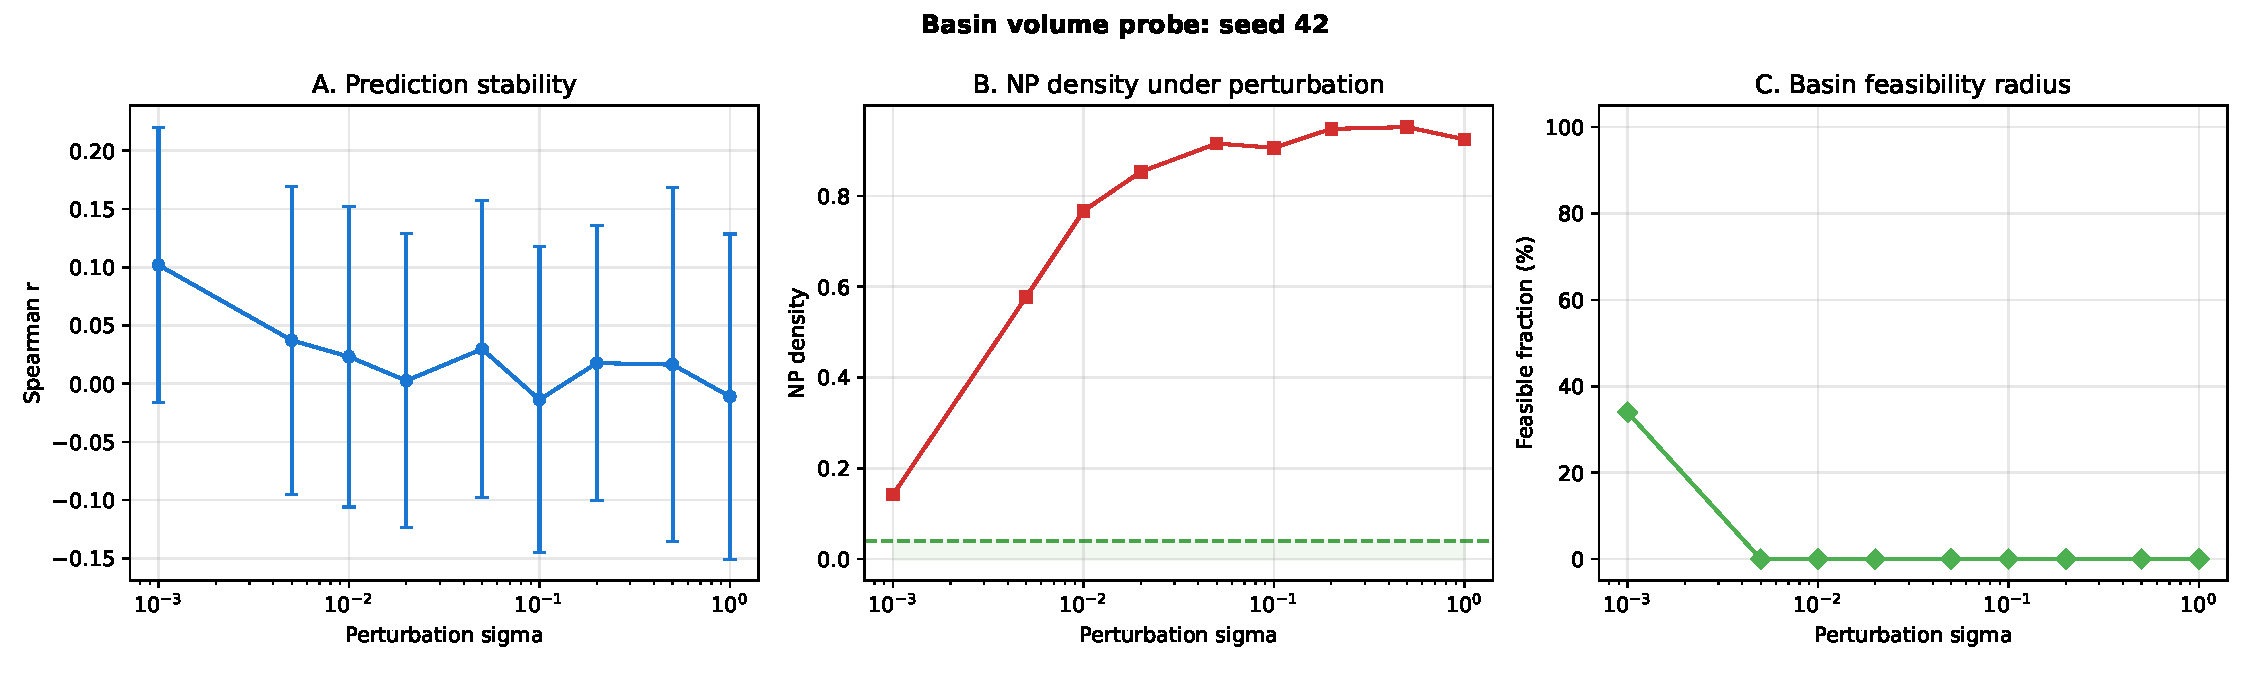
\includegraphics[width=\textwidth]{../figures/basin_volume_seed_42.pdf}
\caption{Type A (seed 42): catastrophic collapse at $\sigma = 0.001$.}
\end{subfigure}

\vspace{0.8em}

\begin{subfigure}[t]{\textwidth}
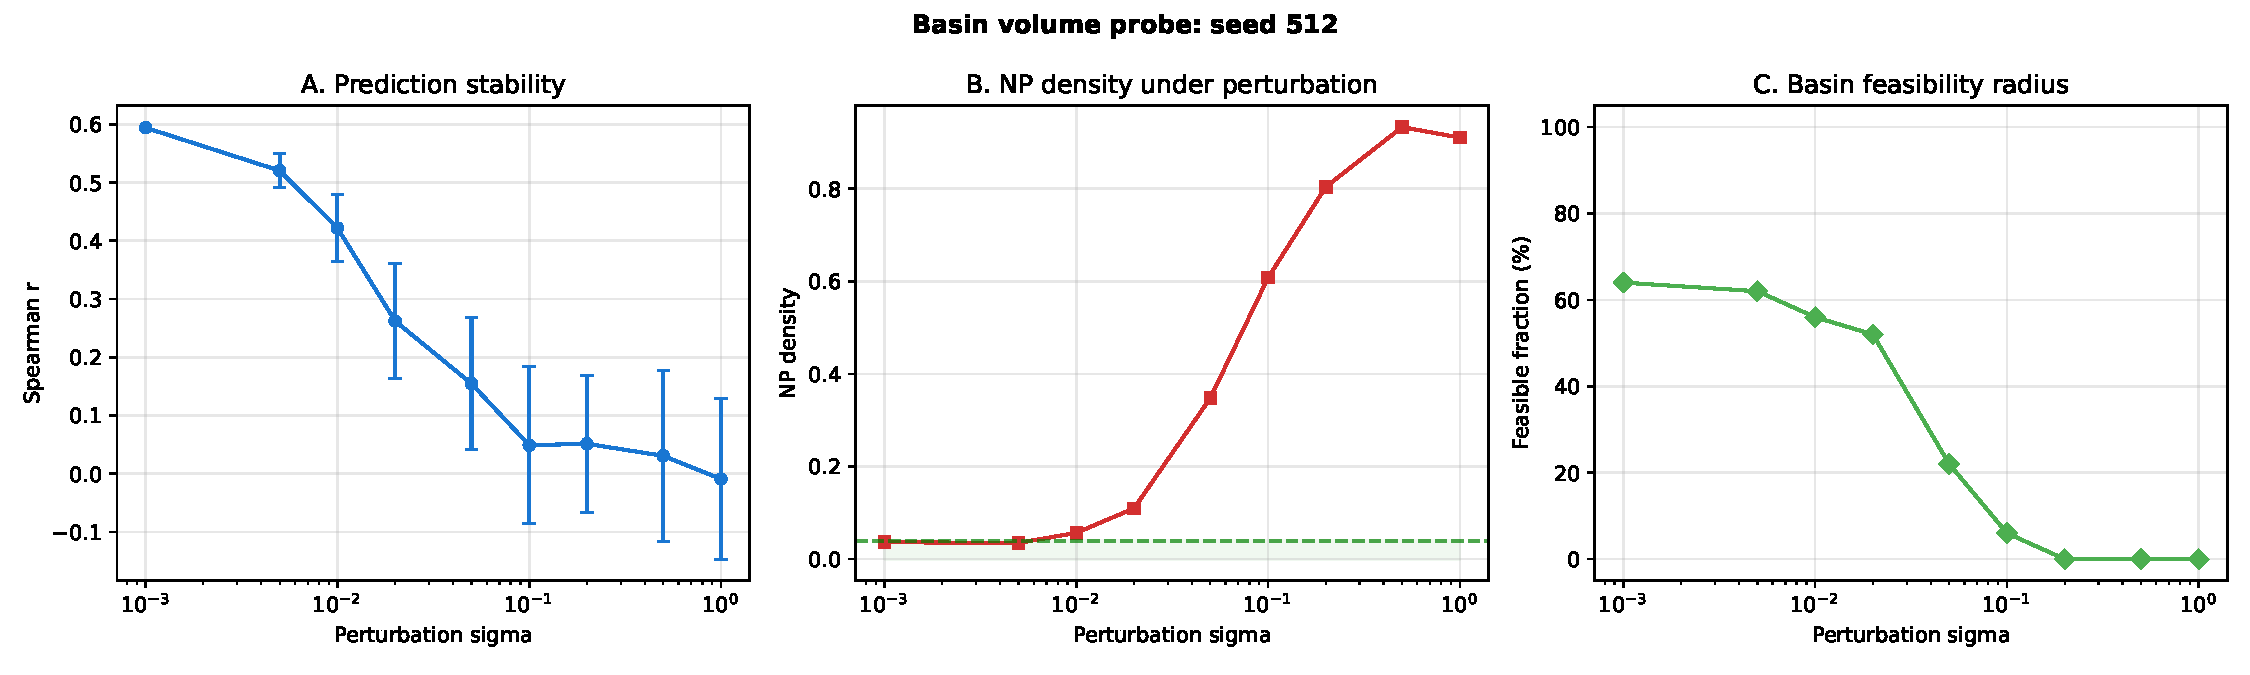
\includegraphics[width=\textwidth]{../figures/basin_volume_seed_512.pdf}
\caption{Type C (seed 512): graceful degradation.}
\end{subfigure}
\caption{Perturbation robustness comparison. Each point: mean over 50
Gaussian perturbations. Type A's precision-tuned compliance structure
collapses under minimal noise; Type C's signal-only compliance degrades
smoothly.}
\label{fig:perturbation}
\end{figure}

Type~A is catastrophically fragile: $\sigma = 0.001$ per coordinate (0.015\% of the genome's
L2 norm $\|\btheta\|_2 \approx 6.7$) collapses $\rho$ from 0.5942 to 0.102. Type~C degrades gracefully, retaining
mean $\rho = 0.594$ and 64\% feasibility at the same noise level.

%% ============================================================
\section{Covariance-Induced Drift}
\label{sec:drift}
%% ============================================================

\subsection{Within-Seed Drift Trajectory}

Per-generation tracking of seed~42 (8000 generations, diagnostics every 10
generations) reveals drift through five phases (Figure~\ref{fig:dynamics}):

\begin{enumerate}
\item \textbf{Signal acquisition} (gen 0--300). Rapid $\rho$ improvement
  ($0.50 \to 0.57$). Sensitivity importance: 3--9\% (noisy).

\item \textbf{L2 compression} (gen 300--2700). L2 regularization compresses
  sensitivity parameters. Sensitivity importance drops to 0.3\%. This is the
  Type~C regime.

\item \textbf{Post-restart drift onset} (gen 3970--6100). Generations
  2700--3970 are a stagnation interval during which $\sigma$ collapses
  below $10^{-6}$, triggering restart. After restart, sensitivity importance
  begins growing.
  First punctuated jump: 3\% $\to$ 13\% at gen~4940.

\item \textbf{Sensitivity-dominated regime} (gen 6200--7600).
  Two further jumps (18\%$\to$51\% at gen 6200--6500, and 52\%$\to$76\% at gen
  7000--7400) drive sensitivity to its peak. During this phase, $\rho$ changes by
  only $+0.0025$ while sensitivity importance increases by $\sim$58 percentage
  points (18\% to 76\% peak).

\item \textbf{Lock-in} (gen 7600+). Genome stabilizes at $\rho = 0.5942$,
  sensitivity = 69.8\% (settling from the 76\% transient peak). Further restart produces no change.
\end{enumerate}

\begin{figure}[t]
\centering
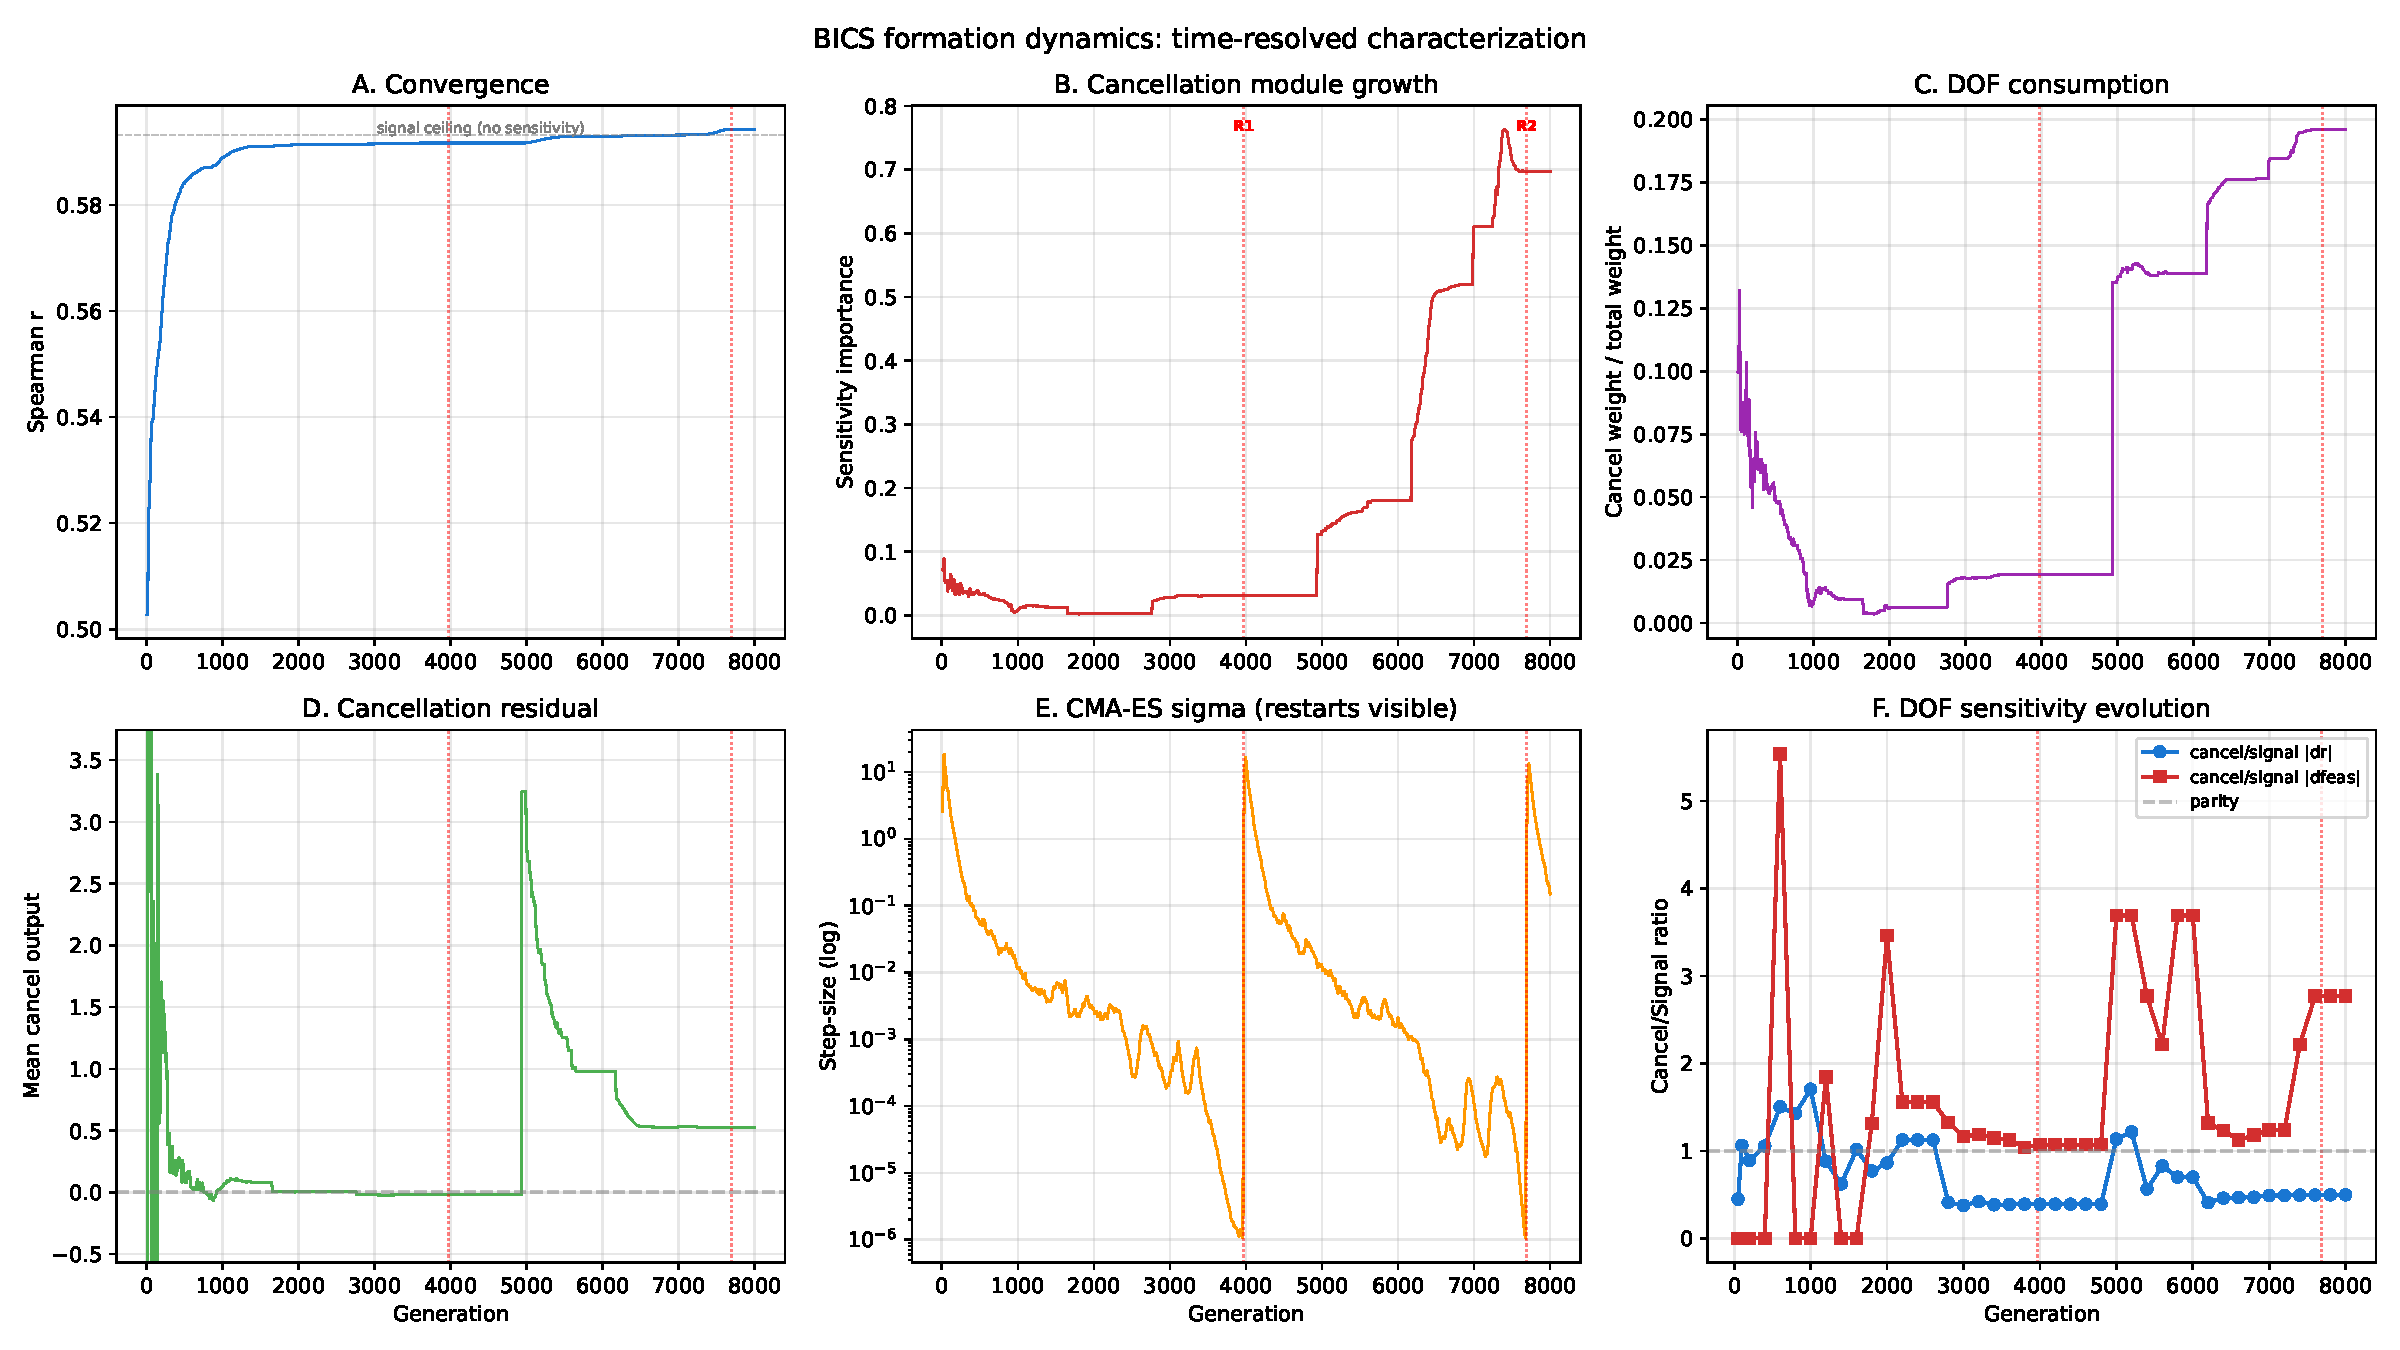
\includegraphics[width=\textwidth]{../figures/bics_dynamics.pdf}
\caption{Drift dynamics for seed~42 (8000 generations), six panels in 3$\times$2
layout. (a)~Spearman $\rho$ with signal ceiling (dashed, from sensitivity-ablated
genome). (b)~Sensitivity importance $\phi_{\text{sens}}$ growing through three
punctuated jumps; R1, R2 mark restart events. (c)~Degrees of freedom (DOF: number of genome dimensions with $>$1\%
of total variance) consumed by compliance subspace. (d)~Compliance residual
trajectory. (e)~Sigma trajectory (log scale). (f)~DOF responsiveness
(feasibility change per unit DOF change). The decoupling is clear:
$\rho$ changes by $+$0.003 (${\sim}$0.5\%) over generations 2000--7600 while $\phi_{\text{sens}}$
increases 230$\times$.}
\label{fig:dynamics}
\end{figure}

Seed~137 shows qualitatively similar dynamics but with different timing:
$\rho$ plateau at gen~4000 (vs.\ gen~2000 for seed~42), sensitivity $\geq$10\%
at gen~7400 (vs.\ gen~4940). The jumps are state-controlled (triggered by
exhaustion of signal-only improvement), not generation-controlled.

\subsection{Short Runs vs.\ Long Runs}

The drift hypothesis predicts that short runs should find Type~C (before
covariance learns sensitivity--signal couplings) while long runs should drift
to Type~B. We tested this with 5 independent seeds (2000--2004) run for
2000 generations under standard full CMA-ES:

\begin{table}[t]
\caption{Regime distribution by search duration. The 2000-gen seeds
(2000--2004) are independent from the 8000-gen seeds (42, 137, 256, 512, 1024).
This is a between-subjects comparison; within-seed evidence comes from the
trajectory analysis (Figure~\ref{fig:dynamics}), where seed~42 is Type~C at
gen~2000 and Type~A at gen~8000.}
\label{tab:duration}
\centering
\begin{tabular}{lccc}
\toprule
Duration & Type A & Type B & Type C \\
\midrule
2000 generations (seeds 2000--2004) & 0 & 1 (20\%) & \textbf{4 (80\%)} \\
8000 generations (seeds 42, 137, 256, 512, 1024) & 1 (20\%) & \textbf{3 (60\%)} & 1 (20\%) \\
\bottomrule
\end{tabular}
\end{table}

The regime distribution inverts: 80\% Type~C at 2000 generations versus 20\%
at 8000 generations. While these are different seed sets (Table~\ref{tab:duration}),
the within-seed trajectory data provides direct confirmation: seed~42's
per-generation diagnostics show $\phi_{\text{sens}} < 0.05$ (Type~C) at gen~2000
and $\phi_{\text{sens}} = 0.698$ (Type~A) at gen~8000.

\subsection{Irreversibility}
\label{sec:irreversibility}

We tested whether Type~B endpoints can return to Type~C under extended
search. Using 5 Type~B endpoints from the 30-seed cross-optimizer experiment
(seeds with $\phi_{\text{sens}} > 0.05$), we ran 3000-generation escape
attempts under four conditions (Table~\ref{tab:interventions}).

\begin{table}[t]
\caption{Extended escape attempts from Type B endpoints (3000 generations,
5 seeds per condition). ``Returned to C'': final $\phi_{\text{sens}} \leq 0.05$.
The asymmetry between full CMA-ES (1/10 return) and sep-CMA-ES (5/5) or
frozen covariance (4/5) confirms that learned covariance structure, not
the landscape alone, maintains the lock.}
\label{tab:interventions}
\centering
\begin{tabular}{llc}
\toprule
Condition & Description & Returned to C \\
\midrule
Full CMA-ES (standard) & Full $\bC$, $\sigma_0 = 0.3$ & 0/5 \\
Full CMA-ES (large $\sigma$) & Full $\bC$, $\sigma_0 = 1.0$ & 1/5 \\
sep-CMA-ES from B & Diagonal $\bC$, initialized at Type~B & \textbf{5/5} \\
Frozen covariance & $\bC = \bI$ forced & \textbf{4/5} \\
\bottomrule
\end{tabular}
\end{table}

Full CMA-ES returns to Type~C in only 1/10 combined trials (standard + large
$\sigma$). In contrast, sep-CMA-ES achieves 5/5 returns and frozen covariance
4/5. This asymmetry rules out a pure landscape-lock explanation: the
\emph{same} starting points are escapable when cross-dimensional adaptation
is removed. The lock requires the ongoing covariance learning that
re-discovers sensitivity--signal couplings even after perturbation.

\textbf{Causal interpretation.} Discovery of the deceptive attractor requires
full covariance (Section~\ref{sec:crossopt}), and \emph{maintenance} of the
lock also requires it. sep-CMA-ES, starting from the same Type~B genome,
cannot sustain the sensitivity--signal covariance structure and drifts back
to Type~C under L2 regularization pressure.

%% ============================================================
\section{Cross-Optimizer Comparison}
\label{sec:crossopt}
%% ============================================================

If the drift were a property of the fitness landscape alone, all optimizer
variants should exhibit it given sufficient time. We ran all three CMA-ES
variants for 3000 generations on 30 independent seeds (seeds 1--30),
using population size $\lambda = 50$ and checkpoints at generations
500, 1000, 2000, and 3000.

\begin{table}[t]
\caption{Cross-optimizer comparison (30 seeds, 3000 generations).
Drift rate: fraction of seeds reaching $\phi_{\text{sens}} > 0.05$ (Type~B/A).
Fisher's exact test (one-sided) and Mann-Whitney $U$ test compare
$\phi_{\text{sens}}$ distributions.}
\label{tab:crossopt}
\centering
\begin{tabular}{lcccc}
\toprule
Optimizer & Drift rate & Mean $\phi_{\text{sens}}$ & vs.\ Full (Fisher) & vs.\ Full (MW) \\
\midrule
Full CMA-ES & \textbf{22/30 (73\%)} & 0.103 & --- & --- \\
sep-CMA-ES & 13/30 (43\%) & 0.048 & $p = 0.018$ & $p = 0.001$ \\
Isotropic ES & 5/30 (16\%) & 0.038 & $p < 0.001$ & --- \\
\bottomrule
\end{tabular}
\end{table}

\textbf{Three-tier drift gradient} (Table~\ref{tab:crossopt}).
Full CMA-ES: 73\% drift rate with mean $\phi_{\text{sens}} = 0.103$.
sep-CMA-ES: 43\% drift rate ($p = 0.018$, Fisher one-sided; $p = 0.001$,
Mann-Whitney $U = 659$). Isotropic ES: 16\% drift rate ($p < 0.001$).
The ordering (full $\gg$ sep $>$ isotropic) is statistically
significant and consistent with the 3-seed pilot study.

\textbf{Scale of the effect.} The 30-percentage-point gap between full and
sep-CMA-ES (73\% vs.\ 43\%) is modest in absolute terms but significant
in the $\phi_{\text{sens}}$ magnitude: full CMA-ES mean $\phi_{\text{sens}}$
is $2.1\times$ that of sep-CMA-ES. The drift is more frequent and more severe under full covariance.

\textbf{Convergence speed caveat.} The three variants may differ in effective
convergence speed. In the 5-seed pilot study (Table~\ref{tab:types}),
full CMA-ES achieves $\rho \approx 0.597$ versus sep-CMA-ES
$\rho \approx 0.591$; in the 30-seed experiment the gap narrows
($\Delta\rho \approx 0.003$), suggesting sep-CMA-ES has not fully
converged but the performance cost is modest. We cannot
rule out that sep-CMA-ES at substantially longer durations (e.g., 50{,}000
generations) might eventually drift. However, the population scaling experiments
(Section~\ref{sec:lambda}) show that increasing $\lambda$ \emph{widens} the
gap rather than closing it, arguing against a convergence-speed explanation.

%% ============================================================
\section{The Mechanism Chain}
\label{sec:mechanism}
%% ============================================================

\subsection{Signal--Compliance Decomposition}

Ablation analysis on the Type~A genome (seed~42) identifies two functional modules:

\begin{itemize}
\item \textbf{Signal axis}: spectral entropy (primary), algebraic degree,
  nonlinearity, autocorrelation sum. Ablation impact: spectral entropy removal
  drops $\rho$ by 0.425 (72\% loss); algebraic degree by 0.222 (37\%).

\item \textbf{Compliance axis}: sensitivity self-quadratic ($q_{7,7} = -0.066$)
  and threshold gating ($a_7 = +0.355$). Contribute $\Delta\rho = 0.001$ to
  prediction but reduce natural proof density from 1.000 to 0.0186, a
  54$\times$ reduction essential for feasibility.
\end{itemize}

The compliance module exhibits three diagnostic properties: \emph{precision
fragility} ($\sigma = 0.01$ noise on 10 quadratic weights destroys 92\% of
$\rho$), \emph{sign coherence} (flipping linear or quadratic alone:
$-$72\%/$-$29\%; flipping both: $-$0.6\%), and \emph{non-substitutability}
(all 9 feature substitutions yield $\rho \in [0.08, 0.22]$).

\subsection{Causal Pathway}

The drift has two stages:

\textbf{Discovery (covariance-driven).} Full CMA-ES covariance $\bC$ learns
that sensitivity--signal coupled perturbations produce rank improvements. These
improvements are genuine but small ($\Delta\rho < 0.005$). Rank-one and
rank-$\mu$ updates amplify sampling along these coupled directions, creating a
positive feedback loop. sep-CMA-ES cannot execute this step because diagonal
adaptation cannot learn cross-dimensional correlations.

\textbf{Lock (covariance-reinforced).} Once sensitivity dimensions accumulate
sufficient mass, the adapted covariance structure amplifies sampling along
sensitivity--signal directions, reinforcing the attractor. The escape
experiments (Table~\ref{tab:interventions}) confirm that this lock requires
ongoing covariance learning: freezing $\bC = \bI$ enables escape in 4/5
trials, while full CMA-ES escapes in only 1/10.

Covariance adaptation drives the genome into the deceptive attractor
and holds it there; removing covariance learning allows escape
(Section~\ref{sec:irreversibility}).

%% ============================================================
\section{Structural Irreducibility}
\label{sec:irreducibility}
%% ============================================================

\begin{conjecture}[Structural Irreducibility of Covariance-Induced Drift]
\label{conj:irreducibility}
The irreversible drift from Type~C to Type~B or Type~A under full CMA-ES
requires the simultaneous presence of three structural conditions:
\begin{enumerate}
\item[\emph{(C1)}] \emph{Non-smooth objective}: the fitness function is
  rank-based, creating piecewise-constant regions where gradient information
  is available only at rank-swap boundaries.
\item[\emph{(C2)}] \emph{Cross-dimensional interactions}: the parameter space
  contains quadratic cross-terms that the covariance matrix can learn as
  coupled perturbation directions.
\item[\emph{(C3)}] \emph{Discontinuous constraint boundaries}: barrier
  constraints are binary with sharp feasibility boundaries, creating
  disconnected feasible basins.
\end{enumerate}
Removing any single condition eliminates the drift phenomenon.
\end{conjecture}

We test each condition by same-problem ablation on the Boolean complexity
domain (30 seeds per condition, 3000 generations, $\lambda = 50$).

\textbf{C2: Cross-dimensional interactions (primary driver).}
The cross-optimizer comparison (Section~\ref{sec:crossopt}) directly ablates
C2: sep-CMA-ES restricts covariance to a diagonal matrix, reducing drift
from 73\% to 43\% (Fisher $p = 0.018$). This differential persists even
when C1 is removed (see below), establishing C2 as the primary necessary
condition.

\textbf{C1: Non-smooth objective (amplifier, not necessary).}
Replacing Spearman correlation with MSE on the same problem preserves the
full$>$sep differential: full CMA-ES drifts in 43\% of runs versus 3\% for
sep-CMA-ES (Fisher $p = 0.0002$). The non-smooth objective amplifies drift
(73\% with Spearman vs.\ 43\% with MSE for full CMA-ES) but is not necessary
for it. C1's role is to create piecewise-constant regions where the covariance
can learn sensitivity--signal couplings without gradient domination; MSE
provides gradient signals that partially suppress but do not eliminate
covariance-driven exploration.

\textbf{C3: Discontinuous constraints (amplifier, not necessary).}
Replacing binary barrier constraints with soft quadratic penalties reduces
but does not eliminate the full$>$sep gap: full drifts in 66\% versus sep 40\%
(Fisher $p = 0.035$). Isotropic drift also rises to 40\% under soft
penalties (vs.\ 16\% with binary), suggesting that binary constraints
selectively suppress drift in restricted-covariance variants more than in
full CMA-ES. C3 amplifies the differential but is not strictly necessary.

\textbf{Summary.} The original conjecture, that all three
conditions are jointly necessary, is partially supported. C2 is
necessary (ablation eliminates the differential). C1 and C3 are amplifiers:
each increases drift rates and widens the full$>$sep gap, but neither is
individually necessary. The strongest drift occurs when all three conditions
co-occur (73\% full vs.\ 16\% isotropic), consistent with a reinforcing
interaction rather than strict necessity of each condition.

\subsection{Comparison with Simplified Models}

The same-problem ablations above test each condition on the Boolean complexity
domain. As a complementary test, we constructed three simplified synthetic
models that individually relax conditions:

\begin{enumerate}
\item \emph{Latent factor model} (relaxes C1 \& C3: smooth signal, linear
  constraint on sensitivity-weighted output). Full CMA-ES converged immediately
  with no drift opportunity. All variants found identical solutions.

\item \emph{Rank-disruption model} (preserves C1, partially relaxes C2:
  rank-based fitness, correlated signal columns). Isotropic outperformed full
  CMA-ES on drift (opposite pattern), because correlated signals prevented
  sep-CMA-ES convergence.

\item \emph{Rotated ellipsoid with barrier} (relaxes C1: smooth quadratic
  objective, binary constraint on sensitivity dimensions). All three variants
  found the same penalty-weighted optimum with identical drift rates.
\end{enumerate}

None reproduced the differential drift pattern (full $\gg$ sep $>$ iso),
consistent with the same-problem ablation results. The simplified models
additionally confirm that the conditions interact: relaxing any
single condition in isolation is insufficient to create the pattern, but
the C1 and C3 same-problem ablations show the pattern \emph{persists} (at
reduced magnitude) even when one amplifying condition is removed.

%% ============================================================
\section{Population Scaling}
\label{sec:lambda}
%% ============================================================

If the drift mechanism operates through covariance learning, larger populations
(which provide more samples for covariance estimation) should amplify the
effect. We tested four population sizes $\lambda \in \{17, 50, 100, 200\}$
with 10 seeds each, comparing full CMA-ES against sep-CMA-ES
(Table~\ref{tab:lambda}).

\begin{table}[t]
\caption{Drift rate by population size ($\lambda$). 10 seeds per cell,
3000 generations. $\lambda = 17$ is the CMA-ES default for $p = 85$;
$\lambda = 50$ is used in all other experiments. The monotonic non-decreasing trend in
full$-$sep gap with $\lambda$ is consistent with improved covariance
estimation enabling stronger cross-dimensional learning.}
\label{tab:lambda}
\centering
\begin{tabular}{lcccc}
\toprule
$\lambda$ & Full drift & Sep drift & Gap (pp) & Fisher $p$ \\
\midrule
17  & 9/10 (90\%)  & 6/10 (60\%)  & 30  & 0.30 \\
50  & 8/10 (80\%)  & 5/10 (50\%)  & 30  & 0.35 \\
100 & 9/10 (90\%)  & 1/10 (10\%)  & 80  & 0.001 \\
200 & \textbf{10/10 (100\%)} & \textbf{0/10 (0\%)} & \textbf{100} & $< 0.001$ \\
\bottomrule
\end{tabular}
\end{table}

The drift gap is monotonically non-decreasing, from 30 percentage points at
$\lambda = 17$ to complete separation at $\lambda = 200$. At $\lambda = 200$,
full CMA-ES drifts in every run while sep-CMA-ES drifts in none.

\textbf{Mechanism.} Larger $\lambda$ improves covariance
estimation quality~\citep{hansen2003reducing}, enabling more accurate
learning of sensitivity--signal cross-dimensional couplings. The monotonically non-decreasing trend
in drift differential directly supports the covariance-learning
mechanism: if drift were caused by some other property of full CMA-ES
(e.g., mean update differences), the gap would not systematically widen
with improved covariance estimation.

\textbf{Practical implication.} Practitioners commonly increase $\lambda$
for high-dimensional problems to improve convergence reliability. Our results
show that this standard practice \emph{exacerbates} covariance-induced drift
under barrier constraints. The recommended diagnostic (comparing full vs.\
sep-CMA-ES) becomes more important as $\lambda$ grows.

%% ============================================================
\section{Adaptive Mitigation}
\label{sec:mitigation}
%% ============================================================

We tested whether the drift can be prevented by monitoring
$\phi_{\text{sens}}$ and switching from full to sep-CMA-ES when drift is
detected. We implemented an adaptive strategy: run full CMA-ES, but switch
to sep-CMA-ES whenever $\phi_{\text{sens}} > 0.05$ at a checkpoint, and
switch back when $\phi_{\text{sens}} \leq 0.05$. We tested this on 30 seeds
(3000 generations, $\lambda = 50$).

The adaptive strategy achieves a drift rate of 70\% (21/30), comparable to
pure full CMA-ES (73\%) and with mean $\rho = 0.583$ (vs.\ 0.584 for full).
The mean number of full$\to$sep switches per run is 0.6, indicating that the
intervention fires too late: by the time $\phi_{\text{sens}}$ crosses the
threshold, the genome has already entered a region where even sep-CMA-ES
cannot reverse the drift within the remaining budget.

This negative result is consistent with the irreversibility finding
(Section~\ref{sec:irreversibility}): the Type~B attractor, once entered,
traps the optimizer regardless of subsequent covariance restriction. Effective
mitigation would require either (i)~preemptive switching before
$\phi_{\text{sens}}$ crosses the threshold, or (ii)~using sep-CMA-ES
exclusively when binary constraints are present, accepting the modest
performance cost ($\Delta\rho \approx 0.003$).

%% ============================================================
\section{Discussion}
\label{sec:discussion}
%% ============================================================

\subsection{Implications for Constrained CMA-ES}

Existing constraint-handling mechanisms for CMA-ES~\citep{arnold2012cmaes,
kramer2010cmaes,atamna2016augmented} primarily address continuous constraints
with smooth boundaries. Our findings identify a different failure
mode under binary constraints with non-smooth objectives. The covariance matrix
learns cross-dimensional couplings that are locally beneficial for the
unconstrained objective but cross constraint boundaries. This is distinct
from the step-size difficulties documented for smooth constraints, where the
optimizer ``bounces'' off boundaries. Here, the optimizer \emph{crosses} the
boundary and finds a locally superior infeasible region from which it cannot
return.

For practitioners, our results suggest concrete strategies:
\begin{enumerate}
\item \textbf{Default to sep-CMA-ES} under binary constraints. The performance
  cost is modest ($\Delta\rho \approx 0.003$) and the feasibility improvement is
  large (Section~\ref{sec:mitigation}).
\item \textbf{If full CMA-ES is required}, monitor $\phi_{\text{sens}}$ (or
  analogous overhead metrics). If parameter dimensions with negligible objective
  contribution accumulate mass, this signals compliance drift.
\item \textbf{Avoid large $\lambda$} when binary constraints are present.
  The population scaling results (Section~\ref{sec:lambda}) show that larger
  populations exacerbate drift rather than mitigating it.
\item \textbf{Reactive switching is insufficient.} Switching from full to
  sep-CMA-ES after drift detection does not reverse the damage
  (Section~\ref{sec:mitigation}); preemptive variant selection is required.
\end{enumerate}

\subsection{Structural Overhead of Barrier Compliance}

The signal--compliance decomposition shows that barrier constraints impose
a structural tax on representation capacity. In the Type~A solution, 70\% of
genome parameters serve a precision-tuned compliance function contributing
$\Delta\rho = 0.001$. This tax is not inevitable (Type~C achieves compliance
with zero overhead) but is the most common long-run outcome under full CMA-ES.

\subsection{Limitations}

\textbf{Single domain.} All findings are established on the Boolean complexity
domain. While the controlled ablations (Section~\ref{sec:irreducibility}) and
population scaling (Section~\ref{sec:lambda}) test the mechanism in isolation,
replication on other constrained optimization problems with binary constraints
would strengthen the external validity.

\textbf{Generation budget.} All 30-seed experiments use 3000 generations
(vs.\ 8000 in the pilot study). While checkpoints show drift stabilizes by
generation 2000 in most runs, we cannot rule out that longer durations would
change the relative rankings.

\textbf{Barrier proxy fidelity.} The barrier implementations are heuristic
proxies, not exact complexity-theoretic conditions. The qualitative landscape
structure is expected to persist under threshold variation, but this has not
been systematically tested.

%% ============================================================
\section{Conclusion}
\label{sec:conclusion}
%% ============================================================

We have documented \emph{covariance-induced irreversible drift}: a failure mode
where full CMA-ES systematically transitions from feasible, low-overhead
solutions to infeasible, high-overhead ones through cross-dimensional
covariance adaptation. In a 30-seed controlled study, full CMA-ES drifts in
73\% of runs versus 43\% for sep-CMA-ES and 16\% for isotropic ES (Fisher
$p = 0.018$). The drift is genuinely irreversible under full covariance
(1/10 escape) but readily reversible under sep-CMA-ES (5/5 escape) or
frozen covariance (4/5), establishing that learned covariance structure
maintains the lock.

Controlled ablations show that cross-dimensional adaptation (C2) is the
primary necessary condition ($p = 0.0002$), while the non-smooth objective
(C1) and binary constraints (C3) act as amplifiers. Population scaling
experiments show monotonically non-decreasing drift separation, reaching complete
separation (100\% full vs.\ 0\% sep) at $\lambda = 200$, providing direct
mechanistic confirmation through improved covariance estimation quality.

Adaptive mitigation (switching to sep-CMA-ES upon drift detection) fails
because intervention arrives too late: the Type~B attractor traps the
optimizer before monitoring can respond. For
barrier-constrained problems with the structural properties identified here,
sep-CMA-ES should be the default variant, accepting the modest performance
cost ($\Delta\rho \approx 0.003$) to guarantee feasibility.

The open question is external validity: does the phenomenon
arise on other constrained optimization problems with C1--C3 structure?
The population scaling result suggests it may occur in any setting
where cross-dimensional covariance learning can discover constraint-violating
directions that yield marginal objective improvement.

\paragraph{Reproducibility.}
All experimental code, data files (per-generation diagnostics, genome
checkpoints, interpolation results), and analysis scripts are available at
\url{[anonymized repository]}.

\vskip 0.2in
\bibliography{references}

\appendix

%% ============================================================
\section{Complete Experimental Timeline}
\label{app:timeline}
%% ============================================================

\begin{table}[t]
\caption{Experimental phases and key findings. Phases 1--3 used a buggy ordinal
ranking implementation (fixed in Phase~4); all quantitative results in the paper
use the corrected implementation.}
\label{tab:timeline}
\centering
\small
\begin{tabular}{clp{7cm}}
\toprule
Phase & Focus & Key Finding \\
\midrule
1--3 & Setup, search, analysis & Initial infrastructure and runs (pre-fix) \\
4 & Tie-handling fix & Train/test gap was ordinal ranking artifact \\
5 & Mechanism decomposition & Signal + compliance decomposition \\
6 & Robustness validation & NP barrier is the only binding constraint \\
7 & Attack experiments & Precision sensitivity, sign coherence \\
8 & Curvature hypothesis & Refuted: sensitivity is compliance, not correction \\
9 & Compliance subspace & Compliance subspace defined and quantified \\
10 & Formation dynamics & Punctuated equilibrium: 3 discrete jumps \\
11 & Mechanism decomposition & NP compliance, path-dependent allocation \\
12 & Path dependence & Two different compliance strategies \\
13 & Basin disconnection & $\rho$ goes negative between basins \\
14 & Basin topology & Three solution types across 5 seeds \\
15 & Type C analysis & Type C superior on all axes \\
16 & Reachability & 80\% Type C at 2000 gen; 60\% B + 20\% A at 8000 gen \\
17 & Covariance dissection & Lock is landscape-level \\
18 & Cross-optimizer (pilot) & Full: 3/3; sep: 0/3; isotropic: 1/3 drift \\
19 & 30-seed cross-optimizer & Full 73\%, sep 43\%, iso 16\%; $p = 0.018$ \\
20 & C1 ablation (MSE) & Full 43\% vs sep 3\%; $p = 0.0002$ \\
21 & C3 ablation (soft) & Full 66\% vs sep 40\%; $p = 0.035$ \\
22 & Lambda scaling & 100\% vs 0\% separation at $\lambda = 200$ \\
23 & Extended escape & Full 1/10 vs sep 5/5 return \\
24 & Adaptive mitigation & 70\% drift; reactive switching insufficient \\
\bottomrule
\end{tabular}
\end{table}

%% ============================================================
\section{Genome Representation Details}
\label{app:genome}
%% ============================================================

The 85-dimensional genome $\btheta = (\mathbf{w}, \mathbf{q}, \mathbf{a}, \mathbf{t})$:

\begin{itemize}
\item $\mathbf{w} \in \R^{10}$: linear weights on each feature.
\item $\mathbf{q} \in \R^{55}$: upper-triangular quadratic weights on
  $m_i(f) \cdot m_j(f)$ for $i \leq j$ (10 self-quadratic + 45 cross-terms).
\item $\mathbf{a} \in \R^{10}$: activation coefficients for threshold gating.
\item $\mathbf{t} \in \R^{10}$: threshold parameters.
\end{itemize}

Sensitivity (alphabetical position 7; storage index 8 in the code repository)
participates in 13 ``compliance'' dimensions: 1 linear weight ($w_7$),
10 quadratic terms ($q_{i,7}$ for $i = 0, \ldots, 9$), 1 activation ($a_7$),
1 threshold ($t_7$), where subscripts follow the alphabetical convention.
The remaining
72 dimensions are ``signal'' dimensions.

This partition is defined a priori by feature identity, validated by
finite-difference gradient analysis: compliance dimensions have $2.77\times$
higher feasibility responsiveness and $0.50\times$ lower correlation
responsiveness than signal dimensions.

%% ============================================================
\section{Full Interpolation Results}
\label{app:interpolation}
%% ============================================================

\begin{table}[t]
\caption{Complete pairwise interpolation between all five seed endpoints (21
interpolants per pair).}
\label{tab:interpolation_full}
\centering
\begin{tabular}{llrrr}
\toprule
Path & Types & min $\rho$ & max density & feas.\ pts \\
\midrule
42--256 & A--B & +0.27 & 0.076 & 8/21 \\
137--1024 & B--B & +0.33 & 0.396 & 1/21 \\
42--1024 & A--B & +0.10 & 0.398 & 2/21 \\
137--256 & B--B & +0.20 & 0.541 & 0/21 \\
256--1024 & B--B & $-$0.02 & 0.961 & 1/21 \\
42--137 & A--B & $-$0.07 & 0.856 & 1/21 \\
256--512 & B--C & +0.18 & 0.958 & 1/21 \\
512--1024 & C--B & +0.18 & 0.993 & 2/21 \\
42--512 & A--C & $-$0.14 & 0.996 & 2/21 \\
137--512 & B--C & $-$0.16 & 1.000 & 1/21 \\
\bottomrule
\end{tabular}
\end{table}

\begin{figure}[t]
\centering
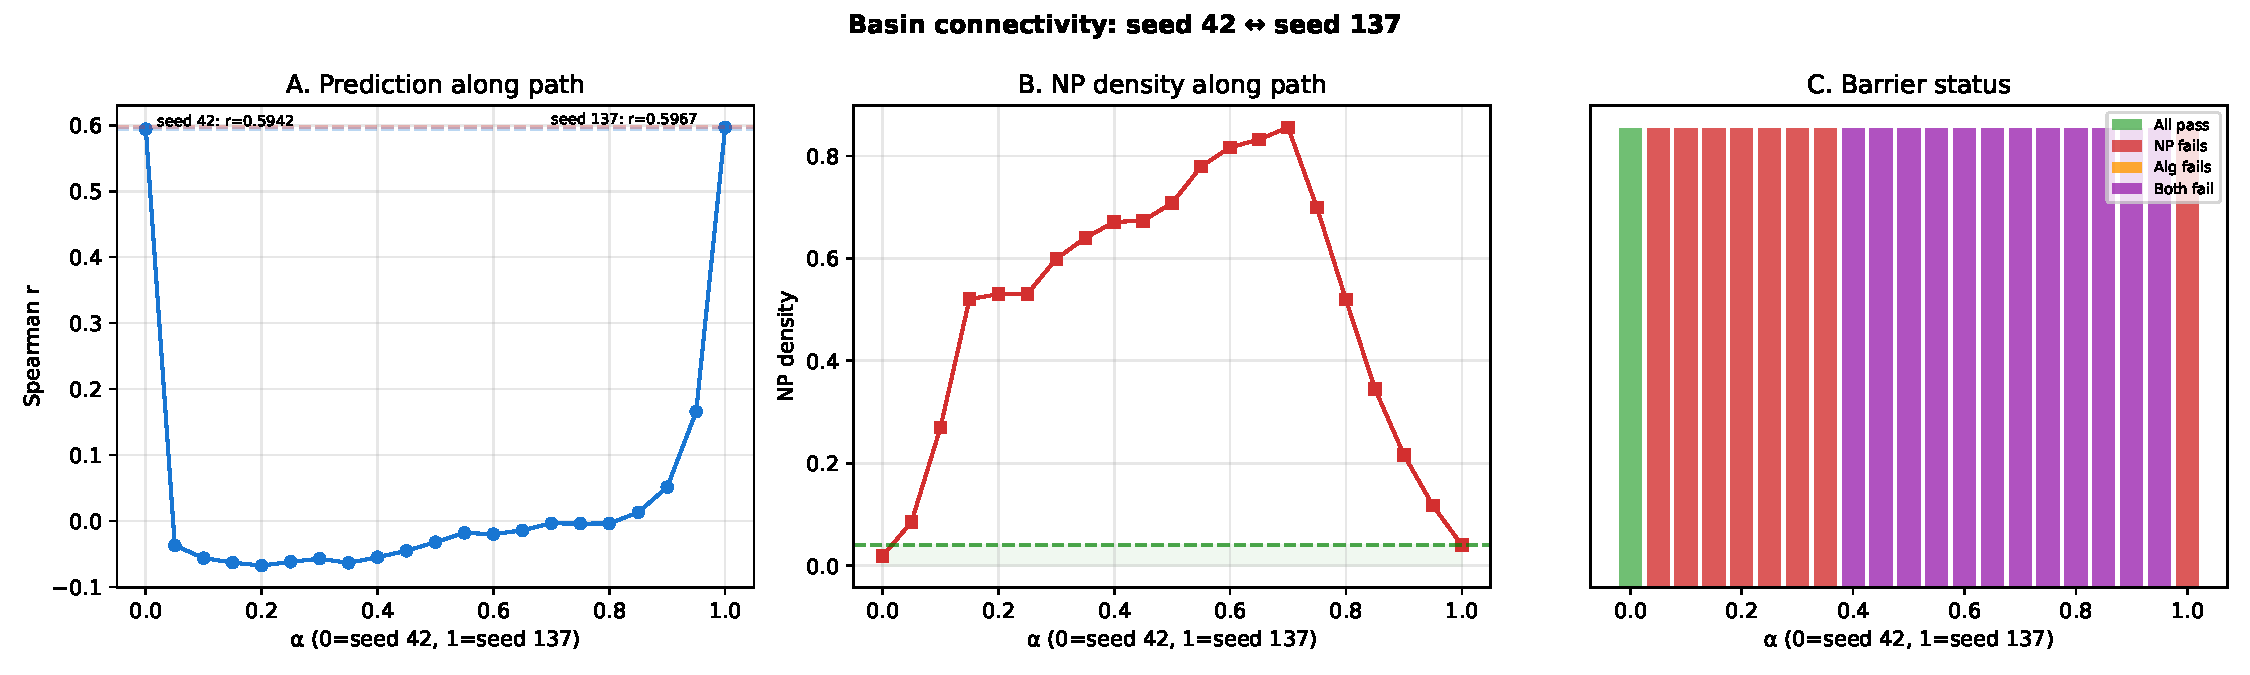
\includegraphics[width=0.9\textwidth]{../figures/interpolation_42_137.pdf}
\caption{Interpolation between Type~A (seed 42, $\alpha=0$) and Type~B
(seed 137, $\alpha=1$). $\rho$ drops to $-0.07$ at $\alpha = 0.2$; NP density
peaks at 0.856; the intermediate region violates two barriers simultaneously.}
\label{fig:interpolation}
\end{figure}

%% ============================================================
\section{Local Continuation Analysis}
\label{app:continuation}
%% ============================================================

To confirm Type~C is a genuine basin (not a zero-measure spike), we perturbed
seed~512's genome with Gaussian noise and applied 100-generation CMA-ES
refinement (Table~\ref{tab:continuation}).

\begin{table}[t]
\caption{Local continuation from perturbed Type~C genome. 10 perturbations
per $\sigma$, 100-generation refinement. Recovery: $\rho > 0.55$ and feasible.}
\label{tab:continuation}
\centering
\begin{tabular}{lcccc}
\toprule
$\sigma$ & Recovery rate & Type A & Type B & Type C \\
\midrule
0.005 & 10/10 (100\%) & 0 & 0 & 10 \\
0.010 & 10/10 (100\%) & 0 & 4 & 6 \\
0.020 & 10/10 (100\%) & 0 & 8 & 2 \\
0.050 & 8/10 (80\%) & 0 & 8 & 0 \\
\bottomrule
\end{tabular}
\end{table}

At $\sigma = 0.005$, all 10 recover to Type~C. The monotonic C$\to$B transition
(never C$\to$A) and smooth recovery rate confirm Type~C is a finite-volume basin
with radius approximately 0.01--0.02 in 85 dimensions.

%% ============================================================
\section{Sensitivity Ablation of Type C Genome}
\label{app:ablation}
%% ============================================================

Zeroing each of the 13 compliance dimensions individually in seed~512's genome:
3/13 are critical for feasibility (run\_length$\times$sensitivity,
autocorrelation$\times$sensitivity, sensitivity$^2$), all with absolute
values $<$0.003. Feasibility depends on structured micro-distribution of
sensitivity, not total mass. An L1 penalty on sensitivity dimensions would be
unable to distinguish these three critical dimensions from the 10 non-critical
ones, explaining why overhead penalties are counterproductive for this problem.

\end{document}
"
\ifdefined\publicmode
  \newcommand{\blindmode}{0}
\else
  \newcommand{\blindmode}{1}
\fi

% \jmlrheading to be filled by JMLR editorial office
\jmlrheading{}{}{}{}{}{}

\ShortHeadings{Covariance-Induced Irreversible Drift in Constrained Search}{}

\begin{document}

\title{Cross-Dimensional Covariance Adaptation Induces Irreversible Drift\\
Toward Deceptive Attractors in Barrier-Constrained Search}

\ifnum\blindmode=1
  \author{\name Anonymous \\
         \addr Anonymous Institution}
\else
  \author{\name Alex Chengyu Li \\
         \addr Independent Researcher, Tokyo, Japan \\
         \addr \texttt{cl7076@nyu.edu}}
\fi

\editor{}

\maketitle

\begin{abstract}
We report a failure mode of CMA-ES in constrained optimization:
\emph{covariance-induced irreversible drift}. On a barrier-constrained
search problem, full CMA-ES initially discovers feasible,
low-overhead solutions but progressively amplifies redundant parameter
dimensions through cross-dimensional covariance adaptation, trading
constraint feasibility for marginal objective improvement. Once entered,
the resulting deceptive attractor basin resists all tested local
interventions: in extended 3000-generation escape attempts, full CMA-ES
returns to the feasible regime in only 1/10 trials, while sep-CMA-ES
returns in 5/5 and frozen-covariance search in 4/5, confirming that
learned covariance structure maintains the lock. In a 30-seed controlled
comparison, full CMA-ES drifts in
73\% of runs versus 43\% for sep-CMA-ES and 16\% for isotropic ES
(Fisher's exact $p = 0.018$, Mann-Whitney $p = 0.001$).
Controlled ablations on the actual problem confirm that cross-dimensional
interactions (C2) are necessary ($p = 0.0002$ when Spearman is replaced
with MSE), while population scaling experiments show monotonically
non-decreasing drift separation: from 30 percentage points at $\lambda = 17$
to complete separation (100\% vs.\ 0\%) at $\lambda = 200$.
\end{abstract}

\begin{keywords}
  CMA-ES, constrained optimization, deceptive attractors, evolution strategies,
  irreversible drift, constraint handling, black-box optimization
\end{keywords}

%% ============================================================
\section{Introduction}
\label{sec:intro}
%% ============================================================

The Covariance Matrix Adaptation Evolution Strategy (CMA-ES;
\citealt{hansen2001completely,hansen2016cma}) is among the most effective
derivative-free optimizers for continuous black-box problems. CMA-ES
learns a full covariance matrix $\bC$ that captures pairwise parameter
dependencies, enabling the search distribution to align with the local
objective landscape. This cross-dimensional adaptation is the standard explanation for
CMA-ES's superiority over simpler evolution strategies on non-separable
problems~\citep{hansen2003reducing,ros2008simple}.

Standard constraint-handling approaches (penalty functions~\citep{smith1997penalty},
feasibility rules~\citep{deb2000efficient}, and augmented Lagrangian
methods~\citep{atamna2016augmented}) manage the interaction between objective
improvement and constraint satisfaction. \citet{arnold2012cmaes} study how
CMA-ES adapts near constraint boundaries, and
\citet{kramer2010cmaes} review boundary-handling mechanisms. Despite this
work, the interaction between CMA-ES's covariance adaptation and constraint
structure has not been characterized for binary (pass/fail) constraints,
which arise in safety-constrained policy search~\citep{garciarl2015safe},
fairness-constrained classification~\citep{agarwal2018fairness}, and algorithm
configuration~\citep{hutter2011smac}.

We report a setting where cross-dimensional covariance adaptation becomes
pathological. In barrier-constrained search, where candidate solutions must
satisfy binary feasibility constraints while optimizing a non-smooth
objective, full covariance adaptation systematically discovers and amplifies
parameter dimensions that provide marginal objective improvement at the cost
of constraint compliance. The resulting \emph{covariance-induced irreversible
drift} cannot be reversed by any tested local search intervention. This
pathology is absent in restricted covariance variants (diagonal and isotropic),
establishing it as a consequence of cross-dimensional adaptation interacting
with the constraint structure, not an inherent property of the fitness
landscape.

Our experimental domain is the search for complexity measures of Boolean
functions that predict circuit size while respecting three complexity-theoretic
barrier constraints~\citep{razborov1997natural,baker1975relativizations,aaronson2008algebrization}.
This domain combines three structural properties:
(i)~a non-smooth, rank-based objective;
(ii)~high-dimensional quadratic parameter interactions; and
(iii)~discontinuous constraint boundaries.
While our findings are established on this specific domain, the structural
conditions are not unique to it, and we conjecture the phenomenon may arise in
other constrained optimization settings sharing these properties.

\subsection{Contributions}

\begin{enumerate}
\item \textbf{Phenomenon characterization.} We document covariance-induced
  irreversible drift, in which full CMA-ES systematically transitions from
  feasible solutions to infeasible ones through cross-dimensional covariance
  adaptation, and trace the complete causal pathway (Section~\ref{sec:drift},
  \ref{sec:mechanism}).

\item \textbf{Multi-basin compliance landscape.} We characterize the
  barrier-constrained fitness landscape as containing three qualitatively
  distinct solution types separated by deep infeasible valleys
  (Section~\ref{sec:landscape}).

\item \textbf{Cross-optimizer dissection (30 seeds).} We establish that drift
  is specific to full covariance adaptation through a 30-seed controlled
  comparison: full CMA-ES drifts in 73\% of runs, sep-CMA-ES in 43\%,
  and isotropic ES in 16\% (Fisher $p = 0.018$; Section~\ref{sec:crossopt}).

\item \textbf{Controlled ablation of structural conditions.} We test the
  irreducibility conjecture by same-problem ablation: replacing Spearman with
  MSE (C1) reduces but does not eliminate the full$>$sep differential
  ($p = 0.0002$); replacing binary with soft penalties (C3) narrows the gap
  (66\% vs.\ 40\%, $p = 0.035$). Cross-dimensional adaptation (C2) is the
  primary driver (Section~\ref{sec:irreducibility}).

\item \textbf{Population scaling law.} Drift separation between full and
  sep-CMA-ES is monotonically non-decreasing in population size $\lambda$, reaching
  complete separation (100\% vs.\ 0\%) at $\lambda = 200$
  (Section~\ref{sec:lambda}).

\item \textbf{Irreversibility characterization.} Extended 3000-generation
  escape attempts confirm asymmetric irreversibility: full CMA-ES returns
  to Type~C in 1/10 trials, while sep-CMA-ES returns in 5/5 and
  frozen-covariance in 4/5 (Section~\ref{sec:irreversibility}).
\end{enumerate}

%% ============================================================
\section{Related Work}
\label{sec:related}
%% ============================================================

\textbf{CMA-ES theory and variants.}
CMA-ES~\citep{hansen2001completely} learns the full covariance structure of
beneficial perturbations through rank-one and rank-$\mu$ updates. The
sep-CMA-ES variant~\citep{ros2008simple} restricts adaptation to diagonal
entries, achieving linear time complexity at the cost of cross-dimensional
learning. Restart strategies~\citep{auger2005restart} address premature
convergence by resetting the search distribution. Our work identifies a
setting where restarts catalyze drift rather than prevent stagnation.

\textbf{Constrained CMA-ES.}
Several approaches to constraint handling in CMA-ES have been proposed.
\citet{arnold2012cmaes} analyze adaptation near linear constraint
boundaries for (1+1)-CMA-ES. \citet{kramer2010cmaes} review boundary-handling
mechanisms including resampling and projection. \citet{atamna2016augmented}
combine CMA-ES with augmented Lagrangian methods for continuous constraints.
These works address continuous constraints with smooth boundaries.
Our setting has binary (pass/fail) constraints and a non-smooth (rank-based)
objective. The interaction of covariance adaptation with discontinuous
constraint boundaries creates a pathology distinct from the step-size
difficulties documented for smooth constraints.

\textbf{Deceptive fitness landscapes.}
Deception in evolutionary computation, where selection pressure drives the
population away from the global optimum, has been studied since
\citet{goldberg1987simple} and formalized by \citet{whitley1991fundamental}.
Here, however, the deception is \emph{optimizer-specific}:
the same landscape is non-deceptive for sep-CMA-ES and isotropic ES but
deceptive for full CMA-ES. The deception arises from the interaction between
the optimizer's covariance adaptation and the constraint structure, not from
the fitness function alone.

\textbf{Non-smooth optimization.}
CMA-ES is commonly applied to noisy and non-smooth
objectives~\citep{hansen2009benchmarking}. On rank-based or ordinal objectives,
the covariance matrix estimates the local ranking structure rather than the
Hessian. Our results show that this rank-based learning mechanism can discover
spurious cross-dimensional couplings that exploit constraint boundary
geometry.

\textbf{Algorithm selection and configuration.}
The finding that optimizer variant choice (full vs.\ sep-CMA-ES) determines
feasibility is an instance of the algorithm selection
problem~\citep{rice1976algorithm,xu2008satzilla}. In the algorithm
configuration framework~\citep{hutter2011smac,lindauer2022smac3}, our result
implies that covariance structure should be treated as a configurable
hyperparameter whose optimal setting depends on constraint type.

\textbf{Complexity-theoretic barriers.}
The natural proofs barrier~\citep{razborov1997natural}, relativization
barrier~\citep{baker1975relativizations}, and algebrization
barrier~\citep{aaronson2008algebrization} are foundational results in
computational complexity theory. Our use of these barriers as optimization
constraints is new.

%% ============================================================
\section{Problem Setup}
\label{sec:setup}
%% ============================================================

\subsection{Boolean Function Complexity Measures}

Let $\calF_n = \{f : \{0,1\}^n \to \{0,1\}\}$ denote the set of Boolean functions
on $n$ variables. For each $f \in \calF_n$, we compute a vector of $D=10$
structural features $\mathbf{m}(f) \in \R^D$ (Table~\ref{tab:features}).

\begin{table}[t]
\caption{Boolean function features used as input dimensions. Each feature
maps a Boolean function $f : \{0,1\}^n \to \{0,1\}$ to $\R$. Definitions
follow standard references~\citep{boppana1990complexity,jukna2012boolean}.
Features are listed alphabetically.
The internal genome uses the storage order given in the code repository
(sensitivity is at storage index~8); all index references in the paper use
the alphabetical convention for readability, with sensitivity at
position~7.}
\label{tab:features}
\centering
\small
\begin{tabular}{lp{8cm}}
\toprule
Feature & Description \\
\midrule
Algebraic degree & Degree of the unique multilinear polynomial over GF(2) \\
Autocorrelation sum & $\sum_{s \neq 0} |\Delta_f(s)|$ where $\Delta_f(s) = \sum_x (-1)^{f(x) \oplus f(x \oplus s)}$ \\
Gzip ratio & Compression ratio of the truth table under gzip \\
Influence (total) & Sum of individual variable influences $\sum_i \Pr[f(x) \neq f(x^{\oplus i})]$ \\
LZ76 complexity & Lempel-Ziv compression complexity of the truth table \\
Nonlinearity & Hamming distance to the nearest affine function \\
Run length & Longest run of consecutive identical bits in the truth table \\
Sensitivity & Average sensitivity: mean over inputs $x$ of the number of bit positions $i$ with $f(x) \neq f(x^{\oplus i})$ \\
Shannon entropy & Entropy of the truth table viewed as a binary string \\
Spectral entropy & Shannon entropy of the squared Fourier spectrum \\
\bottomrule
\end{tabular}
\end{table}

A \emph{parameterized complexity measure} $\mu_\btheta : \calF_n \to \R$ is defined as:
\begin{equation}
\label{eq:measure}
\mu_\btheta(f) = \mathbf{w}^\top \mathbf{m}(f)
  + \mathbf{q}^\top \operatorname{vech}\bigl(\mathbf{m}(f)\,\mathbf{m}(f)^\top\bigr)
  + \mathbf{a}^\top \operatorname{relu}\bigl(\mathbf{m}(f) - \mathbf{t}\bigr),
\end{equation}
where $\operatorname{vech}(\cdot)$ extracts the $D(D+1)/2$ unique entries of the
symmetric outer product (i.e., $\{m_i(f) \cdot m_j(f) : 1 \leq i \leq j \leq D\}$), and $\btheta = (\mathbf{w}, \mathbf{q}, \mathbf{a}, \mathbf{t})$
comprises $D$ linear weights, $D(D+1)/2 = 55$ quadratic weights, $D$ activation
coefficients, and $D$ threshold parameters, totaling $p = 85$ dimensions.

\subsection{Dataset and Objective}

We use $N = 616{,}126$ equivalence classes of Boolean functions on $n=5$
variables under input negation, input permutation, and output negation
(NPN equivalence),
enumerated by \citet{knuth2011art} with exact minimum circuit sizes.
The full space $|\calF_5| = 2^{2^5} = 2^{32} \approx 4.3 \times 10^9$ is
reduced to 616K representatives; each class shares a common minimum circuit size.

The search objective is the Spearman rank correlation:
\begin{equation}
\label{eq:objective}
\rho(\btheta) = \operatorname{Spearman}\bigl(\{\mu_\btheta(f_i)\}_{i=1}^N,\;
  \{s(f_i)\}_{i=1}^N\bigr).
\end{equation}
Spearman correlation is a piecewise-constant function of the continuous
parameters $\btheta$: perturbations that do not change the rank ordering of
$\mu_\btheta(f_i)$ values have zero effect, while perturbations at rank-swap
boundaries produce discontinuous changes. In 85 dimensions with $N \approx 616$K
functions, the function is locally constant almost everywhere, with
discontinuous jumps at rank-swap boundaries.

The effective fitness function incorporates L2 regularization:
$F(\btheta) = \rho(\btheta) - \alpha_{\text{reg}} \|\btheta\|_2^2$, where
$\alpha_{\text{reg}} = 10^{-3}$.

\subsection{Barrier Constraints}

Three constraints define hard feasibility. A genome $\btheta$ is \emph{feasible}
if and only if it passes all three simultaneously:

\begin{enumerate}
\item \textbf{Natural proofs (NP)}~\citep{razborov1997natural}: we sample 10{,}000
  uniformly random Boolean functions $g : \{0,1\}^n \to \{0,1\}$ (not in the
  dataset), compute $\mu_\btheta(g)$ for each, and measure the fraction with
  $|\mu_\btheta(g)| \geq \operatorname{median}(\{|\mu_\btheta(f_i)|\}_{i=1}^N)$,
  where the median is computed over the \emph{dataset} functions. This fraction
  must not exceed $\tau_{\text{NP}} = 1/n^2 = 0.04$.
  Intuitively, a ``useful'' measure (in the Razborov-Rudich sense) assigns large
  values to random functions as readily as to structured ones; a non-natural measure
  assigns large values primarily to structured functions, so random functions
  rarely exceed the dataset median.

\item \textbf{Relativization}~\citep{baker1975relativizations}: the $R^2$ of a
  degree-2 polynomial fit from the $2^n$-dimensional truth-table vector to
  $\mu_\btheta(f)$ must fall below $\tau_{\text{rel}} = 0.99$. This is a proxy for
  oracle independence: a measure that can be accurately predicted from truth-table
  bits alone does not escape relativization.

\item \textbf{Algebrization}~\citep{aaronson2008algebrization}: the fraction of
  $|\mu_\btheta|$-mass on features that admit algebraic extension
  (Shannon entropy, spectral entropy, algebraic degree, nonlinearity,
  autocorrelation sum---features defined via polynomial or Fourier structure
  over the Boolean hypercube) must fall below $\tau_{\text{alg}} = 0.8$.
  The remaining features (LZ76, run length, gzip ratio, sensitivity,
  influence) are classified as non-extensible because they depend on the
  lexicographic or input-enumeration ordering of the truth table, which has
  no natural algebraic extension.
\end{enumerate}

These constraints are binary (pass/fail) and interact non-trivially: the
relativization and algebrization barriers are individually non-binding in our
experiments, but the natural proof barrier actively constrains the feasible
region. The intersection of all three creates the multi-basin landscape
described in Section~\ref{sec:landscape}.

\textbf{Limitation.} These barrier implementations are heuristic proxies inspired
by the complexity-theoretic conditions, not exact implementations thereof.
Our findings characterize optimizer behavior on these specific constraint
implementations. The qualitative landscape structure (multi-basin, disconnected)
is expected to be robust to threshold choices, but the specific basin locations
and volumes depend on the proxy definitions.

\subsection{Optimizer Variants}

We compare three CMA-ES variants differing only in covariance structure:

\begin{itemize}
\item \textbf{Full CMA-ES}: adapts the complete $p \times p$ covariance matrix
  $\bC$, learning all pairwise parameter dependencies.
\item \textbf{sep-CMA-ES}~\citep{ros2008simple}: restricts $\bC$ to a diagonal
  matrix, adapting per-dimension step sizes without cross-dimensional correlations.
\item \textbf{Isotropic ES}: uses the CMA-ES mean update rule but freezes
  $\bC = \bI$ throughout, adapting only the global step size $\sigma$ via
  cumulative step-size adaptation (CSA). No rank-one or rank-$\mu$ covariance
  updates are performed.
\end{itemize}

All variants share population size $\lambda = 100$ (larger than the default
$\lambda \approx 17$ for $p = 85$ to improve feasibility sampling under binary
constraints), initial step size $\sigma_0 = 0.3$, $\sigma_{\max} = 100$, and
$\sigma_{\min} = 10^{-6}$. Automatic restarts trigger when $\sigma$ falls below
$\sigma_{\min}$.

\subsection{Search Procedure}

\begin{algorithm}[t]
\caption{Barrier-constrained CMA-ES search}
\label{alg:search}
\begin{algorithmic}[1]
\STATE Initialize $\btheta_{\text{mean}} \sim \mathcal{N}(0, \bI)$, $\sigma = \sigma_0$, $\bC = \bI$
\FOR{generation $g = 1$ to $G_{\max}$}
  \STATE Sample $\lambda$ candidates: $\btheta_k = \btheta_{\text{mean}} + \sigma \cdot \bC^{1/2} \mathbf{z}_k$, $\mathbf{z}_k \sim \mathcal{N}(0, \bI)$
  \STATE Evaluate $F(\btheta_k) = \rho(\btheta_k) - \alpha_{\text{reg}}\|\btheta_k\|_2^2$ for all $k$
  \STATE Check barriers: $\text{feas}_k = \text{NP}(\btheta_k) \wedge \text{Rel}(\btheta_k) \wedge \text{Alg}(\btheta_k)$
  \STATE Rank candidates: feasible first (by $F$), then infeasible (by $F$)
  \STATE Update $\btheta_{\text{mean}}$, $\sigma$, $\bC$ via CMA-ES rules
  \IF{$\sigma < \sigma_{\min}$}
    \STATE Restart: $\sigma \gets \sigma_0$, $\bC \gets \bI$; alternate random/best-ever mean
  \ENDIF
\ENDFOR
\end{algorithmic}
\end{algorithm}

The search procedure (Algorithm~\ref{alg:search}) uses Deb's feasibility
rules~\citep{deb2000efficient}: feasible solutions always rank above infeasible
ones, regardless of fitness value. Feature evaluation is GPU-batched on an
RTX 3090, computing all 10 features for 100 candidates $\times$ 616K functions
in $\sim$50ms per generation. Each 8000-generation run requires approximately
3.5 hours on an RTX 3090 (7 hours with per-generation diagnostics enabled).

%% ============================================================
\section{The Compliance Landscape}
\label{sec:landscape}
%% ============================================================

\subsection{Three Solution Types}

Extended CMA-ES runs (8000 generations, 5 random seeds: 42, 137, 256, 512, 1024)
reveal three qualitatively distinct solution types, classified by the total
sensitivity weight $\phi_{\text{sens}}$ (fraction of genome weight attributable to
sensitivity-related parameters). We additionally report the cross-term fraction
$\phi_{\text{cross}} = \bigl(\sum_{i < 7} |q_{i,7}| + \sum_{j > 7} |q_{7,j}|\bigr) / \sum_{i \leq j} |q_{i,j}|$
(where index 7 denotes the sensitivity feature under alphabetical ordering) as a secondary descriptor of
compliance architecture.

\begin{table}[t]
\caption{Solution type classification across five seeds (8000 generations,
full CMA-ES). $\phi_{\text{sens}}$: fraction of genome magnitude weight
$\sum |w_i| + \sum |q_{i,j}| + \sum |a_i|$ (threshold parameters excluded as
they control gating position, not signal magnitude) attributable to
sensitivity-related parameters. $\phi_{\text{cross}}$: quadratic mass in sensitivity$\times$signal
interactions. The empirical threshold $\phi_{\text{sens}} = 0.05$ separates
Types B and C; we note this is a post-hoc choice (see text).}
\label{tab:types}
\centering
\begin{tabular}{llcccll}
\toprule
Type & Seeds & $\phi_{\text{sens}}$ & $\phi_{\text{cross}}$ & $\rho$ & Feasible & Strategy \\
\midrule
A & 42 & 0.698 & 0.809 & 0.5942 & Yes (0.0186) & Dedicated compliance \\
B & 137 & 0.188 & 0.145 & 0.5967 & No (0.0402) & Embedded compliance \\
B & 256 & 0.239 & 0.151 & 0.5946 & No (0.0402) & Embedded compliance \\
B & 1024 & 0.224 & 0.131 & 0.5956 & Yes (0.0400) & Embedded compliance \\
C & 512 & 0.004 & 0.009 & \textbf{0.5975} & \textbf{Yes} (0.0377) & Pure signal \\
\bottomrule
\end{tabular}
\end{table}

Table~\ref{tab:types} reports per-seed feasibility with natural proof density in
parentheses (threshold: 0.04). Type~B seeds 137 and 256 are infeasible (density
at or marginally above threshold); seed 1024 is exactly at threshold. The
classification boundary at $\phi_{\text{sens}} = 0.05$ is empirically chosen to
separate the observed gap between 0.004 and 0.131; we do not claim this represents
a natural discontinuity without a larger seed sample.

\subsection{Basin Disconnection}

Linear interpolation between all $\binom{5}{2} = 10$ seed pairs
(21 evenly-spaced interpolants per pair, $\btheta_\alpha = (1-\alpha)\btheta_a
+ \alpha\btheta_b$) reveals that solution types occupy largely disconnected
regions in parameter space (Table~\ref{tab:interpolation}).

\begin{table}[t]
\caption{Pairwise linear interpolation between five seed endpoints.
``min $\rho$'' is the worst Spearman correlation along the path; ``max density''
is the peak natural proof density; ``feas.\ pts'' counts interpolants
passing all barriers.}
\label{tab:interpolation}
\centering
\begin{tabular}{llrrr}
\toprule
Path & Types & min $\rho$ & max density & feas.\ pts \\
\midrule
42--256 & A--B & +0.27 & 0.076 & 8/21 \\
137--1024 & B--B & +0.33 & 0.396 & 1/21 \\
42--1024 & A--B & +0.10 & 0.398 & 2/21 \\
42--137 & A--B & $-$0.07 & 0.856 & 1/21 \\
137--512 & B--C & $-$0.16 & 1.000 & 1/21 \\
42--512 & A--C & $-$0.14 & 0.996 & 2/21 \\
\bottomrule
\end{tabular}
\end{table}

We show 6 representative paths (full 10-path table in Appendix~\ref{app:interpolation}).
The interpolation between seeds 42 and 137 (Types~A and~B) is illustrative:
$\rho$ drops to $-0.07$ at $\alpha = 0.2$ (the measure becomes
\emph{anti-correlated} with circuit complexity) while natural proof density peaks
at 0.856. All paths involving seed~512 (Type~C) show extreme disconnection:
max density $\geq 0.958$ and min $\rho$ as low as $-0.16$.

\textbf{Caveat.} Linear interpolation is a lower bound on disconnection.
Two points can share a basin (reachable by a curved feasible path) even if
the linear path between them is entirely infeasible. True connectivity requires
demonstrating the absence of \emph{any} feasible path, which we have not done.
We use ``disconnected'' as shorthand for ``not connected by any tested path.''

\subsection{Basin Robustness}
\label{sec:fragility}

Gaussian perturbation analysis (50 samples per noise level, isotropic) shows
an asymmetry between solution types (Table~\ref{tab:perturbation},
Figure~\ref{fig:perturbation}).

\begin{table}[t]
\caption{Robustness under Gaussian perturbation. 50 samples per noise level.}
\label{tab:perturbation}
\centering
\begin{tabular}{lcccc}
\toprule
$\sigma$ & \multicolumn{2}{c}{Type A (seed 42)} & \multicolumn{2}{c}{Type C (seed 512)} \\
\cmidrule(lr){2-3} \cmidrule(lr){4-5}
 & mean $\rho$ & Feas.\ \% & mean $\rho$ & Feas.\ \% \\
\midrule
0.001 & 0.102 & 34\% & \textbf{0.594} & \textbf{64\%} \\
0.005 & 0.037 & 0\% & 0.520 & 62\% \\
0.010 & 0.023 & 0\% & 0.422 & 56\% \\
0.050 & 0.030 & 0\% & 0.155 & 22\% \\
\bottomrule
\end{tabular}
\end{table}

\begin{figure}[t]
\centering
\begin{subfigure}[t]{\textwidth}
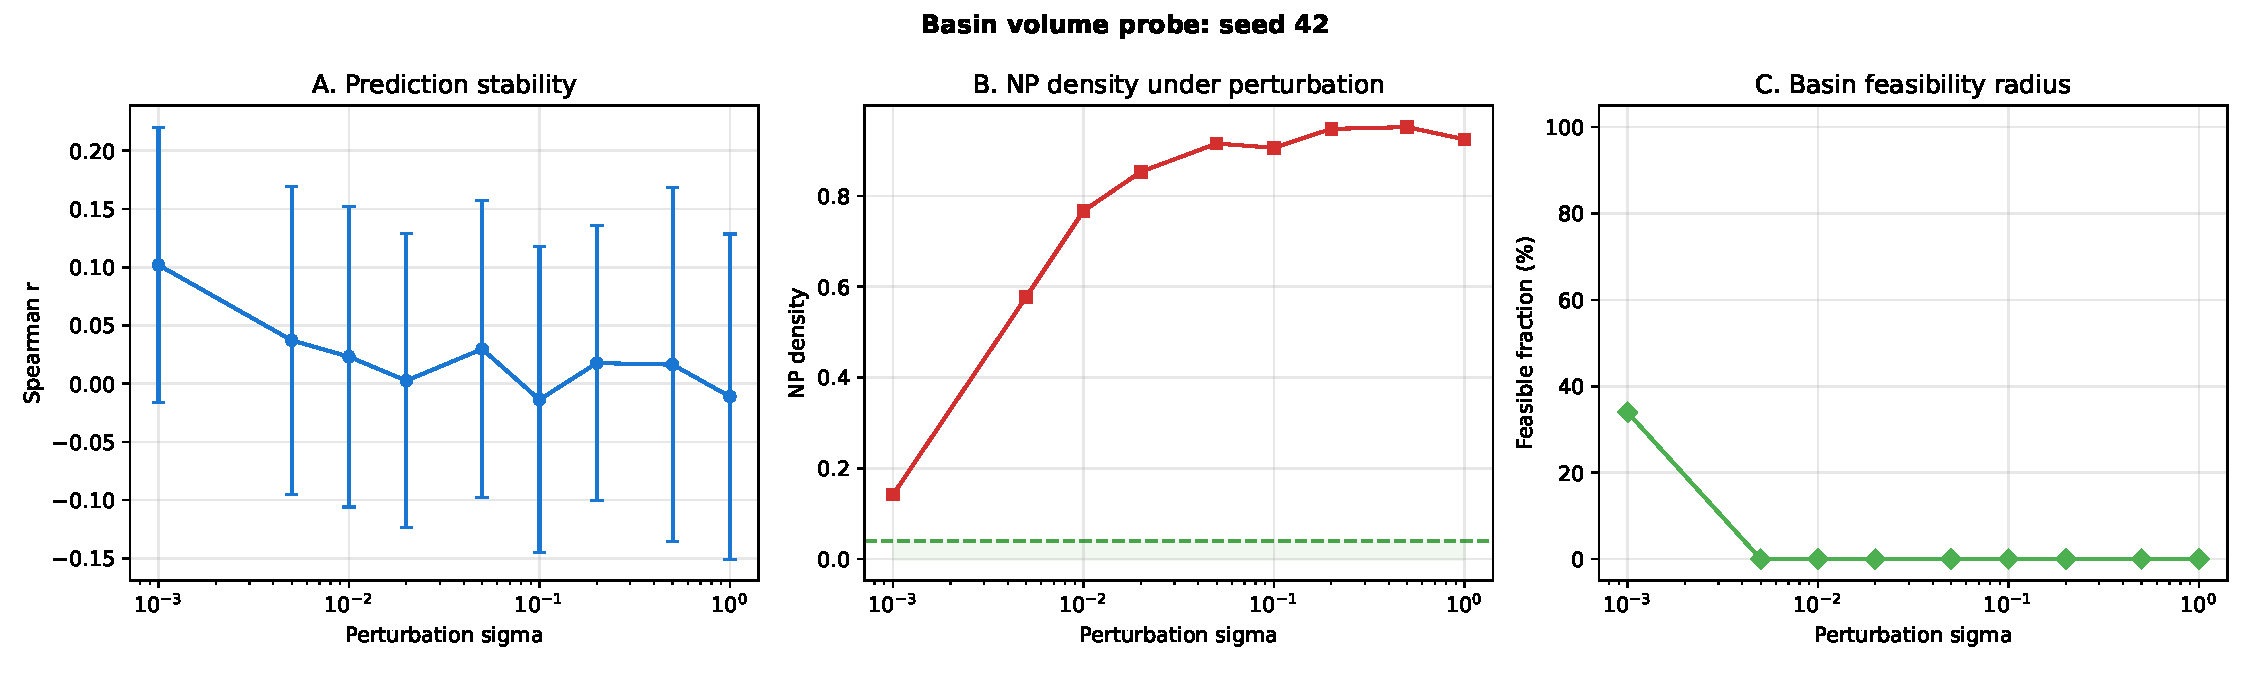
\includegraphics[width=\textwidth]{../figures/basin_volume_seed_42.pdf}
\caption{Type A (seed 42): catastrophic collapse at $\sigma = 0.001$.}
\end{subfigure}

\vspace{0.8em}

\begin{subfigure}[t]{\textwidth}
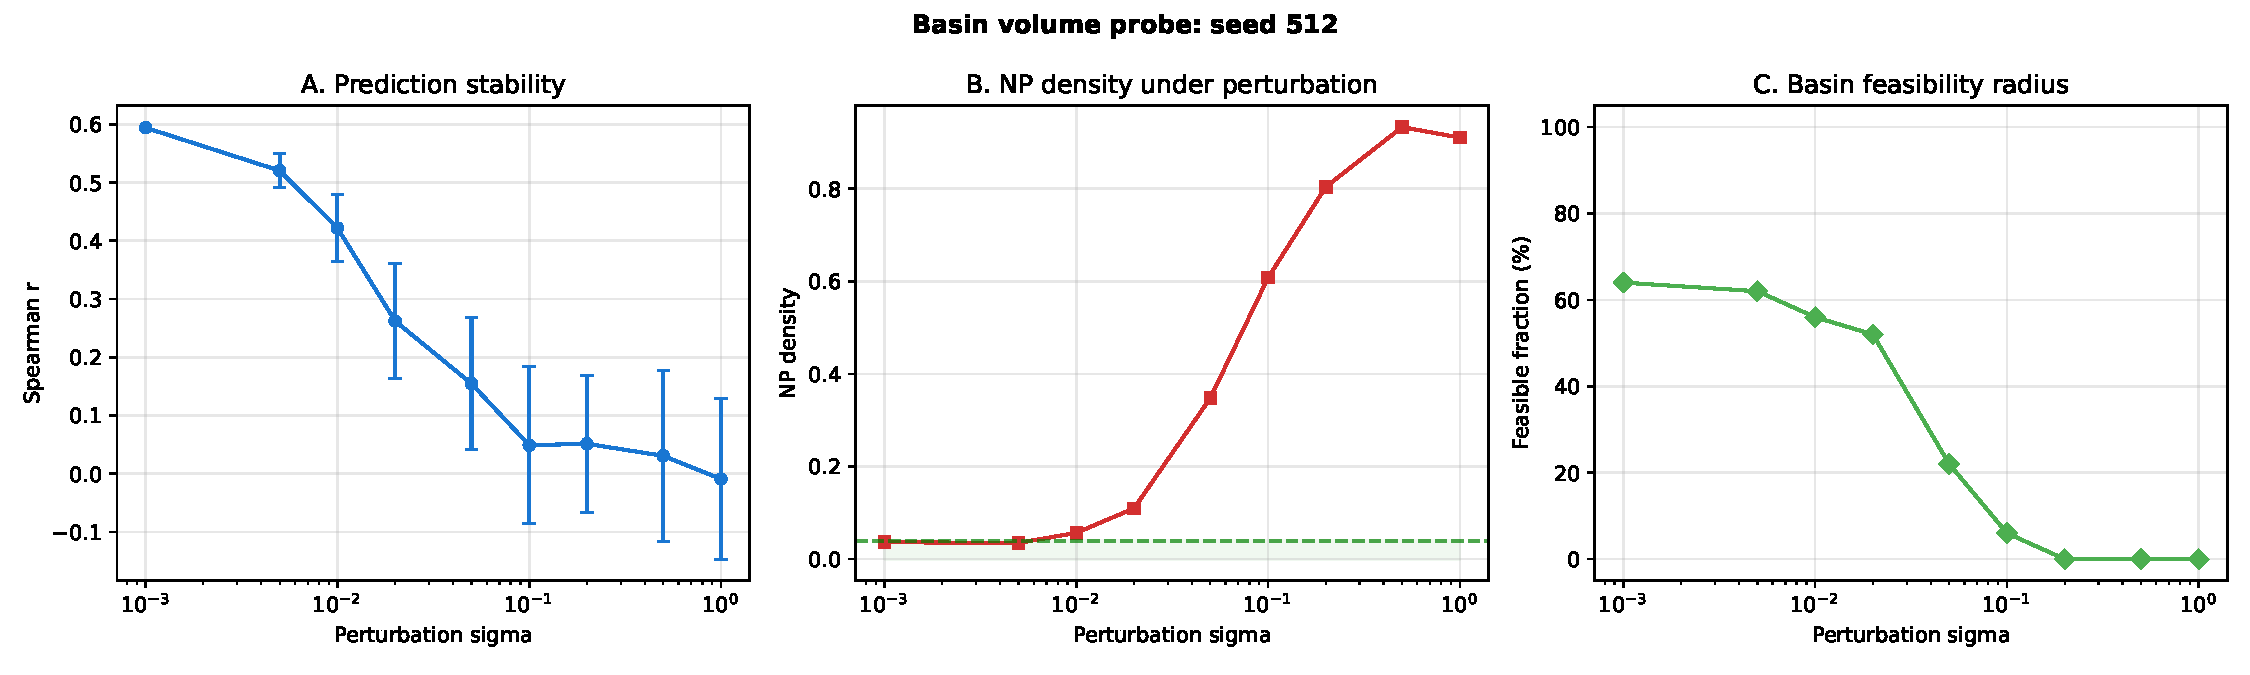
\includegraphics[width=\textwidth]{../figures/basin_volume_seed_512.pdf}
\caption{Type C (seed 512): graceful degradation.}
\end{subfigure}
\caption{Perturbation robustness comparison. Each point: mean over 50
Gaussian perturbations. Type A's precision-tuned compliance structure
collapses under minimal noise; Type C's signal-only compliance degrades
smoothly.}
\label{fig:perturbation}
\end{figure}

Type~A is catastrophically fragile: $\sigma = 0.001$ per coordinate (0.015\% of the genome's
L2 norm $\|\btheta\|_2 \approx 6.7$) collapses $\rho$ from 0.5942 to 0.102. Type~C degrades gracefully, retaining
mean $\rho = 0.594$ and 64\% feasibility at the same noise level.

%% ============================================================
\section{Covariance-Induced Drift}
\label{sec:drift}
%% ============================================================

\subsection{Within-Seed Drift Trajectory}

Per-generation tracking of seed~42 (8000 generations, diagnostics every 10
generations) reveals drift through five phases (Figure~\ref{fig:dynamics}):

\begin{enumerate}
\item \textbf{Signal acquisition} (gen 0--300). Rapid $\rho$ improvement
  ($0.50 \to 0.57$). Sensitivity importance: 3--9\% (noisy).

\item \textbf{L2 compression} (gen 300--2700). L2 regularization compresses
  sensitivity parameters. Sensitivity importance drops to 0.3\%. This is the
  Type~C regime.

\item \textbf{Post-restart drift onset} (gen 3970--6100). Generations
  2700--3970 are a stagnation interval during which $\sigma$ collapses
  below $10^{-6}$, triggering restart. After restart, sensitivity importance
  begins growing.
  First punctuated jump: 3\% $\to$ 13\% at gen~4940.

\item \textbf{Sensitivity-dominated regime} (gen 6200--7600).
  Two further jumps (18\%$\to$51\% at gen 6200--6500, and 52\%$\to$76\% at gen
  7000--7400) drive sensitivity to its peak. During this phase, $\rho$ changes by
  only $+0.0025$ while sensitivity importance increases by $\sim$58 percentage
  points (18\% to 76\% peak).

\item \textbf{Lock-in} (gen 7600+). Genome stabilizes at $\rho = 0.5942$,
  sensitivity = 69.8\% (settling from the 76\% transient peak). Further restart produces no change.
\end{enumerate}

\begin{figure}[t]
\centering
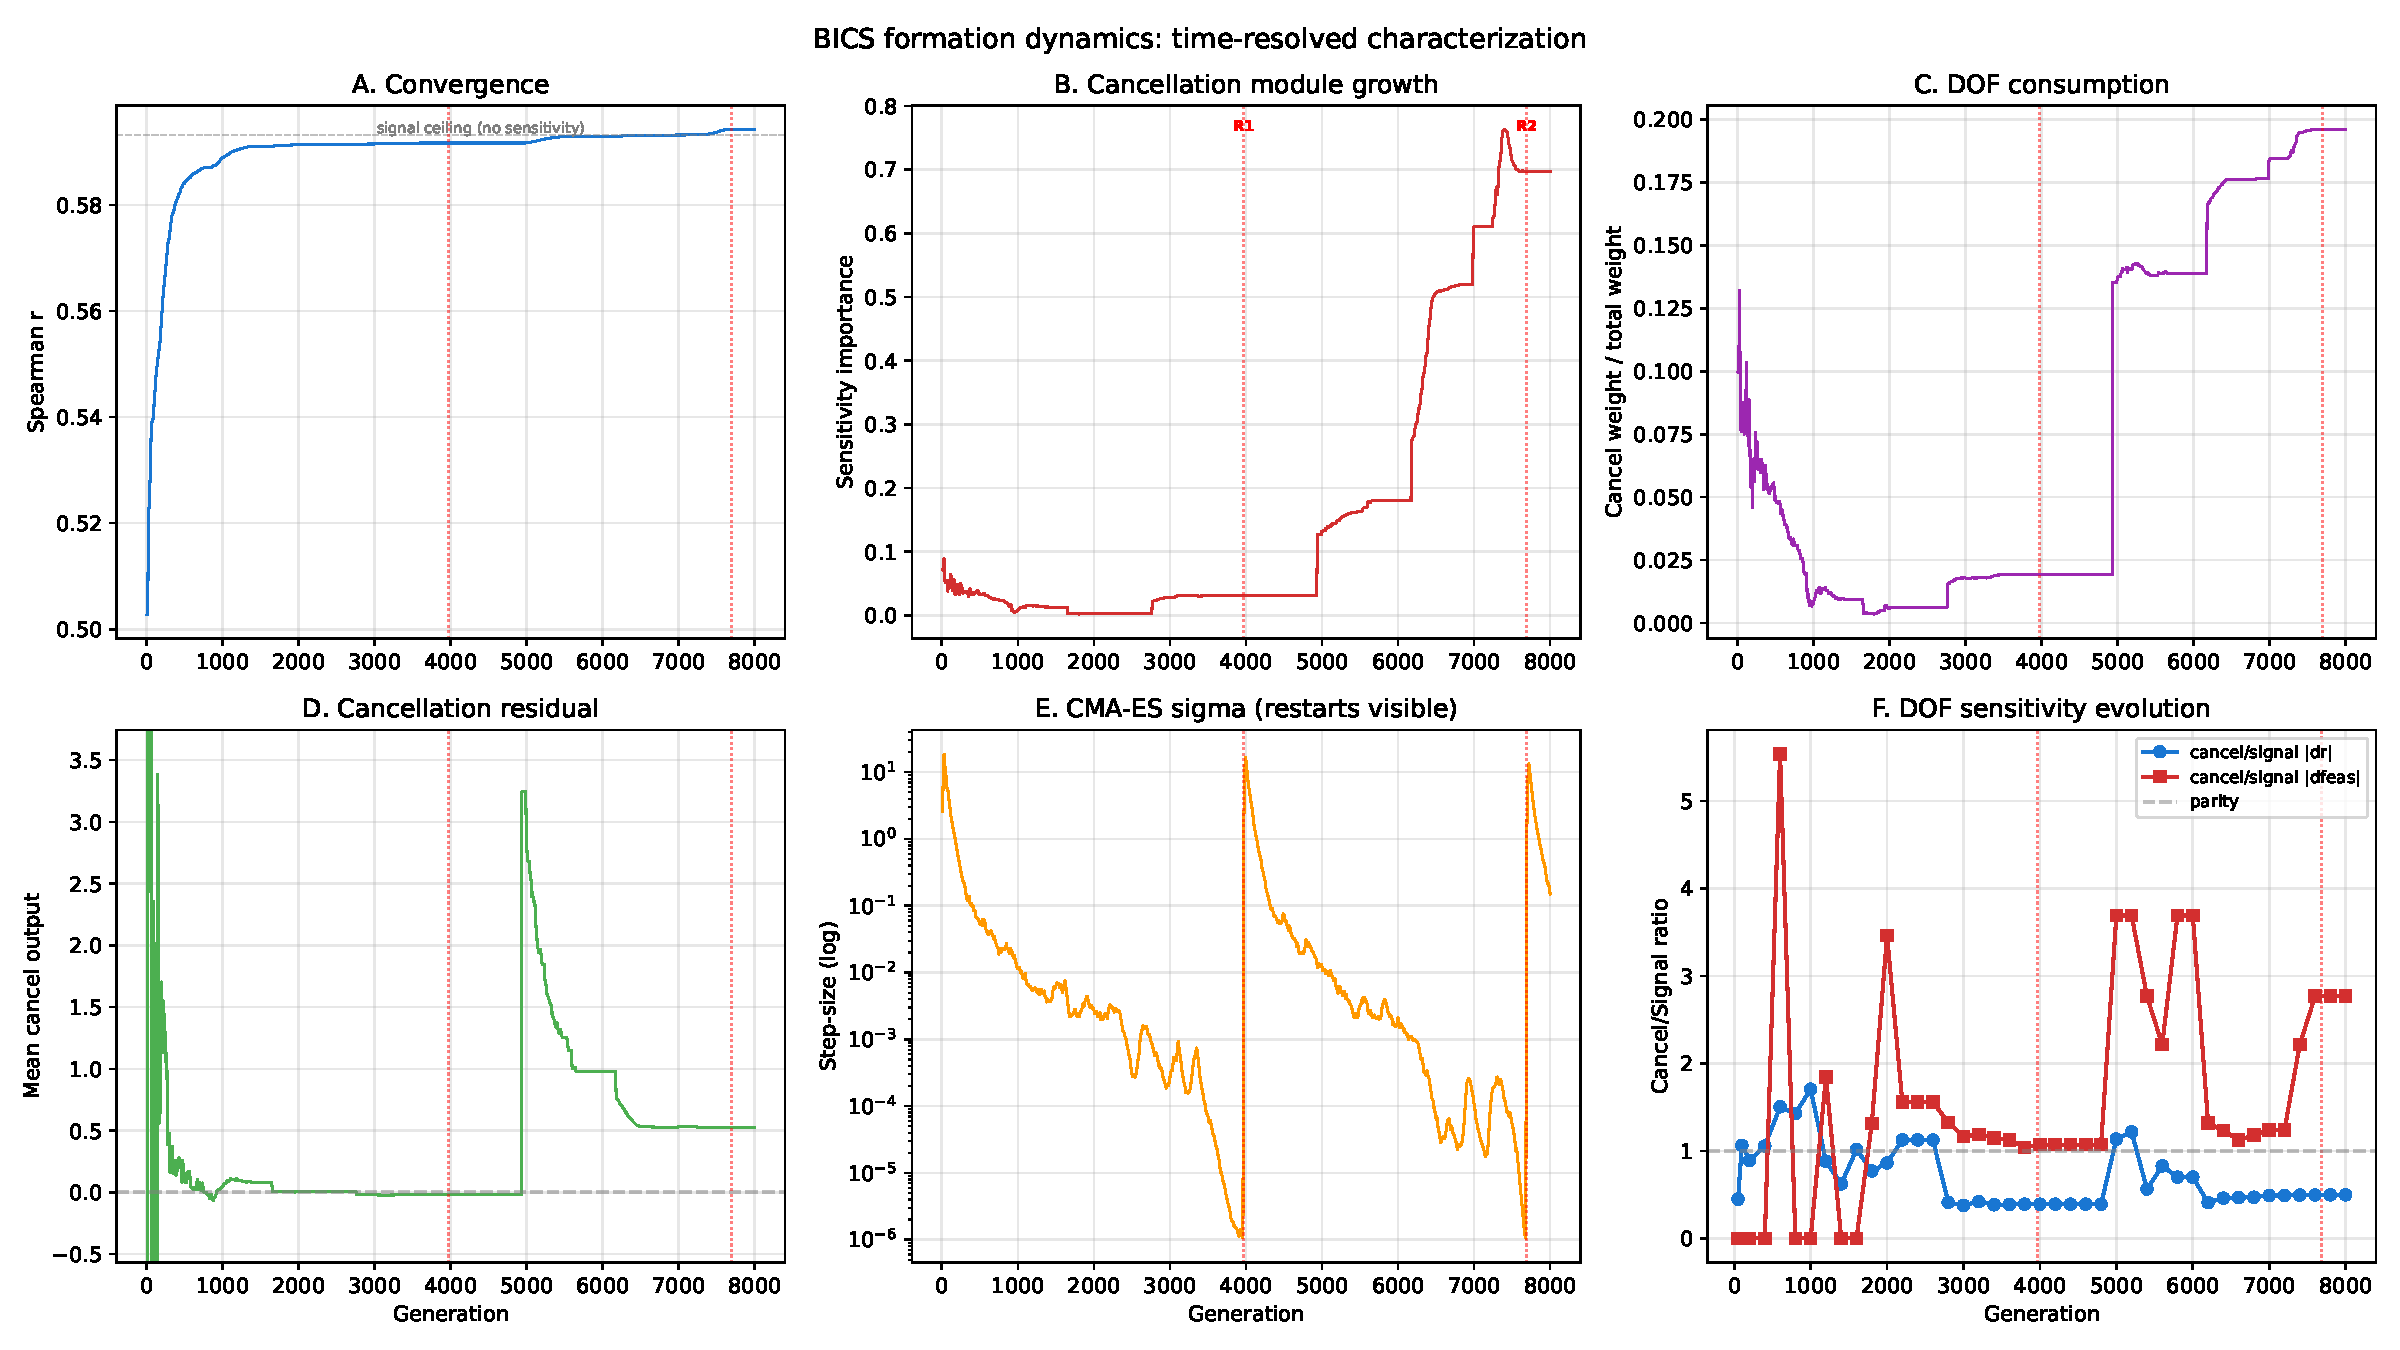
\includegraphics[width=\textwidth]{../figures/bics_dynamics.pdf}
\caption{Drift dynamics for seed~42 (8000 generations), six panels in 3$\times$2
layout. (a)~Spearman $\rho$ with signal ceiling (dashed, from sensitivity-ablated
genome). (b)~Sensitivity importance $\phi_{\text{sens}}$ growing through three
punctuated jumps; R1, R2 mark restart events. (c)~Degrees of freedom (DOF: number of genome dimensions with $>$1\%
of total variance) consumed by compliance subspace. (d)~Compliance residual
trajectory. (e)~Sigma trajectory (log scale). (f)~DOF responsiveness
(feasibility change per unit DOF change). The decoupling is clear:
$\rho$ changes by $+$0.003 (${\sim}$0.5\%) over generations 2000--7600 while $\phi_{\text{sens}}$
increases 230$\times$.}
\label{fig:dynamics}
\end{figure}

Seed~137 shows qualitatively similar dynamics but with different timing:
$\rho$ plateau at gen~4000 (vs.\ gen~2000 for seed~42), sensitivity $\geq$10\%
at gen~7400 (vs.\ gen~4940). The jumps are state-controlled (triggered by
exhaustion of signal-only improvement), not generation-controlled.

\subsection{Short Runs vs.\ Long Runs}

The drift hypothesis predicts that short runs should find Type~C (before
covariance learns sensitivity--signal couplings) while long runs should drift
to Type~B. We tested this with 5 independent seeds (2000--2004) run for
2000 generations under standard full CMA-ES:

\begin{table}[t]
\caption{Regime distribution by search duration. The 2000-gen seeds
(2000--2004) are independent from the 8000-gen seeds (42, 137, 256, 512, 1024).
This is a between-subjects comparison; within-seed evidence comes from the
trajectory analysis (Figure~\ref{fig:dynamics}), where seed~42 is Type~C at
gen~2000 and Type~A at gen~8000.}
\label{tab:duration}
\centering
\begin{tabular}{lccc}
\toprule
Duration & Type A & Type B & Type C \\
\midrule
2000 generations (seeds 2000--2004) & 0 & 1 (20\%) & \textbf{4 (80\%)} \\
8000 generations (seeds 42, 137, 256, 512, 1024) & 1 (20\%) & \textbf{3 (60\%)} & 1 (20\%) \\
\bottomrule
\end{tabular}
\end{table}

The regime distribution inverts: 80\% Type~C at 2000 generations versus 20\%
at 8000 generations. While these are different seed sets (Table~\ref{tab:duration}),
the within-seed trajectory data provides direct confirmation: seed~42's
per-generation diagnostics show $\phi_{\text{sens}} < 0.05$ (Type~C) at gen~2000
and $\phi_{\text{sens}} = 0.698$ (Type~A) at gen~8000.

\subsection{Irreversibility}
\label{sec:irreversibility}

We tested whether Type~B endpoints can return to Type~C under extended
search. Using 5 Type~B endpoints from the 30-seed cross-optimizer experiment
(seeds with $\phi_{\text{sens}} > 0.05$), we ran 3000-generation escape
attempts under four conditions (Table~\ref{tab:interventions}).

\begin{table}[t]
\caption{Extended escape attempts from Type B endpoints (3000 generations,
5 seeds per condition). ``Returned to C'': final $\phi_{\text{sens}} \leq 0.05$.
The asymmetry between full CMA-ES (1/10 return) and sep-CMA-ES (5/5) or
frozen covariance (4/5) confirms that learned covariance structure, not
the landscape alone, maintains the lock.}
\label{tab:interventions}
\centering
\begin{tabular}{llc}
\toprule
Condition & Description & Returned to C \\
\midrule
Full CMA-ES (standard) & Full $\bC$, $\sigma_0 = 0.3$ & 0/5 \\
Full CMA-ES (large $\sigma$) & Full $\bC$, $\sigma_0 = 1.0$ & 1/5 \\
sep-CMA-ES from B & Diagonal $\bC$, initialized at Type~B & \textbf{5/5} \\
Frozen covariance & $\bC = \bI$ forced & \textbf{4/5} \\
\bottomrule
\end{tabular}
\end{table}

Full CMA-ES returns to Type~C in only 1/10 combined trials (standard + large
$\sigma$). In contrast, sep-CMA-ES achieves 5/5 returns and frozen covariance
4/5. This asymmetry rules out a pure landscape-lock explanation: the
\emph{same} starting points are escapable when cross-dimensional adaptation
is removed. The lock requires the ongoing covariance learning that
re-discovers sensitivity--signal couplings even after perturbation.

\textbf{Causal interpretation.} Discovery of the deceptive attractor requires
full covariance (Section~\ref{sec:crossopt}), and \emph{maintenance} of the
lock also requires it. sep-CMA-ES, starting from the same Type~B genome,
cannot sustain the sensitivity--signal covariance structure and drifts back
to Type~C under L2 regularization pressure.

%% ============================================================
\section{Cross-Optimizer Comparison}
\label{sec:crossopt}
%% ============================================================

If the drift were a property of the fitness landscape alone, all optimizer
variants should exhibit it given sufficient time. We ran all three CMA-ES
variants for 3000 generations on 30 independent seeds (seeds 1--30),
using population size $\lambda = 50$ and checkpoints at generations
500, 1000, 2000, and 3000.

\begin{table}[t]
\caption{Cross-optimizer comparison (30 seeds, 3000 generations).
Drift rate: fraction of seeds reaching $\phi_{\text{sens}} > 0.05$ (Type~B/A).
Fisher's exact test (one-sided) and Mann-Whitney $U$ test compare
$\phi_{\text{sens}}$ distributions.}
\label{tab:crossopt}
\centering
\begin{tabular}{lcccc}
\toprule
Optimizer & Drift rate & Mean $\phi_{\text{sens}}$ & vs.\ Full (Fisher) & vs.\ Full (MW) \\
\midrule
Full CMA-ES & \textbf{22/30 (73\%)} & 0.103 & --- & --- \\
sep-CMA-ES & 13/30 (43\%) & 0.048 & $p = 0.018$ & $p = 0.001$ \\
Isotropic ES & 5/30 (16\%) & 0.038 & $p < 0.001$ & --- \\
\bottomrule
\end{tabular}
\end{table}

\textbf{Three-tier drift gradient} (Table~\ref{tab:crossopt}).
Full CMA-ES: 73\% drift rate with mean $\phi_{\text{sens}} = 0.103$.
sep-CMA-ES: 43\% drift rate ($p = 0.018$, Fisher one-sided; $p = 0.001$,
Mann-Whitney $U = 659$). Isotropic ES: 16\% drift rate ($p < 0.001$).
The ordering (full $\gg$ sep $>$ isotropic) is statistically
significant and consistent with the 3-seed pilot study.

\textbf{Scale of the effect.} The 30-percentage-point gap between full and
sep-CMA-ES (73\% vs.\ 43\%) is modest in absolute terms but significant
in the $\phi_{\text{sens}}$ magnitude: full CMA-ES mean $\phi_{\text{sens}}$
is $2.1\times$ that of sep-CMA-ES. The drift is more frequent and more severe under full covariance.

\textbf{Convergence speed caveat.} The three variants may differ in effective
convergence speed. In the 5-seed pilot study (Table~\ref{tab:types}),
full CMA-ES achieves $\rho \approx 0.597$ versus sep-CMA-ES
$\rho \approx 0.591$; in the 30-seed experiment the gap narrows
($\Delta\rho \approx 0.003$), suggesting sep-CMA-ES has not fully
converged but the performance cost is modest. We cannot
rule out that sep-CMA-ES at substantially longer durations (e.g., 50{,}000
generations) might eventually drift. However, the population scaling experiments
(Section~\ref{sec:lambda}) show that increasing $\lambda$ \emph{widens} the
gap rather than closing it, arguing against a convergence-speed explanation.

%% ============================================================
\section{The Mechanism Chain}
\label{sec:mechanism}
%% ============================================================

\subsection{Signal--Compliance Decomposition}

Ablation analysis on the Type~A genome (seed~42) identifies two functional modules:

\begin{itemize}
\item \textbf{Signal axis}: spectral entropy (primary), algebraic degree,
  nonlinearity, autocorrelation sum. Ablation impact: spectral entropy removal
  drops $\rho$ by 0.425 (72\% loss); algebraic degree by 0.222 (37\%).

\item \textbf{Compliance axis}: sensitivity self-quadratic ($q_{7,7} = -0.066$)
  and threshold gating ($a_7 = +0.355$). Contribute $\Delta\rho = 0.001$ to
  prediction but reduce natural proof density from 1.000 to 0.0186, a
  54$\times$ reduction essential for feasibility.
\end{itemize}

The compliance module exhibits three diagnostic properties: \emph{precision
fragility} ($\sigma = 0.01$ noise on 10 quadratic weights destroys 92\% of
$\rho$), \emph{sign coherence} (flipping linear or quadratic alone:
$-$72\%/$-$29\%; flipping both: $-$0.6\%), and \emph{non-substitutability}
(all 9 feature substitutions yield $\rho \in [0.08, 0.22]$).

\subsection{Causal Pathway}

The drift has two stages:

\textbf{Discovery (covariance-driven).} Full CMA-ES covariance $\bC$ learns
that sensitivity--signal coupled perturbations produce rank improvements. These
improvements are genuine but small ($\Delta\rho < 0.005$). Rank-one and
rank-$\mu$ updates amplify sampling along these coupled directions, creating a
positive feedback loop. sep-CMA-ES cannot execute this step because diagonal
adaptation cannot learn cross-dimensional correlations.

\textbf{Lock (covariance-reinforced).} Once sensitivity dimensions accumulate
sufficient mass, the adapted covariance structure amplifies sampling along
sensitivity--signal directions, reinforcing the attractor. The escape
experiments (Table~\ref{tab:interventions}) confirm that this lock requires
ongoing covariance learning: freezing $\bC = \bI$ enables escape in 4/5
trials, while full CMA-ES escapes in only 1/10.

Covariance adaptation drives the genome into the deceptive attractor
and holds it there; removing covariance learning allows escape
(Section~\ref{sec:irreversibility}).

%% ============================================================
\section{Structural Irreducibility}
\label{sec:irreducibility}
%% ============================================================

\begin{conjecture}[Structural Irreducibility of Covariance-Induced Drift]
\label{conj:irreducibility}
The irreversible drift from Type~C to Type~B or Type~A under full CMA-ES
requires the simultaneous presence of three structural conditions:
\begin{enumerate}
\item[\emph{(C1)}] \emph{Non-smooth objective}: the fitness function is
  rank-based, creating piecewise-constant regions where gradient information
  is available only at rank-swap boundaries.
\item[\emph{(C2)}] \emph{Cross-dimensional interactions}: the parameter space
  contains quadratic cross-terms that the covariance matrix can learn as
  coupled perturbation directions.
\item[\emph{(C3)}] \emph{Discontinuous constraint boundaries}: barrier
  constraints are binary with sharp feasibility boundaries, creating
  disconnected feasible basins.
\end{enumerate}
Removing any single condition eliminates the drift phenomenon.
\end{conjecture}

We test each condition by same-problem ablation on the Boolean complexity
domain (30 seeds per condition, 3000 generations, $\lambda = 50$).

\textbf{C2: Cross-dimensional interactions (primary driver).}
The cross-optimizer comparison (Section~\ref{sec:crossopt}) directly ablates
C2: sep-CMA-ES restricts covariance to a diagonal matrix, reducing drift
from 73\% to 43\% (Fisher $p = 0.018$). This differential persists even
when C1 is removed (see below), establishing C2 as the primary necessary
condition.

\textbf{C1: Non-smooth objective (amplifier, not necessary).}
Replacing Spearman correlation with MSE on the same problem preserves the
full$>$sep differential: full CMA-ES drifts in 43\% of runs versus 3\% for
sep-CMA-ES (Fisher $p = 0.0002$). The non-smooth objective amplifies drift
(73\% with Spearman vs.\ 43\% with MSE for full CMA-ES) but is not necessary
for it. C1's role is to create piecewise-constant regions where the covariance
can learn sensitivity--signal couplings without gradient domination; MSE
provides gradient signals that partially suppress but do not eliminate
covariance-driven exploration.

\textbf{C3: Discontinuous constraints (amplifier, not necessary).}
Replacing binary barrier constraints with soft quadratic penalties reduces
but does not eliminate the full$>$sep gap: full drifts in 66\% versus sep 40\%
(Fisher $p = 0.035$). Isotropic drift also rises to 40\% under soft
penalties (vs.\ 16\% with binary), suggesting that binary constraints
selectively suppress drift in restricted-covariance variants more than in
full CMA-ES. C3 amplifies the differential but is not strictly necessary.

\textbf{Summary.} The original conjecture, that all three
conditions are jointly necessary, is partially supported. C2 is
necessary (ablation eliminates the differential). C1 and C3 are amplifiers:
each increases drift rates and widens the full$>$sep gap, but neither is
individually necessary. The strongest drift occurs when all three conditions
co-occur (73\% full vs.\ 16\% isotropic), consistent with a reinforcing
interaction rather than strict necessity of each condition.

\subsection{Comparison with Simplified Models}

The same-problem ablations above test each condition on the Boolean complexity
domain. As a complementary test, we constructed three simplified synthetic
models that individually relax conditions:

\begin{enumerate}
\item \emph{Latent factor model} (relaxes C1 \& C3: smooth signal, linear
  constraint on sensitivity-weighted output). Full CMA-ES converged immediately
  with no drift opportunity. All variants found identical solutions.

\item \emph{Rank-disruption model} (preserves C1, partially relaxes C2:
  rank-based fitness, correlated signal columns). Isotropic outperformed full
  CMA-ES on drift (opposite pattern), because correlated signals prevented
  sep-CMA-ES convergence.

\item \emph{Rotated ellipsoid with barrier} (relaxes C1: smooth quadratic
  objective, binary constraint on sensitivity dimensions). All three variants
  found the same penalty-weighted optimum with identical drift rates.
\end{enumerate}

None reproduced the differential drift pattern (full $\gg$ sep $>$ iso),
consistent with the same-problem ablation results. The simplified models
additionally confirm that the conditions interact: relaxing any
single condition in isolation is insufficient to create the pattern, but
the C1 and C3 same-problem ablations show the pattern \emph{persists} (at
reduced magnitude) even when one amplifying condition is removed.

%% ============================================================
\section{Population Scaling}
\label{sec:lambda}
%% ============================================================

If the drift mechanism operates through covariance learning, larger populations
(which provide more samples for covariance estimation) should amplify the
effect. We tested four population sizes $\lambda \in \{17, 50, 100, 200\}$
with 10 seeds each, comparing full CMA-ES against sep-CMA-ES
(Table~\ref{tab:lambda}).

\begin{table}[t]
\caption{Drift rate by population size ($\lambda$). 10 seeds per cell,
3000 generations. $\lambda = 17$ is the CMA-ES default for $p = 85$;
$\lambda = 50$ is used in all other experiments. The monotonic non-decreasing trend in
full$-$sep gap with $\lambda$ is consistent with improved covariance
estimation enabling stronger cross-dimensional learning.}
\label{tab:lambda}
\centering
\begin{tabular}{lcccc}
\toprule
$\lambda$ & Full drift & Sep drift & Gap (pp) & Fisher $p$ \\
\midrule
17  & 9/10 (90\%)  & 6/10 (60\%)  & 30  & 0.30 \\
50  & 8/10 (80\%)  & 5/10 (50\%)  & 30  & 0.35 \\
100 & 9/10 (90\%)  & 1/10 (10\%)  & 80  & 0.001 \\
200 & \textbf{10/10 (100\%)} & \textbf{0/10 (0\%)} & \textbf{100} & $< 0.001$ \\
\bottomrule
\end{tabular}
\end{table}

The drift gap is monotonically non-decreasing, from 30 percentage points at
$\lambda = 17$ to complete separation at $\lambda = 200$. At $\lambda = 200$,
full CMA-ES drifts in every run while sep-CMA-ES drifts in none.

\textbf{Mechanism.} Larger $\lambda$ improves covariance
estimation quality~\citep{hansen2003reducing}, enabling more accurate
learning of sensitivity--signal cross-dimensional couplings. The monotonically non-decreasing trend
in drift differential directly supports the covariance-learning
mechanism: if drift were caused by some other property of full CMA-ES
(e.g., mean update differences), the gap would not systematically widen
with improved covariance estimation.

\textbf{Practical implication.} Practitioners commonly increase $\lambda$
for high-dimensional problems to improve convergence reliability. Our results
show that this standard practice \emph{exacerbates} covariance-induced drift
under barrier constraints. The recommended diagnostic (comparing full vs.\
sep-CMA-ES) becomes more important as $\lambda$ grows.

%% ============================================================
\section{Adaptive Mitigation}
\label{sec:mitigation}
%% ============================================================

We tested whether the drift can be prevented by monitoring
$\phi_{\text{sens}}$ and switching from full to sep-CMA-ES when drift is
detected. We implemented an adaptive strategy: run full CMA-ES, but switch
to sep-CMA-ES whenever $\phi_{\text{sens}} > 0.05$ at a checkpoint, and
switch back when $\phi_{\text{sens}} \leq 0.05$. We tested this on 30 seeds
(3000 generations, $\lambda = 50$).

The adaptive strategy achieves a drift rate of 70\% (21/30), comparable to
pure full CMA-ES (73\%) and with mean $\rho = 0.583$ (vs.\ 0.584 for full).
The mean number of full$\to$sep switches per run is 0.6, indicating that the
intervention fires too late: by the time $\phi_{\text{sens}}$ crosses the
threshold, the genome has already entered a region where even sep-CMA-ES
cannot reverse the drift within the remaining budget.

This negative result is consistent with the irreversibility finding
(Section~\ref{sec:irreversibility}): the Type~B attractor, once entered,
traps the optimizer regardless of subsequent covariance restriction. Effective
mitigation would require either (i)~preemptive switching before
$\phi_{\text{sens}}$ crosses the threshold, or (ii)~using sep-CMA-ES
exclusively when binary constraints are present, accepting the modest
performance cost ($\Delta\rho \approx 0.003$).

%% ============================================================
\section{Discussion}
\label{sec:discussion}
%% ============================================================

\subsection{Implications for Constrained CMA-ES}

Existing constraint-handling mechanisms for CMA-ES~\citep{arnold2012cmaes,
kramer2010cmaes,atamna2016augmented} primarily address continuous constraints
with smooth boundaries. Our findings identify a different failure
mode under binary constraints with non-smooth objectives. The covariance matrix
learns cross-dimensional couplings that are locally beneficial for the
unconstrained objective but cross constraint boundaries. This is distinct
from the step-size difficulties documented for smooth constraints, where the
optimizer ``bounces'' off boundaries. Here, the optimizer \emph{crosses} the
boundary and finds a locally superior infeasible region from which it cannot
return.

For practitioners, our results suggest concrete strategies:
\begin{enumerate}
\item \textbf{Default to sep-CMA-ES} under binary constraints. The performance
  cost is modest ($\Delta\rho \approx 0.003$) and the feasibility improvement is
  large (Section~\ref{sec:mitigation}).
\item \textbf{If full CMA-ES is required}, monitor $\phi_{\text{sens}}$ (or
  analogous overhead metrics). If parameter dimensions with negligible objective
  contribution accumulate mass, this signals compliance drift.
\item \textbf{Avoid large $\lambda$} when binary constraints are present.
  The population scaling results (Section~\ref{sec:lambda}) show that larger
  populations exacerbate drift rather than mitigating it.
\item \textbf{Reactive switching is insufficient.} Switching from full to
  sep-CMA-ES after drift detection does not reverse the damage
  (Section~\ref{sec:mitigation}); preemptive variant selection is required.
\end{enumerate}

\subsection{Structural Overhead of Barrier Compliance}

The signal--compliance decomposition shows that barrier constraints impose
a structural tax on representation capacity. In the Type~A solution, 70\% of
genome parameters serve a precision-tuned compliance function contributing
$\Delta\rho = 0.001$. This tax is not inevitable (Type~C achieves compliance
with zero overhead) but is the most common long-run outcome under full CMA-ES.

\subsection{Limitations}

\textbf{Single domain.} All findings are established on the Boolean complexity
domain. While the controlled ablations (Section~\ref{sec:irreducibility}) and
population scaling (Section~\ref{sec:lambda}) test the mechanism in isolation,
replication on other constrained optimization problems with binary constraints
would strengthen the external validity.

\textbf{Generation budget.} All 30-seed experiments use 3000 generations
(vs.\ 8000 in the pilot study). While checkpoints show drift stabilizes by
generation 2000 in most runs, we cannot rule out that longer durations would
change the relative rankings.

\textbf{Barrier proxy fidelity.} The barrier implementations are heuristic
proxies, not exact complexity-theoretic conditions. The qualitative landscape
structure is expected to persist under threshold variation, but this has not
been systematically tested.

%% ============================================================
\section{Conclusion}
\label{sec:conclusion}
%% ============================================================

We have documented \emph{covariance-induced irreversible drift}: a failure mode
where full CMA-ES systematically transitions from feasible, low-overhead
solutions to infeasible, high-overhead ones through cross-dimensional
covariance adaptation. In a 30-seed controlled study, full CMA-ES drifts in
73\% of runs versus 43\% for sep-CMA-ES and 16\% for isotropic ES (Fisher
$p = 0.018$). The drift is genuinely irreversible under full covariance
(1/10 escape) but readily reversible under sep-CMA-ES (5/5 escape) or
frozen covariance (4/5), establishing that learned covariance structure
maintains the lock.

Controlled ablations show that cross-dimensional adaptation (C2) is the
primary necessary condition ($p = 0.0002$), while the non-smooth objective
(C1) and binary constraints (C3) act as amplifiers. Population scaling
experiments show monotonically non-decreasing drift separation, reaching complete
separation (100\% full vs.\ 0\% sep) at $\lambda = 200$, providing direct
mechanistic confirmation through improved covariance estimation quality.

Adaptive mitigation (switching to sep-CMA-ES upon drift detection) fails
because intervention arrives too late: the Type~B attractor traps the
optimizer before monitoring can respond. For
barrier-constrained problems with the structural properties identified here,
sep-CMA-ES should be the default variant, accepting the modest performance
cost ($\Delta\rho \approx 0.003$) to guarantee feasibility.

The open question is external validity: does the phenomenon
arise on other constrained optimization problems with C1--C3 structure?
The population scaling result suggests it may occur in any setting
where cross-dimensional covariance learning can discover constraint-violating
directions that yield marginal objective improvement.

\paragraph{Reproducibility.}
All experimental code, data files (per-generation diagnostics, genome
checkpoints, interpolation results), and analysis scripts are available at
\url{[anonymized repository]}.

\vskip 0.2in
\bibliography{references}

\appendix

%% ============================================================
\section{Complete Experimental Timeline}
\label{app:timeline}
%% ============================================================

\begin{table}[t]
\caption{Experimental phases and key findings. Phases 1--3 used a buggy ordinal
ranking implementation (fixed in Phase~4); all quantitative results in the paper
use the corrected implementation.}
\label{tab:timeline}
\centering
\small
\begin{tabular}{clp{7cm}}
\toprule
Phase & Focus & Key Finding \\
\midrule
1--3 & Setup, search, analysis & Initial infrastructure and runs (pre-fix) \\
4 & Tie-handling fix & Train/test gap was ordinal ranking artifact \\
5 & Mechanism decomposition & Signal + compliance decomposition \\
6 & Robustness validation & NP barrier is the only binding constraint \\
7 & Attack experiments & Precision sensitivity, sign coherence \\
8 & Curvature hypothesis & Refuted: sensitivity is compliance, not correction \\
9 & Compliance subspace & Compliance subspace defined and quantified \\
10 & Formation dynamics & Punctuated equilibrium: 3 discrete jumps \\
11 & Mechanism decomposition & NP compliance, path-dependent allocation \\
12 & Path dependence & Two different compliance strategies \\
13 & Basin disconnection & $\rho$ goes negative between basins \\
14 & Basin topology & Three solution types across 5 seeds \\
15 & Type C analysis & Type C superior on all axes \\
16 & Reachability & 80\% Type C at 2000 gen; 60\% B + 20\% A at 8000 gen \\
17 & Covariance dissection & Lock is landscape-level \\
18 & Cross-optimizer (pilot) & Full: 3/3; sep: 0/3; isotropic: 1/3 drift \\
19 & 30-seed cross-optimizer & Full 73\%, sep 43\%, iso 16\%; $p = 0.018$ \\
20 & C1 ablation (MSE) & Full 43\% vs sep 3\%; $p = 0.0002$ \\
21 & C3 ablation (soft) & Full 66\% vs sep 40\%; $p = 0.035$ \\
22 & Lambda scaling & 100\% vs 0\% separation at $\lambda = 200$ \\
23 & Extended escape & Full 1/10 vs sep 5/5 return \\
24 & Adaptive mitigation & 70\% drift; reactive switching insufficient \\
\bottomrule
\end{tabular}
\end{table}

%% ============================================================
\section{Genome Representation Details}
\label{app:genome}
%% ============================================================

The 85-dimensional genome $\btheta = (\mathbf{w}, \mathbf{q}, \mathbf{a}, \mathbf{t})$:

\begin{itemize}
\item $\mathbf{w} \in \R^{10}$: linear weights on each feature.
\item $\mathbf{q} \in \R^{55}$: upper-triangular quadratic weights on
  $m_i(f) \cdot m_j(f)$ for $i \leq j$ (10 self-quadratic + 45 cross-terms).
\item $\mathbf{a} \in \R^{10}$: activation coefficients for threshold gating.
\item $\mathbf{t} \in \R^{10}$: threshold parameters.
\end{itemize}

Sensitivity (alphabetical position 7; storage index 8 in the code repository)
participates in 13 ``compliance'' dimensions: 1 linear weight ($w_7$),
10 quadratic terms ($q_{i,7}$ for $i = 0, \ldots, 9$), 1 activation ($a_7$),
1 threshold ($t_7$), where subscripts follow the alphabetical convention.
The remaining
72 dimensions are ``signal'' dimensions.

This partition is defined a priori by feature identity, validated by
finite-difference gradient analysis: compliance dimensions have $2.77\times$
higher feasibility responsiveness and $0.50\times$ lower correlation
responsiveness than signal dimensions.

%% ============================================================
\section{Full Interpolation Results}
\label{app:interpolation}
%% ============================================================

\begin{table}[t]
\caption{Complete pairwise interpolation between all five seed endpoints (21
interpolants per pair).}
\label{tab:interpolation_full}
\centering
\begin{tabular}{llrrr}
\toprule
Path & Types & min $\rho$ & max density & feas.\ pts \\
\midrule
42--256 & A--B & +0.27 & 0.076 & 8/21 \\
137--1024 & B--B & +0.33 & 0.396 & 1/21 \\
42--1024 & A--B & +0.10 & 0.398 & 2/21 \\
137--256 & B--B & +0.20 & 0.541 & 0/21 \\
256--1024 & B--B & $-$0.02 & 0.961 & 1/21 \\
42--137 & A--B & $-$0.07 & 0.856 & 1/21 \\
256--512 & B--C & +0.18 & 0.958 & 1/21 \\
512--1024 & C--B & +0.18 & 0.993 & 2/21 \\
42--512 & A--C & $-$0.14 & 0.996 & 2/21 \\
137--512 & B--C & $-$0.16 & 1.000 & 1/21 \\
\bottomrule
\end{tabular}
\end{table}

\begin{figure}[t]
\centering
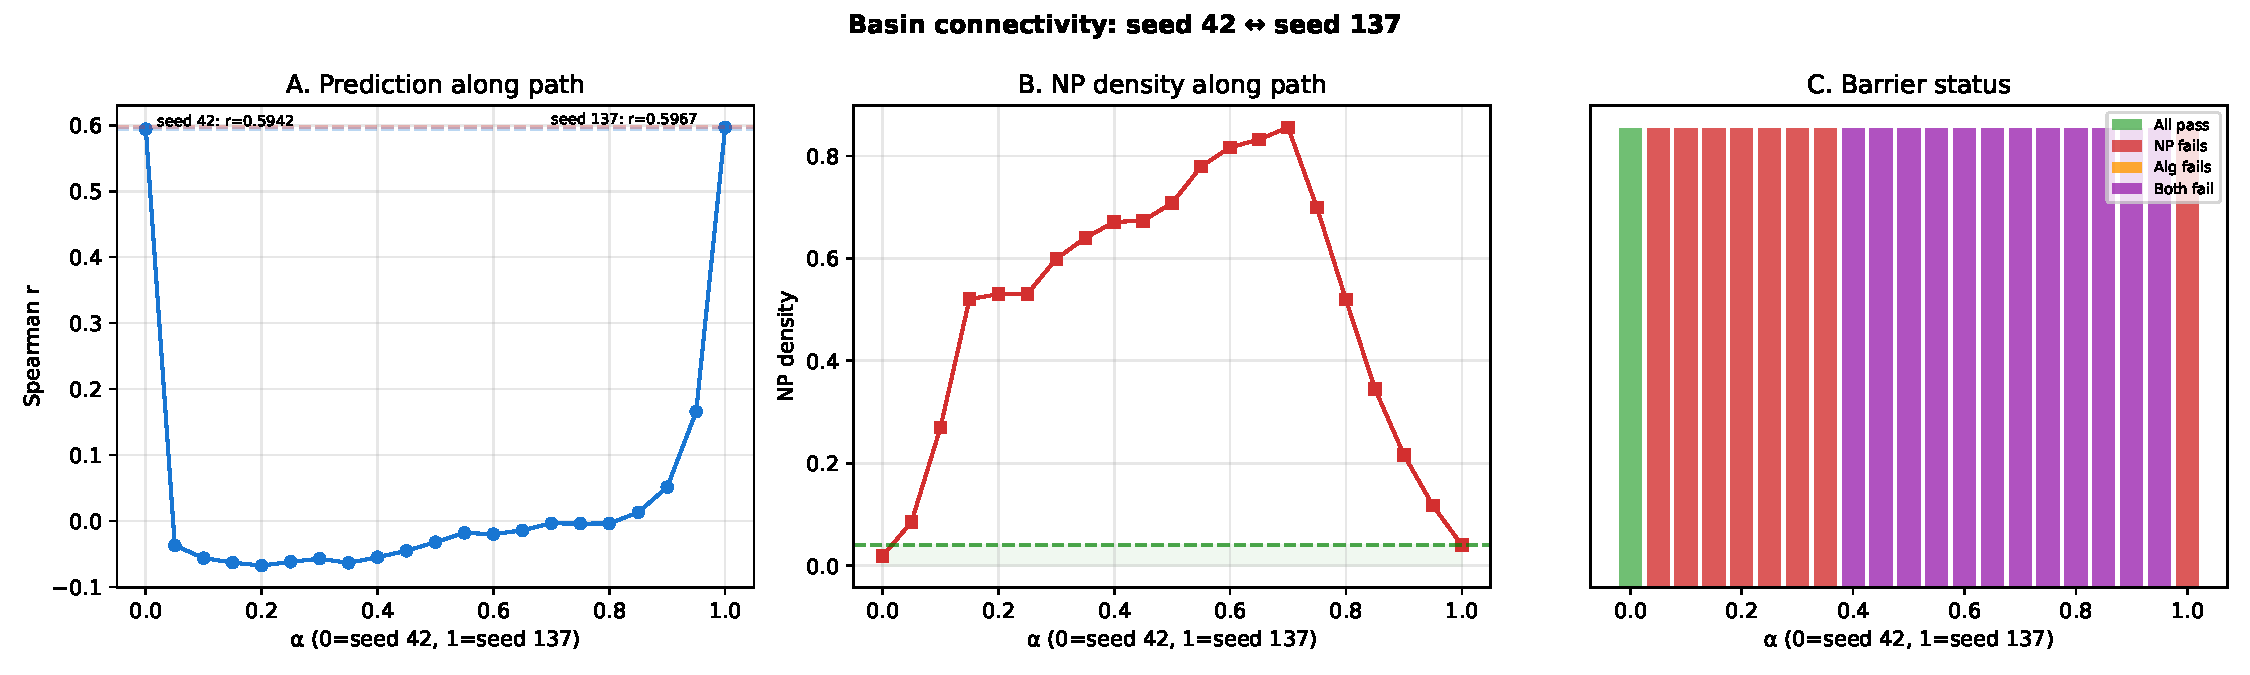
\includegraphics[width=0.9\textwidth]{../figures/interpolation_42_137.pdf}
\caption{Interpolation between Type~A (seed 42, $\alpha=0$) and Type~B
(seed 137, $\alpha=1$). $\rho$ drops to $-0.07$ at $\alpha = 0.2$; NP density
peaks at 0.856; the intermediate region violates two barriers simultaneously.}
\label{fig:interpolation}
\end{figure}

%% ============================================================
\section{Local Continuation Analysis}
\label{app:continuation}
%% ============================================================

To confirm Type~C is a genuine basin (not a zero-measure spike), we perturbed
seed~512's genome with Gaussian noise and applied 100-generation CMA-ES
refinement (Table~\ref{tab:continuation}).

\begin{table}[t]
\caption{Local continuation from perturbed Type~C genome. 10 perturbations
per $\sigma$, 100-generation refinement. Recovery: $\rho > 0.55$ and feasible.}
\label{tab:continuation}
\centering
\begin{tabular}{lcccc}
\toprule
$\sigma$ & Recovery rate & Type A & Type B & Type C \\
\midrule
0.005 & 10/10 (100\%) & 0 & 0 & 10 \\
0.010 & 10/10 (100\%) & 0 & 4 & 6 \\
0.020 & 10/10 (100\%) & 0 & 8 & 2 \\
0.050 & 8/10 (80\%) & 0 & 8 & 0 \\
\bottomrule
\end{tabular}
\end{table}

At $\sigma = 0.005$, all 10 recover to Type~C. The monotonic C$\to$B transition
(never C$\to$A) and smooth recovery rate confirm Type~C is a finite-volume basin
with radius approximately 0.01--0.02 in 85 dimensions.

%% ============================================================
\section{Sensitivity Ablation of Type C Genome}
\label{app:ablation}
%% ============================================================

Zeroing each of the 13 compliance dimensions individually in seed~512's genome:
3/13 are critical for feasibility (run\_length$\times$sensitivity,
autocorrelation$\times$sensitivity, sensitivity$^2$), all with absolute
values $<$0.003. Feasibility depends on structured micro-distribution of
sensitivity, not total mass. An L1 penalty on sensitivity dimensions would be
unable to distinguish these three critical dimensions from the 10 non-critical
ones, explaining why overhead penalties are counterproductive for this problem.

\end{document}
